%! TEX program = xelatex
%---------------------------------------------------------------------------%
%-                                                                         -%
%-                           LaTeX Template                                -%
%-                                                                         -%
%---------------------------------------------------------------------------%
%- Copyright (C) Huangrui Mo <huangrui.mo@gmail.com> 
%- This is free software: you can redistribute it and/or modify it
%- under the terms of the GNU General Public License as published by
%- the Free Software Foundation, either version 3 of the License, or
%- (at your option) any later version.
%---------------------------------------------------------------------------%
%->> Document class declaration
%---------------------------------------------------------------------------%
\documentclass[doublesided, fontset=mac]{Style/ucasthesis}%
%- Multiple optional arguments:
%- [<singlesided|doublesided|printcopy>]% set one or two sided eprint or print
%- [fontset=<adobe|...>]% specify font set to replace automatic detection
%- [plain]% thesis writing of international students
%- [draftversion]% show draft version information
%- [standard options for ctex book class: draft|paper size|font size|...]%
%---------------------------------------------------------------------------%
%->> Document settings
%---------------------------------------------------------------------------%
\usepackage[numbers,myhdr,list]{Style/artratex}% document settings
%- usage: \usepackage[option1,option2,...,optionN]{artratex}
%- Multiple optional arguments:
%- [bibtex|biber]% set bibliography processor and package
%- [<numbers|super|authoryear|alpha>]% set citation and reference style
%- <numbers>: textual: Jones [1]; parenthetical: [1]
%- <super>: textual: Jones superscript [1]; parenthetical: superscript [1]
%- <authoryear>: textual: Jones (1995); parenthetical: (Jones, 1995)
%- <alpha>: textual: not available; parenthetical: [Jon95]
%- [geometry]% reconfigure page layout via geometry package
%- [lscape]% provide landscape layout environment
%- [myhdr]% enable header and footer via fancyhdr package
%- [color]% provide color support via xcolor package
%- [background]% enable page background
%- [tikz]% provide complex diagrams via tikz package
%- [table]% provide complex tables via ctable package
%- [list]% provide enhanced list environments for algorithm and coding
%- [math]% enable some extra math packages
\usepackage{Style/artracom}% user defined commands
%---------------------------------------------------------------------------%
%->> Document inclusion
%---------------------------------------------------------------------------%
%\includeonly{Tex/Chap_1,...,Tex/Chap_N}% selected files compilation
%---------------------------------------------------------------------------%
%->> Document content
%---------------------------------------------------------------------------%
\newcommand\dprime{\prime\prime}
\newcommand\tprime{\prime\prime\prime}
\begin{document}
%-
%-> Frontmatter: title page, abstract, content list, symbol list, preface
%-
\frontmatter% initialize the environment
%---------------------------------------------------------------------------%
%->> 封面信息及生成
%---------------------------------------------------------------------------%
%-
%-> 中文封面信息
%-
\confidential{}% 密级:只有涉密论文才填写
\schoollogo{scale=0.095}{ucas_logo}% 校徽
\title{拐点暴胀模型}% 论文中文题目
\author{徐武涛}% 论文作者
\advisor{郭宗宽~研究员~中国科学院理论物理研究所}% 指导教师:姓名 专业技术职务 工作单位
\advisors{}% 指导老师附加信息 或 第二指导老师信息
\degree{博士}% 学位:学士、硕士、博士
\degreetype{理学}% 学位类别:理学、工学、工程、医学等
\major{理论物理}% 二级学科专业名称
\institute{中国科学院理论物理研究所}% 院系名称
\date{2019~年~12~月}% 毕业日期:夏季为6月、冬季为12月
%-
%-> 英文封面信息
%-
\TITLE{Inflection Point Inflation}% 论文英文题目
\AUTHOR{Xu Wutao}% 论文作者
\ADVISOR{Supervisor: Professor Guo Zongkuan}% 指导教师
\DEGREE{Doctor}% 学位:Bachelor, Master, Doctor。封面格式将根据英文学位名称自动切换,请确保拼写准确无误
\DEGREETYPE{Philosophy}% 学位类别:Philosophy, Natural Science, Engineering, Economics, Agriculture 等
\MAJOR{Theoretical Physics}% 二级学科专业名称
\INSTITUTE{Institute of Theoretical Physics, Chinese Academy of Sciences}% 院系名称
\DATE{December, 2019}% 毕业日期:夏季为June、冬季为December
%-
%-> 生成封面
%-
\maketitle% 生成中文封面
\MAKETITLE% 生成英文封面
%-
%-> 作者声明
%-
\makedeclaration% 生成声明页
%-
%-> 中文摘要
%-
\intobmk\chapter*{摘\quad 要}% 显示在书签但不显示在目录
\setcounter{page}{1}% 开始页码
\pagenumbering{Roman}% 页码符号


本文首先介绍了现代宇宙学的基本理论。包含标准宇宙学模型中的背景演化,以及遭遇到的
一些疑难问题。然后是以此为背景发展出的暴胀宇宙学,介绍了基本的理论模型。接着着重
介绍了工作相关的规范扰动理论,包括三种扰动类型、各自满足的规范不变方程组。并以
标量扰动为例在某些情况下推导了扰动方程,并讨论了解的性质。以标量扰动和张量扰动为例
介绍了相关的功率谱的计算。


\keywords{宇宙微波背景辐射,原初黑洞,二级引力波,慢滚参数}% 中文关键词
%-
%-> 英文摘要
%-
\intobmk\chapter*{Abstract}% 显示在书签但不显示在目录

write lately.

\KEYWORDS{cosmic microwave background, primodial black hole, second order
gravitional wave, slow-roll parameters}% 英文关键词
%---------------------------------------------------------------------------%
% title page, abstract, dedication
{% content list region
\linespread{1.2}% local line space
\intobmk*{\cleardoublepage}{\contentsname}% add link to bookmark
\tableofcontents% content catalog
\intobmk*{\cleardoublepage}{\listfigurename}% add link to bookmark
\listoffigures% figure catalog
\intobmk*{\cleardoublepage}{\listtablename}% add link to bookmark
\listoftables% table catalog
}
\intobmk\chapter*{符号列表}% 显示在书签但不显示在目录

\section*{字符}
\nomenclatureitem[\textbf{Unit}]{\textbf{Symbol}}{\textbf{Description}}
\nomenclatureitem[$\Unit{m^{2} \cdot s^{-2} \cdot K^{-1}}$]{$R$}{the gas constant}
\nomenclatureitem[$\Unit{m^{2} \cdot s^{-2} \cdot K^{-1}}$]{$C_v$}{specific heat capacity at constant volume}
\nomenclatureitem[$\Unit{m^{2} \cdot s^{-2} \cdot K^{-1}}$]{$C_p$}{specific heat capacity at constant pressure}
\nomenclatureitem[$\Unit{m^{2} \cdot s^{-2}}$]{$E$}{specific total energy}
\nomenclatureitem[$\Unit{m^{2} \cdot s^{-2}}$]{$e$}{specific internal energy}
\nomenclatureitem[$\Unit{m^{2} \cdot s^{-2}}$]{$h_T$}{specific total enthalpy}
\nomenclatureitem[$\Unit{m^{2} \cdot s^{-2}}$]{$h$}{specific enthalpy}
\nomenclatureitem[$\Unit{kg \cdot m \cdot s^{-3} \cdot K^{-1}}$]{$k$}{thermal conductivity}
\nomenclatureitem[$\Unit{kg \cdot m^{-1} \cdot s^{-2}}$]{$S_{ij}$}{deviatoric stress tensor}
\nomenclatureitem[$\Unit{kg \cdot m^{-1} \cdot s^{-2}}$]{$\tau_{ij}$}{viscous stress tensor}
\nomenclatureitem[$\Unit{1}$]{$\delta_{ij}$}{Kronecker tensor}
\nomenclatureitem[$\Unit{1}$]{$I_{ij}$}{identity tensor}

\section*{算子}
\nomenclatureitem{\textbf{Symbol}}{\textbf{Description}}
\nomenclatureitem{$\Delta$}{difference}
\nomenclatureitem{$\nabla$}{gradient operator}
\nomenclatureitem{$\delta^{\pm}$}{upwind-biased interpolation scheme}

\section*{缩写}
\nomenclatureitem{CFD}{Computational Fluid Dynamics}
\nomenclatureitem{CFL}{Courant-Friedrichs-Lewy}
\nomenclatureitem{EOS}{Equation of State}
\nomenclatureitem{JWL}{Jones-Wilkins-Lee}
\nomenclatureitem{WENO}{Weighted Essentially Non-oscillatory}
\nomenclatureitem{ZND}{Zel'dovich-von Neumann-Doering}

% list of symbols, preface content
%-
%-> Mainmatter
%-
\mainmatter% initialize the environment
%---------------------------------------------------------------------------%
%->> Main content
%---------------------------------------------------------------------------%
% \chapter{引言}\label{chap:introduction}

\section{研究背景}

考虑到许多同学可能缺乏\LaTeX{}使用经验,ucasthesis将\LaTeX{}的复杂性高度封装,开放出简单的接口,以便轻易使用。同时,对用\LaTeX{}撰写论文的一些主要难题,如制图、制表、文献索引等,进行了详细说明,并提供了相应的代码样本,理解了上述问题后,对于初学者而言,使用此模板撰写学位论文将不存在实质性的困难。所以,如果你是初学者,请不要直接放弃,因为同样为初学者的我,十分明白让\LaTeX{}简单易用的重要性,而这正是ucasthesis所追求和体现的。

此中国科学院大学学位论文模板ucasthesis基于中科院数学与系统科学研究院吴凌云研究员的CASthesis模板发展而来。当前ucasthesis模板满足最新的中国科学院大学学位论文撰写要求和封面设定。兼顾操作系统:Windows,Linux,MacOS 和\LaTeX{}编译引擎:pdflatex,xelatex,lualatex。支持中文书签、中文渲染、中文粗体显示、拷贝PDF中的文本到其他文本编辑器等特性。此外,对模板的文档结构进行了精心设计,撰写了编译脚本提高模板的易用性和使用效率。

ucasthesis的目标在于简化学位论文的撰写,利用\LaTeX{}格式与内容分离的特征,模板将格式设计好后,作者可只需关注论文内容。 同时,ucasthesis有着整洁一致的代码结构和扼要的注解,对文档的仔细阅读可为初学者提供一个学习\LaTeX{}的窗口。此外,模板的架构十分注重通用性,事实上,ucasthesis不仅是国科大学位论文模板,同时,通过少量修改即可成为使用\LaTeX{}撰写中英文文章或书籍的通用模板,并为使用者的个性化设定提供了接口。

\section{系统要求}\label{sec:system}

\href{https://github.com/mohuangrui/ucasthesis}{\texttt{ucasthesis}} 宏包可以在目前主流的 \href{https://en.wikibooks.org/wiki/LaTeX/Introduction}{\LaTeX{}} 编译系统中使用,如\TeX{}Live和MiK\TeX{}。因C\TeX{}套装已停止维护,\textbf{不再建议使用} (请勿混淆C\TeX{}套装与ctex宏包。C\TeX{}套装是集成了许多\LaTeX{}组件的\LaTeX{}编译系统。 \href{https://ctan.org/pkg/ctex?lang=en}{ctex} 宏包如同ucasthesis,是\LaTeX{}命令集,其维护状态活跃,并被主流的\LaTeX{}编译系统默认集成,是几乎所有\LaTeX{}中文文档的核心架构)。推荐的 \href{https://en.wikibooks.org/wiki/LaTeX/Installation}{\LaTeX{}编译系统} 和 \href{https://en.wikibooks.org/wiki/LaTeX/Installation}{\LaTeX{}文本编辑器} 为
\begin{center}
    %\footnotesize% fontsize
    %\setlength{\tabcolsep}{4pt}% column separation
    %\renewcommand{\arraystretch}{1.5}% row space 
    \begin{tabular}{lcc}
        \hline
        %\multicolumn{num_of_cols_to_merge}{alignment}{contents} \\
        %\cline{i-j}% partial hline from column i to column j
        操作系统 & \LaTeX{}编译系统 & \LaTeX{}文本编辑器\\
        \hline
        Linux & \href{https://www.tug.org/texlive/acquire-netinstall.html}{\TeX{}Live Full} & \href{http://www.xm1math.net/texmaker/}{Texmaker} 或 Vim (已集成于 Linux 系统)\\
        MacOS & \href{https://www.tug.org/mactex/}{Mac\TeX{} Full} & \href{http://www.xm1math.net/texmaker/}{Texmaker} 或 Texshop (已集成于 Mac\TeX{} Full)\\
        Windows & \href{https://www.tug.org/texlive/acquire-netinstall.html}{\TeX{}Live Full} 或 \href{https://miktex.org/download}{MiK\TeX{}} & \href{http://www.xm1math.net/texmaker/}{Texmaker}\\
        \hline
    \end{tabular}
\end{center}

\LaTeX{}编译系统,如\TeX{}Live(Mac\TeX{}为针对MacOS的\TeX{}Live),用于提供编译环境,\LaTeX{}文本编辑器 (如Texmaker) 用于编辑\TeX{}源文件。请从各软件官网下载安装程序,勿使用不明程序源。\textbf{\LaTeX{}编译系统和\LaTeX{}编辑器分别安装成功后,即完成了\LaTeX{}的系统配置},无需其他手动干预和配置。若系统原带有旧版的\LaTeX{}编译系统并想安装新版,请\textbf{先卸载干净旧版再安装新版}。

\section{问题反馈}

关于\LaTeX{}的知识性问题,请查阅 \href{https://github.com/mohuangrui/ucasthesis/wiki}{ucasthesis知识小站} 和 \href{https://en.wikibooks.org/wiki/LaTeX}{\LaTeX{} Wikibook}。

关于模板编译和样式设计的问题,请\textbf{先仔细阅读此说明文档,特别是“常见问题”(章节~\ref{sec:qa})}。若问题仍无法得到解决,请\textbf{先将问题理解清楚并描述清楚,再将问题反馈}至 \href{https://github.com/mohuangrui/ucasthesis/issues}{Github/ucasthesis/issues}。

欢迎大家有效地反馈模板不足之处,一起不断改进模板。希望大家向同事积极推广\LaTeX{},一起更高效地做科研。

\section{模板下载}

\begin{center}
    \href{https://github.com/mohuangrui/ucasthesis}{Github/ucasthesis}: \url{https://github.com/mohuangrui/ucasthesis}
\end{center}

% \chapter{\LaTeX{}使用说明}\label{chap:guide}

为方便使用及更好地展示\LaTeX{}排版的优秀特性,ucasthesis的框架和文件体系进行了细致地处理,尽可能地对各个功能和板块进行了模块化和封装,对于初学者来说,众多的文件目录也许一开始让人觉得有些无所适从,但阅读完下面的使用说明后,会发现原来使用思路是简单而清晰的,而且,当对\LaTeX{}有一定的认识和了解后,会发现其相对Word类排版系统极具吸引力的优秀特性。所以,如果是初学者,请不要退缩,请稍加尝试和坚持,以领略到\LaTeX{}的非凡魅力,并可以通过阅读相关资料如\LaTeX{} Wikibook \citep{wikibook2014latex} 来完善自己的使用知识。

\section{先试试效果}

\begin{enumerate}
    \item 安装软件:根据所用操作系统和章节~\ref{sec:system}中的信息安装\LaTeX{}编译环境。
    \item 获取模板:下载 \href{https://github.com/mohuangrui/ucasthesis}{ucasthesis} 模板并解压。ucasthesis模板不仅提供了相应的类文件,同时也提供了包括参考文献等在内的完成学位论文的一切要素,所以,下载时,推荐下载整个ucasthesis文件夹,而不是单独的文档类。
    \item 编译模板:
        \begin{enumerate}
            \item Windows:双击运行artratex.bat脚本。
            \item Linux或MacOS: {\scriptsize \verb|terminal| -> \verb|chmod +x ./artratex.sh| -> \verb|./artratex.sh xa|}
            \item 任意系统:都可使用\LaTeX{}编辑器打开Thesis.tex文件并选择xelatex编译引擎进行编译。
        \end{enumerate}
    \item 错误处理:若编译中遇到了问题,请先查看“常见问题”(章节~\ref{sec:qa})。
\end{enumerate}

编译完成即可获得本PDF说明文档。而这也完成了学习使用ucasthesis撰写论文的一半进程。什么?这就学成一半了,这么简单???,是的,就这么简单!

\section{文档目录简介}

\subsection{Thesis.tex}

Thesis.tex为主文档,其设计和规划了论文的整体框架,通过对其的阅读可以了解整个论文框架的搭建。

\subsection{编译脚本}

\begin{itemize}
    \item Windows:双击Dos脚本artratex.bat可得全编译后的PDF文档,其存在是为了帮助不了解\LaTeX{}编译过程的初学者跨过编译这第一道坎,请勿通过邮件传播和接收此脚本,以防范Dos脚本的潜在风险。
    \item Linux或MacOS:在terminal中运行
        \begin{itemize}
            \item \verb|./artratex.sh xa|:获得全编译后的PDF文档
            \item \verb|./artratex.sh x|:快速编译模式
        \end{itemize}
    \item 全编译指运行 \verb|xelatex+bibtex+xelatex+xelatex| 以正确生成所有的引用链接,如目录,参考文献及引用等。在写作过程中若无添加新的引用,则可用快速编译,即只运行一遍\LaTeX{}编译引擎以减少编译时间。
\end{itemize}

\subsection{Tmp文件夹}

运行编译脚本后,编译所生成的文档皆存于Tmp文件夹内,包括编译得到的PDF文档,其存在是为了保持工作空间的整洁,因为好的心情是很重要的。

\subsection{Style文件夹}

包含ucasthesis文档类的定义文件和配置文件,通过对它们的修改可以实现特定的模版设定。若需更新模板,一般只需用新的样式文件替换旧的即可。

\begin{enumerate}
    \item ucasthesis.cls:文档类定义文件,论文的最核心的格式即通过它来定义的。
    \item ucasthesis.cfg:文档类配置文件,设定如目录显示为“目~录”而非“目录”。
    \item artratex.sty: 常用宏包及文档设定,如参考文献样式、文献引用样式、页眉页脚设定等。这些功能具有开关选项,常只需在Thesis.tex中的如下命令中进行启用即可,一般无需修改artratex.sty本身。
        
        \path{\usepackage[options]{artratex}} 
    \item artracom.sty:自定义命令以及添加宏包的推荐放置位置。
\end{enumerate}

\subsection{Tex文件夹}

文件夹内为论文的所有实体内容,正常情况下,这也是\textbf{使用ucasthesis撰写学文论文时,主要关注和修改的一个位置,注:所有文件都必须采用UTF-8编码,否则编译后将出现乱码文本},详细分类介绍如下:

\begin{itemize}
    \item Frontpage.tex:为论文中英文封面及中英文摘要。\textbf{论文封面会根据英文学位名称如Bachelor,Master,或是Doctor自动切换为相应的格式}。
    \item Mainmatter.tex:索引需要出现的Chapter。开始写论文时,可以只索引当前章节,以快速编译查看,当论文完成后,再对所有章节进行索引即可。
    \item Chap{\_}xxx.tex:为论文主体的各个章节,可根据需要添加和撰写。
    \item Appendix.tex:为附录内容
    \item Backmatter.tex:为发表文章信息和致谢部分等。
\end{itemize}

\subsection{Img文件夹}

用于放置论文中所需要的图类文件,支持格式有:.jpg, .png, .pdf。其中,\verb|ucas_logo.pdf|为国科大校徽。不建议为各章节图片建子目录,即使图片众多,若命名规则合理,图片查询亦是十分方便。

\subsection{Biblio文件夹}

\begin{enumerate}
    \item ref.bib:参考文献信息库。
    \item gbt7714-xxx.bst:文献样式定义文件。由 \href{https://github.com/zepinglee}{zepinglee}  开发,在最新国标的基础上对ucas进行了定制。与文献样式有关的问题,请查阅开发者所提供的文档,并建议适当追踪 \href{https://github.com/CTeX-org/gbt7714-bibtex-style/tree/ucas}{ucas 样式分支}的更新。
\end{enumerate}

\section{数学公式、图表、参考文献等功能}

\subsection{数学公式}

比如Navier-Stokes方程(方程~\eqref{eq:ns})(times text test: 1,2,3,4,5, times math test: $\mathrm{1,2,3,4,5}, 1,2,3,4,5$):
\begin{equation} \label{eq:ns}
    \adddotsbeforeeqnnum%
    \begin{cases}
        \frac{\partial \rho}{\partial t} + \nabla\cdot(\rho\Vector{V}) = 0 \ \mathrm{times\ math\ test: 1,2,3,4,5}, 1,2,3,4,5\\
        \frac{\partial (\rho\Vector{V})}{\partial t} + \nabla\cdot(\rho\Vector{V}\Vector{V}) = \nabla\cdot\Tensor{\sigma} \ \text{times text test: 1,2,3,4,5}\\
        \frac{\partial (\rho E)}{\partial t} + \nabla\cdot(\rho E\Vector{V}) = \nabla\cdot(k\nabla T) + \nabla\cdot(\Tensor{\sigma}\cdot\Vector{V})
    \end{cases}
\end{equation}
\begin{equation}
    \adddotsbeforeeqnnum%
    \frac{\partial }{\partial t}\int\limits_{\Omega} u \, \mathrm{d}\Omega + \int\limits_{S} \unitVector{n}\cdot(u\Vector{V}) \, \mathrm{d}S = \dot{\phi}
\end{equation}
\[
    \begin{split}
        \mathcal{L} \{f\}(s) &= \int _{0^{-}}^{\infty} f(t) e^{-st} \, \mathrm{d}t, \ 
        \mathscr{L} \{f\}(s) = \int _{0^{-}}^{\infty} f(t) e^{-st} \, \mathrm{d}t\\
        \mathcal{F} {\bigl (} f(x+x_{0}) {\bigr )} &= \mathcal{F} {\bigl (} f(x) {\bigr )} e^{2\pi i\xi x_{0}}, \ 
        \mathscr{F} {\bigl (} f(x+x_{0}) {\bigr )} = \mathscr{F} {\bigl (} f(x) {\bigr )} e^{2\pi i\xi x_{0}}
    \end{split}
\]

数学公式常用命令请见 \href{https://en.wikibooks.org/wiki/LaTeX/Mathematics}{WiKibook Mathematics}。artracom.sty中对一些常用数据类型如矢量矩阵等进行了封装,这样的好处是如有一天需要修改矢量的显示形式,只需单独修改artracom.sty中的矢量定义即可实现全文档的修改。

\subsection{数学环境}

\begin{axiom}
   这是一个公理。 
\end{axiom}
\begin{theorem}
   这是一个定理。 
\end{theorem}
\begin{lemma}
   这是一个引理。 
\end{lemma}
\begin{corollary}
   这是一个推论。 
\end{corollary}
\begin{assertion}
   这是一个断言。 
\end{assertion}
\begin{proposition}
   这是一个命题。 
\end{proposition}
\begin{proof}
    这是一个证明。
\end{proof}
\begin{definition}
    这是一个定义。
\end{definition}
\begin{example}
    这是一个例子。
\end{example}
\begin{remark}
    这是一个注。
\end{remark}

\subsection{表格}

请见表~\ref{tab:sample}。
\begin{table}[!htbp]
    \bicaption{这是一个样表。}{This is a sample table.}
    \label{tab:sample}
    \centering
    \footnotesize% fontsize
    \setlength{\tabcolsep}{4pt}% column separation
    \renewcommand{\arraystretch}{1.2}%row space 
    \begin{tabular}{lcccccccc}
        \hline
        行号 & \multicolumn{8}{c}{跨多列的标题}\\
        %\cline{2-9}% partial hline from column i to column j
        \hline
        Row 1 & $1$ & $2$ & $3$ & $4$ & $5$ & $6$ & $7$ & $8$\\
        Row 2 & $1$ & $2$ & $3$ & $4$ & $5$ & $6$ & $7$ & $8$\\
        Row 3 & $1$ & $2$ & $3$ & $4$ & $5$ & $6$ & $7$ & $8$\\
        Row 4 & $1$ & $2$ & $3$ & $4$ & $5$ & $6$ & $7$ & $8$\\
        \hline
    \end{tabular}
\end{table}

制图制表的更多范例,请见 \href{https://github.com/mohuangrui/ucasthesis/wiki}{ucasthesis 知识小站} 和 \href{https://en.wikibooks.org/wiki/LaTeX/Tables}{WiKibook Tables}。

\subsection{图片插入}

论文中图片的插入通常分为单图和多图,下面分别加以介绍:

单图插入:假设插入名为\verb|tc_q_criteria|(后缀可以为.jpg、.png、.pdf,下同)的图片,其效果如图\ref{fig:tc_q_criteria}。
\begin{figure}[!htbp]
    \centering
    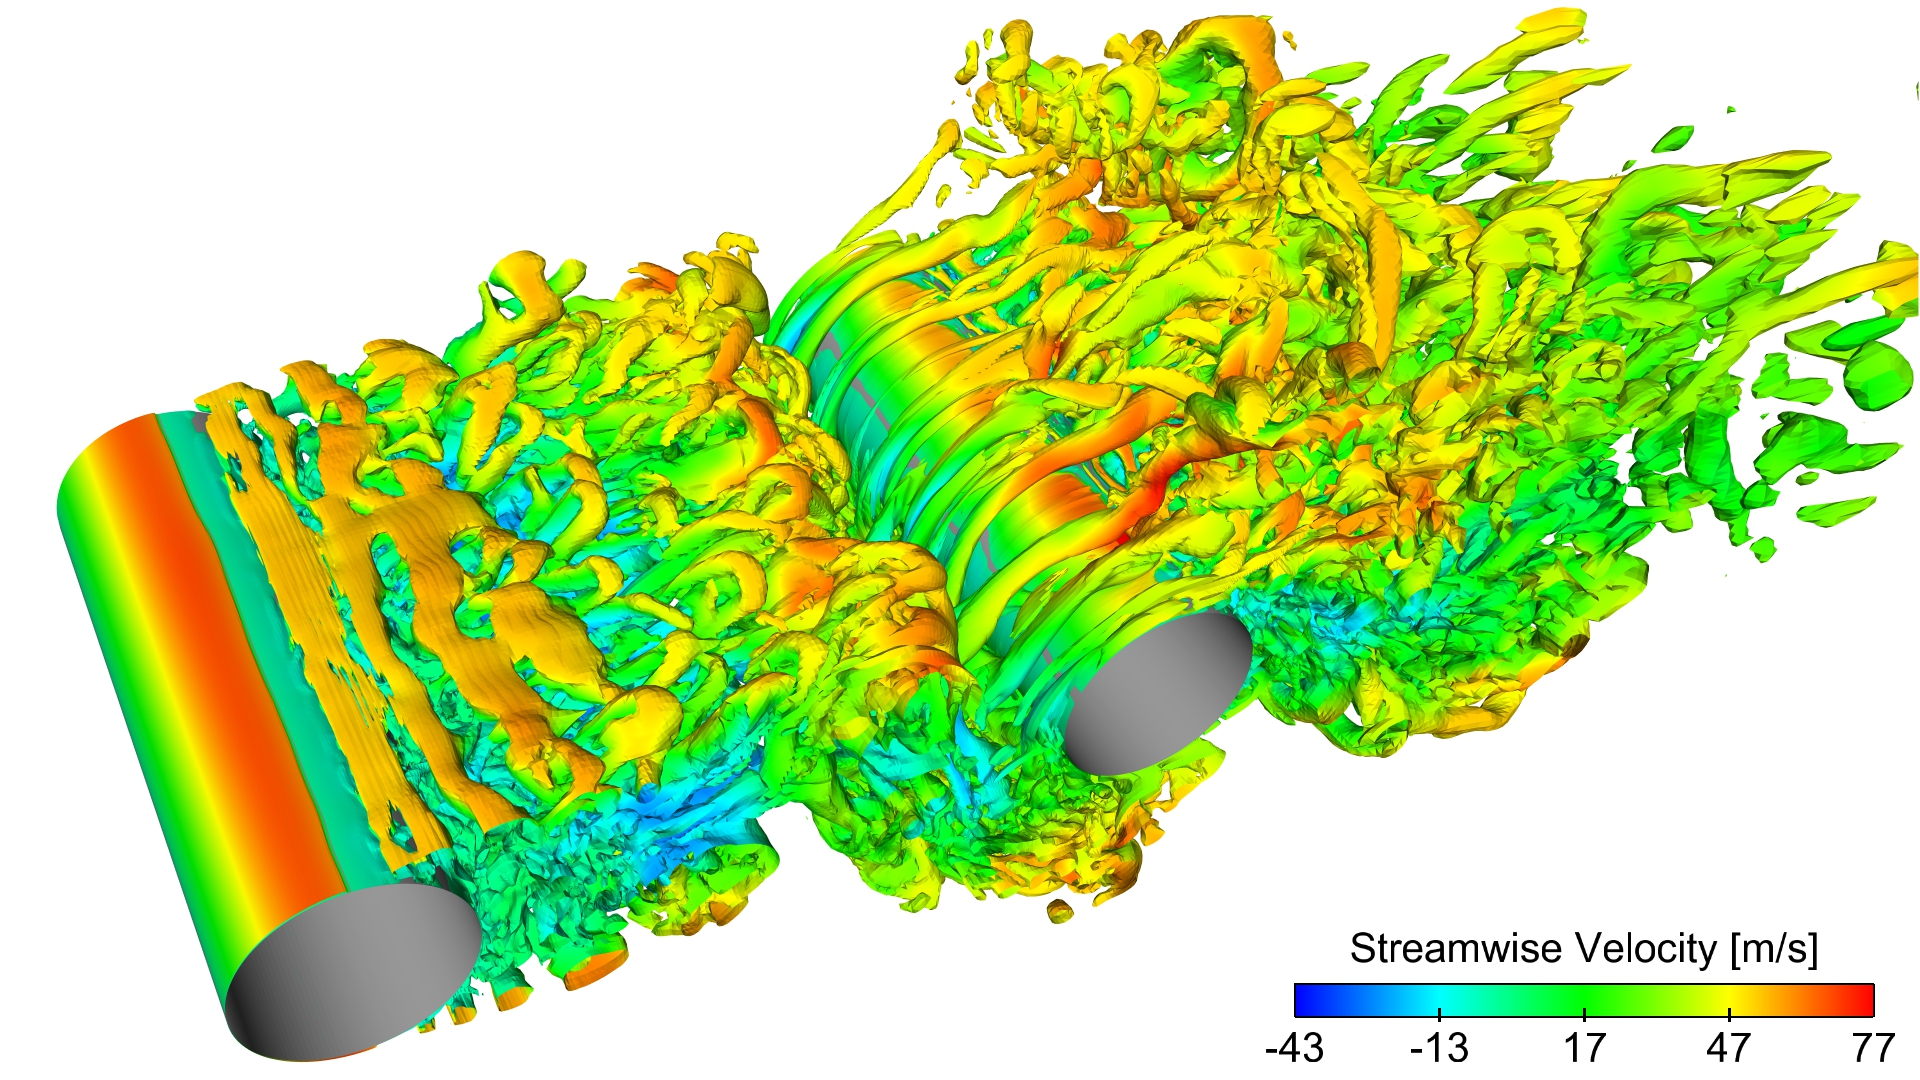
\includegraphics[width=0.40\textwidth]{tc_q_criteria}
    \bicaption{Q判据等值面图,同时测试一下一个很长的标题,比如这真的是一个很长很长很长很长很长很长很长很长的标题。}{Isocontour of Q criteria, at the same time, this is to test a long title, for instance, this is a really very long very long very long very long very long title.}
    \label{fig:tc_q_criteria}
\end{figure}

如果插图的空白区域过大,以图片\verb|shock_cyn|为例,自动裁剪如图\ref{fig:shock_cyn}。
\begin{figure}[!htbp]
    \centering
    %trim option's parameter order: left bottom right top
    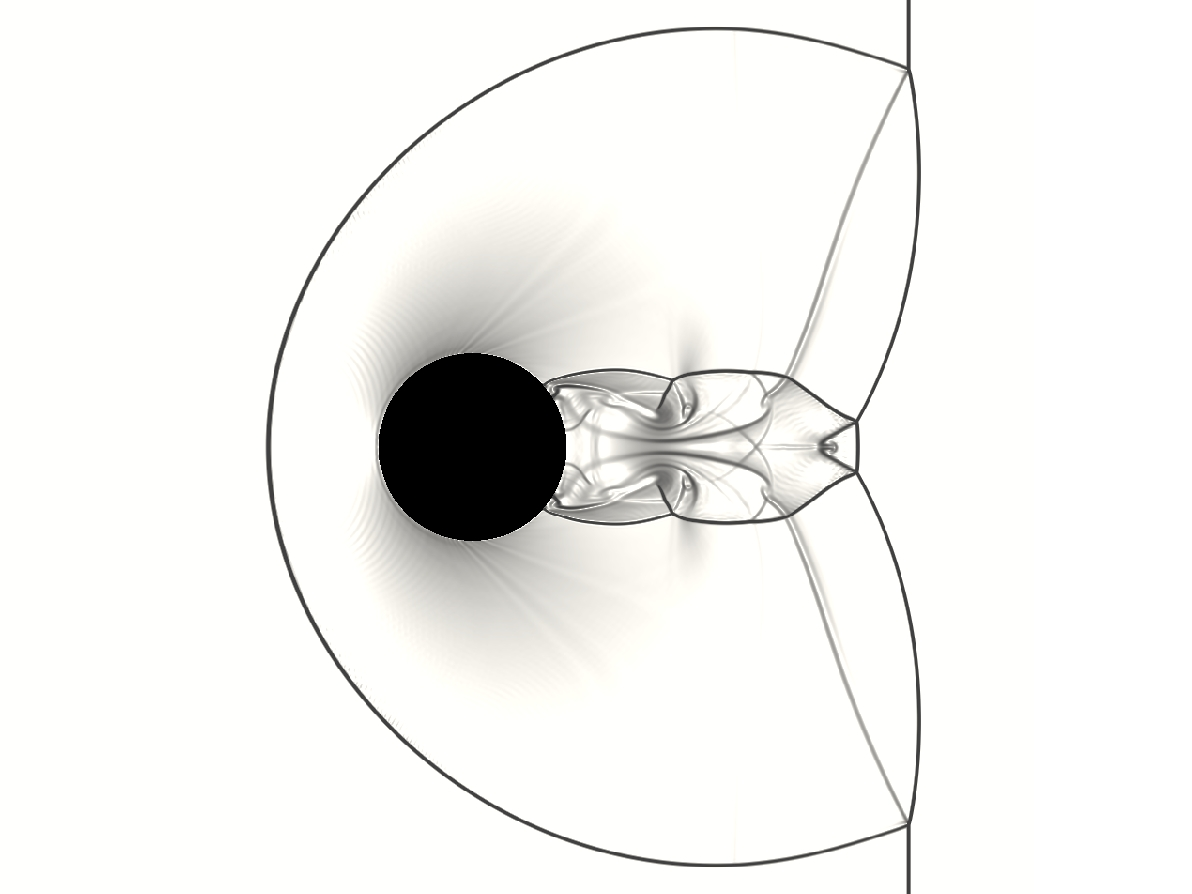
\includegraphics[trim = 30mm 0mm 30mm 0mm, clip, width=0.40\textwidth]{shock_cyn}
    \bicaption{激波圆柱作用。}{Shock-cylinder interaction.}
    \label{fig:shock_cyn}
\end{figure}

多图的插入如图\ref{fig:oaspl},多图不应在子图中给文本子标题,只要给序号,并在主标题中进行引用说明。
\begin{figure}[!htbp]
    \centering
    \begin{subfigure}[b]{0.35\textwidth}
      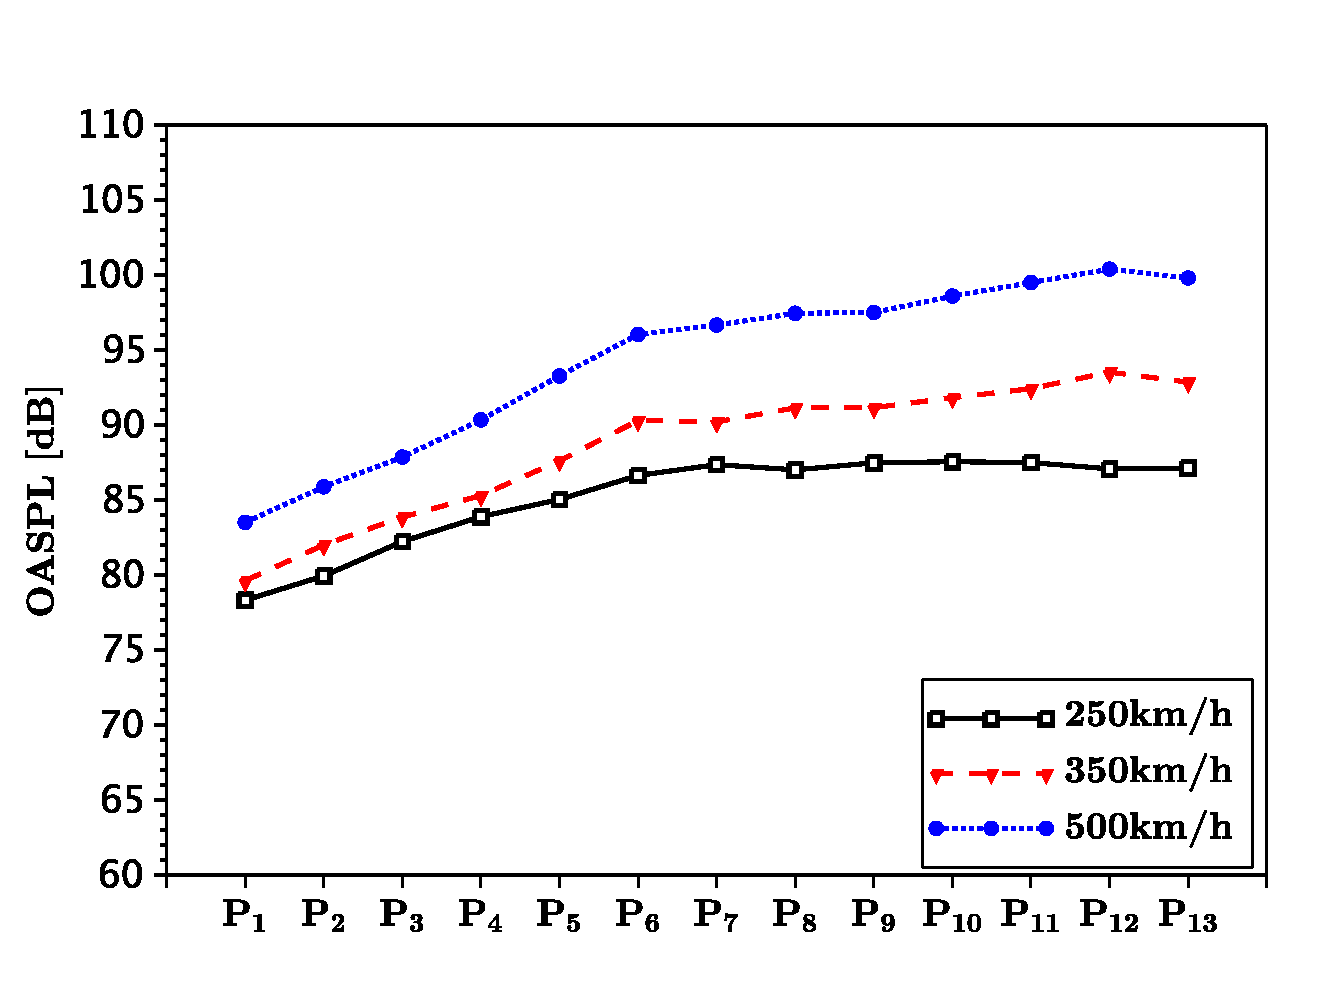
\includegraphics[width=\textwidth]{oaspl_a}
      \caption{}
      \label{fig:oaspl_a}
    \end{subfigure}%
    ~% add desired spacing
    \begin{subfigure}[b]{0.35\textwidth}
      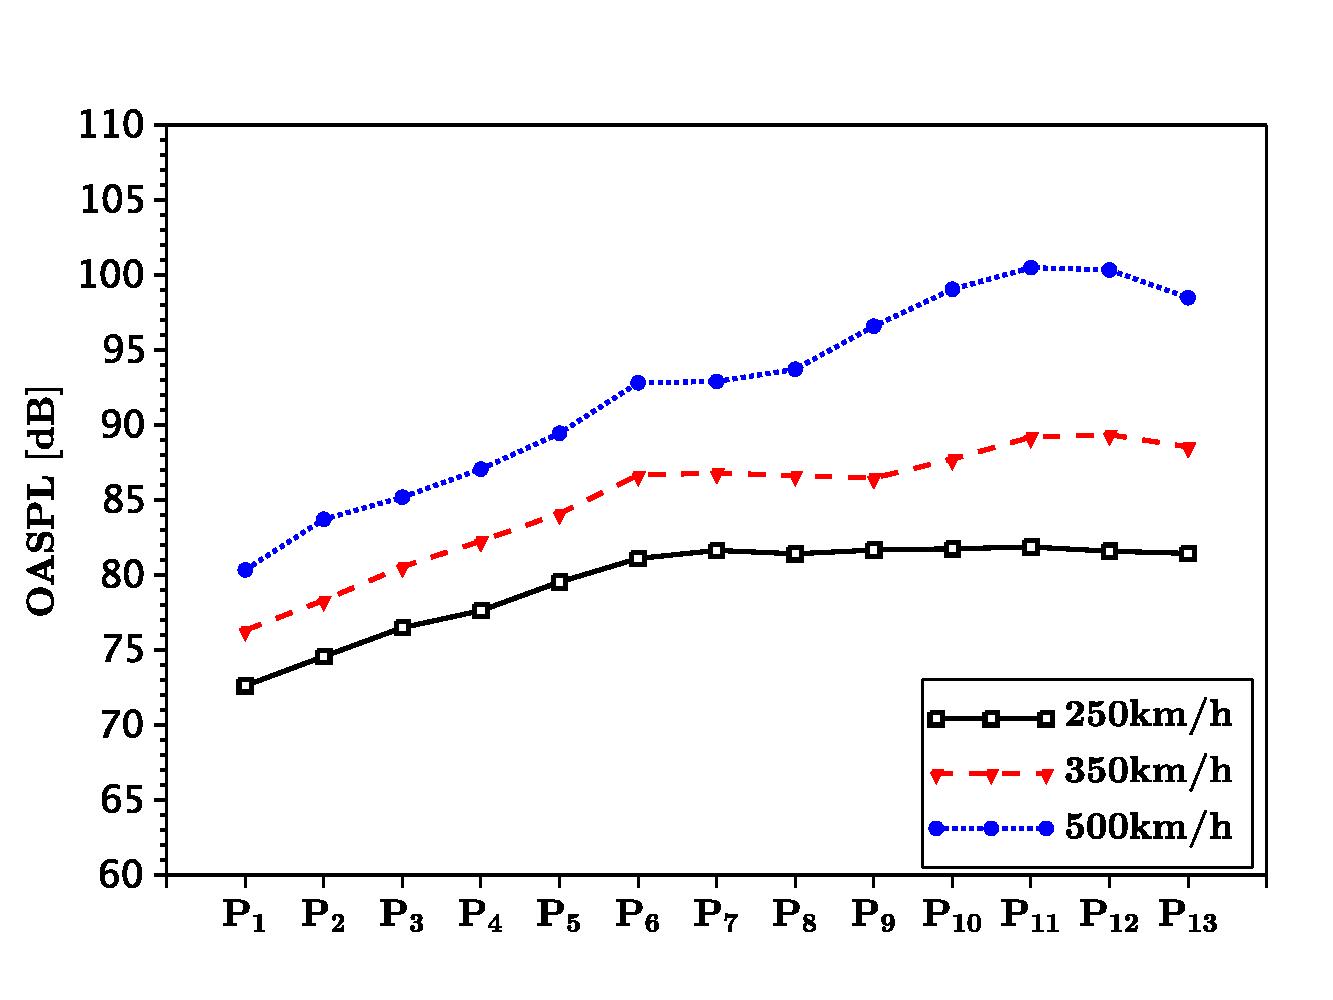
\includegraphics[width=\textwidth]{oaspl_b}
      \caption{}
      \label{fig:oaspl_b}
    \end{subfigure}
    \\% line break
    \begin{subfigure}[b]{0.35\textwidth}
      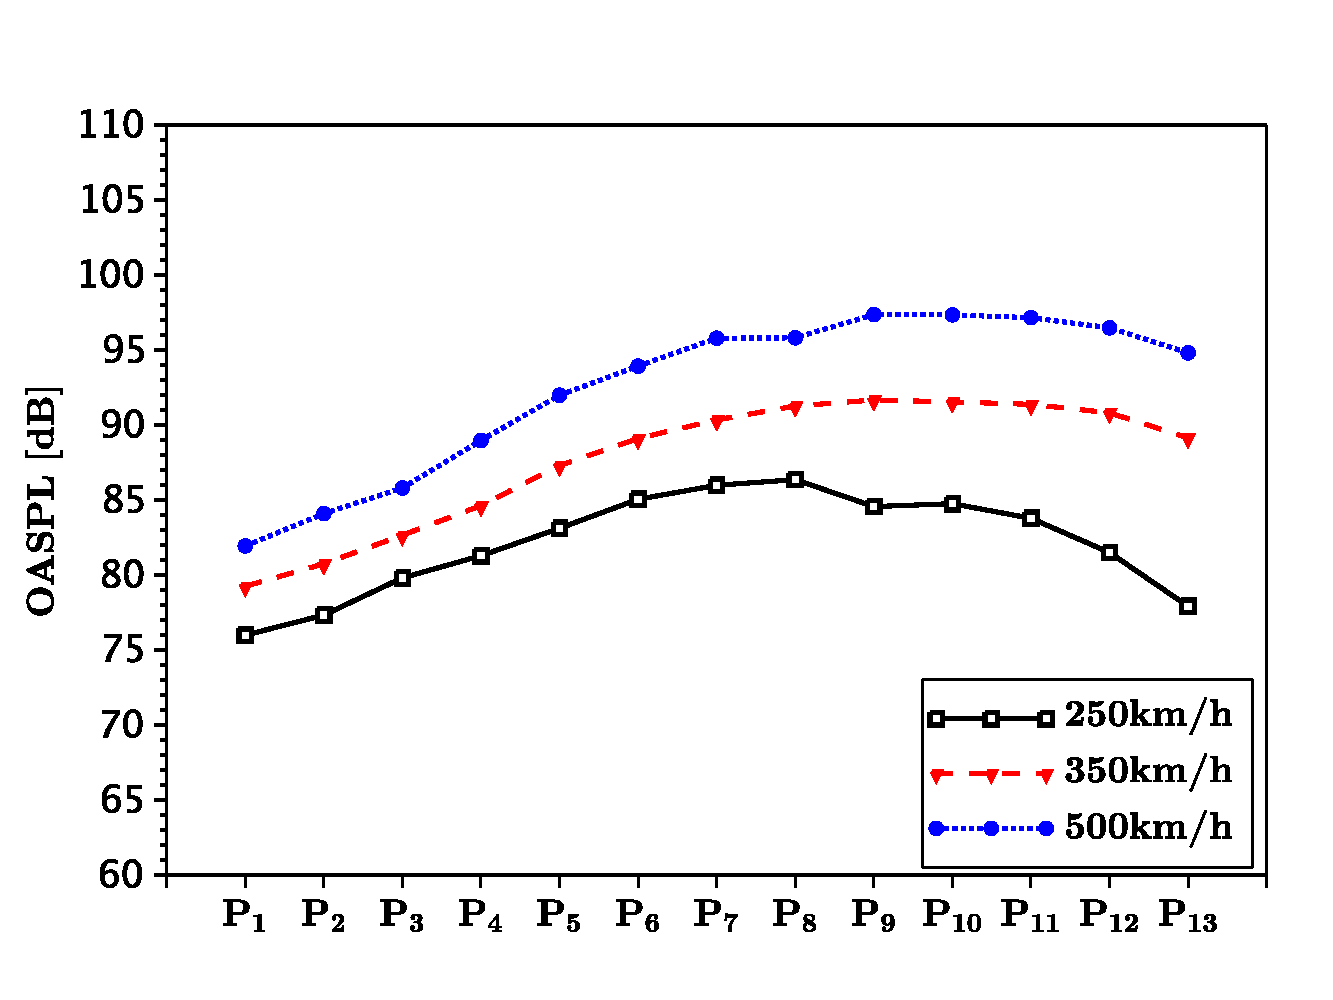
\includegraphics[width=\textwidth]{oaspl_c}
      \caption{}
      \label{fig:oaspl_c}
    \end{subfigure}%
    ~% add desired spacing
    \begin{subfigure}[b]{0.35\textwidth}
      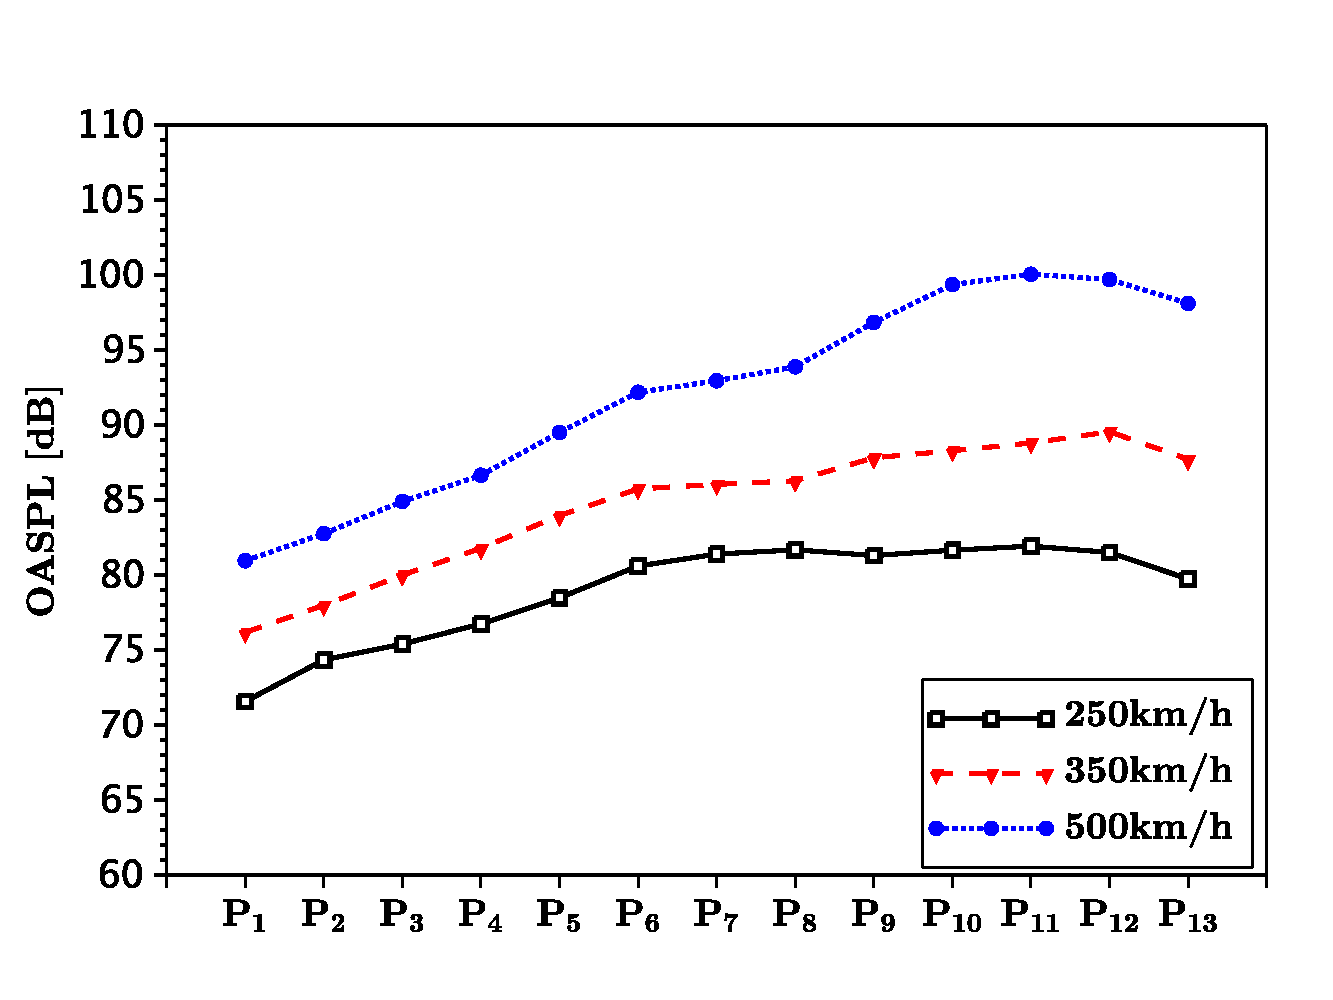
\includegraphics[width=\textwidth]{oaspl_d}
      \caption{}
      \label{fig:oaspl_d}
    \end{subfigure}
    \bicaption{总声压级。(a) 这是子图说明信息,(b) 这是子图说明信息,(c) 这是子图说明信息,(d) 这是子图说明信息。}{OASPL.(a) This is the explanation of subfig, (b) This is the explanation of subfig, (c) This is the explanation of subfig, (d) This is the explanation of subfig.}
    \label{fig:oaspl}
\end{figure}

\subsection{算法}

如见算法~\ref{alg:euclid},详细使用方法请参见文档 \href{https://ctan.org/pkg/algorithmicx?lang=en}{algorithmicx}。

\begin{algorithm}[!htbp]
    \small
    \caption{Euclid's algorithm}\label{alg:euclid}
    \begin{algorithmic}[1]
        \Procedure{Euclid}{$a,b$}\Comment{The g.c.d. of a and b}
        \State $r\gets a\bmod b$
        \While{$r\not=0$}\Comment{We have the answer if r is 0}
        \State $a\gets b$
        \State $b\gets r$
        \State $r\gets a\bmod b$
        \EndWhile\label{euclidendwhile}
        \State \textbf{return} $b$\Comment{The gcd is b}
        \EndProcedure
    \end{algorithmic}
\end{algorithm}

\subsection{参考文献引用}

参考文献引用过程以实例进行介绍,假设需要引用名为"Document Preparation System"的文献,步骤如下:

1)使用Google Scholar搜索Document Preparation System,在目标条目下点击Cite,展开后选择Import into BibTeX打开此文章的BibTeX索引信息,将它们copy添加到ref.bib文件中(此文件位于Biblio文件夹下)。

2)索引第一行 \verb|@article{lamport1986document,|中 \verb|lamport1986document| 即为此文献的label (\textbf{中文文献也必须使用英文label},一般遵照:姓氏拼音+年份+标题第一字拼音的格式),想要在论文中索引此文献,有两种索引类型:

文本类型:\verb|\citet{lamport1986document}|。正如此处所示 \citet{lamport1986document}; 

括号类型:\verb|\citep{lamport1986document}|。正如此处所示 \citep{lamport1986document}。

\textbf{多文献索引用英文逗号隔开}:

\verb|\citep{lamport1986document, chu2004tushu, chen2005zhulu}|。正如此处所示 \citep{lamport1986document, chu2004tushu, chen2005zhulu}

更多例子如:

\citet{walls2013drought} 根据 \citet{betts2005aging} 的研究,首次提出...。其中关于... \citep{walls2013drought, betts2005aging},是当前中国...得到迅速发展的研究领域 \citep{chen1980zhongguo, bravo1990comparative}。引用同一著者在同一年份出版的多篇文献时,在出版年份之后用
英文小写字母区别,如:\citep{yuan2012lana, yuan2012lanb, yuan2012lanc}。同一处引用多篇文献时,按出版年份由近及远依次标注,中间用
分号分开。例如 \citep{chen1980zhongguo, stamerjohanns2009mathml, hls2012jinji, niu2013zonghe}。

使用著者-出版年制(authoryear)式参考文献样式时,中文文献必须在BibTeX索引信息的 \textbf{key} 域(请参考ref.bib文件)填写作者姓名的拼音,才能使得文献列表按照拼音排序。参考文献表中的条目(不排序号),先按语种分类排列,语种顺 序是:中文、日文、英文、俄文、其他文种。然后,中文按汉语拼音字母顺序排列,日文按第一著者的姓氏笔画排序,西文和 俄文按第一著者姓氏首字母顺序排列。如中 \citep{niu2013zonghe}、日 \citep{Bohan1928}、英 \citep{stamerjohanns2009mathml}、俄 \citep{Dubrovin1906}。

如此,即完成了文献的索引,请查看下本文档的参考文献一章,看看是不是就是这么简单呢?是的,就是这么简单!

不同文献样式和引用样式,如著者-出版年制(authoryear)、顺序编码制(numbers)、上标顺序编码制(super)可在Thesis.tex中对artratex.sty调用实现,如:
\begin{itemize}
    \footnotesize
    \item \verb+\usepackage[numbers]{artratex}+ $\%$ 文本: Jones [1]; 括号: [1]
    \item \verb+\usepackage[super]{artratex}+ $\%$ 文本: Jones 上标[1]; 括号: 上标[1]
    \item \verb+\usepackage[authoryear]{artratex}+ $\%$ 文本: Jones (1995); 括号: (Jones, 1995)
    \item \verb+\usepackage[alpha]{artratex}+ $\%$ 文本: 不可用; 括号: [Jon95]
\end{itemize}

当前文档的默认参考文献样式为\textbf{authoryear}。若在上标(\textbf{super})模式下,希望在特定位置将上标改为嵌入式标,可使用

文本类型:\verb|\citetns{lamport1986document,chen2005zhulu}|。

正如此处所示 \citetns{lamport1986document,chen2005zhulu}

括号类型:\verb|\citepns{lamport1986document,chen2005zhulu}|。

正如此处所示 \citepns{lamport1986document,chen2005zhulu}

参考文献索引更为详细的信息,请见 \href{https://en.wikibooks.org/wiki/LaTeX/Bibliography_Management}{WiKibook Bibliography}。\nocite{*}% 使文献列表显示所有参考文献(包括未引用文献)

\section{常见使用问题}\label{sec:qa}

\begin{enumerate}
    \item 模板每次发布前,都已在Windows,Linux,MacOS系统上测试通过。下载模板后,若编译出现错误,则请见 \href{https://github.com/mohuangrui/ucasthesis/wiki}{ucasthesis知识小站} 的 \href{https://github.com/mohuangrui/ucasthesis/wiki/%E7%BC%96%E8%AF%91%E6%8C%87%E5%8D%97}{编译指南}。

    \item 模板文档的编码为UTF-8编码。所有文件都必须采用UTF-8编码,否则编译后生成的文档将出现乱码文本。若出现文本编辑器无法打开文档或打开文档乱码的问题,请检查编辑器对UTF-8编码的支持。如果使用WinEdt作为文本编辑器(\textbf{不推荐使用}),应在其Options -> Preferences -> wrapping选项卡下将两种Wrapping Modes中的内容:
        
        TeX;HTML;ANSI;ASCII|DTX...
        
        修改为:TeX;\textbf{UTF-8|ACP;}HTML;ANSI;ASCII|DTX...
        
        同时,取消Options -> Preferences -> Unicode中的Enable ANSI Format。

    \item 推荐选择xelatex或lualatex编译引擎编译中文文档。编译脚本的默认设定为xelatex编译引擎。你也可以选择不使用脚本编译,如直接使用 \LaTeX{}文本编辑器编译。注:\LaTeX{}文本编辑器编译的默认设定为pdflatex编译引擎,若选择xelatex或lualatex编译引擎,请进入下拉菜单选择。为正确生成引用链接,需要进行全编译。

    \item Texmaker使用简介
        \begin{enumerate}
            \footnotesize
            \item 使用 Texmaker “打开 (Open)” Thesis.tex。
            \item 菜单 “选项 (Options)” -> “设置当前文档为主文档 (Define as Master Document)”
            \item 菜单 “自定义 (User)” -> “自定义命令 (User Commands)” -> “编辑自定义命令 (Edit User Commands)” -> 左侧选择 “command 1”,右侧 “菜单项 (Menu Item)” 填入 Auto Build -> 点击下方“向导 (Wizard)” -> “添加 (Add)”: xelatex + bibtex + xelatex + xelatex + pdf viewer -> 点击“完成 (OK)”
            \item 使用 Auto Build 编译带有未生成引用链接的源文件,可以仅使用 xelatex 编译带有已经正确生成引用链接的源文件。
            \item 编译完成,“查看(View)” PDF,在PDF中 “ctrl+click” 可链接到相对应的源文件。
        \end{enumerate}
    
    \item 模版的设计可能地考虑了适应性。致谢等所有条目都是通过最为通用的

        \verb+\chapter{item name}+  and \verb+\section*{item name}+

        来显式实现的 (请观察Backmatter.tex),从而可以随意添加,放置,和修改,如同一般章节。对于图表目录名称则可在ucasthesis.cfg中进行修改。

    \item 设置文档样式: 在artratex.sty中搜索关键字定位相应命令,然后修改
        \begin{enumerate}
            \item 正文行距:启用和设置 \verb|\linespread{1.5}|,默认1.5倍行距。
            \item 参考文献行距:修改 \verb|\setlength{\bibsep}{0.0ex}|
            \item 目录显示级数:修改 \verb|\setcounter{tocdepth}{2}|
            \item 文档超链接的颜色及其显示:修改 \verb|\hypersetup|
        \end{enumerate}

    \item 文档内字体切换方法:
        \begin{itemize}
            \item 宋体:国科大论文模板ucasthesis 或 \textrm{国科大论文模板ucasthesis}
            \item 粗宋体:{\bfseries 国科大论文模板ucasthesis} 或 \textbf{国科大论文模板ucasthesis}
            \item 黑体:{\sffamily 国科大论文模板ucasthesis} 或 \textsf{国科大论文模板ucasthesis}
            \item 粗黑体:{\bfseries\sffamily 国科大论文模板ucasthesis} 或 \textsf{\bfseries 国科大论文模板ucasthesis}
            \item 仿宋:{\ttfamily 国科大论文模板ucasthesis} 或 \texttt{国科大论文模板ucasthesis}
            \item 粗仿宋:{\bfseries\ttfamily 国科大论文模板ucasthesis} 或 \texttt{\bfseries 国科大论文模板ucasthesis}
            \item 楷体:{\itshape 国科大论文模板ucasthesis} 或 \textit{国科大论文模板ucasthesis}
            \item 粗楷体:{\bfseries\itshape 国科大论文模板ucasthesis} 或 \textit{\bfseries 国科大论文模板ucasthesis}
        \end{itemize}
\end{enumerate}



\chapter{引言}%
\label{chap:introduction}

自从爱因斯坦发现广义相对论以来,人类对宇宙的探索获得了前所未有的理论武器。爱因斯坦在提出广义相对论之后,很快以爱因斯坦方程为基础建立了宇宙学静态模型。1924年弗里德曼发表的文章\citep{friedmann1924moglichkeit}中正式提出了膨胀宇宙模型,基于在爱因斯坦场方程中找到的一个动态解,描述均匀且各项同性宇宙的Friedmann–Lemaître–Robertson–Walker
(FLRW)度规。
1929年哈勃依据对河外星系退行速度的观测数据提出了哈勃定律——遥远星系的退行速度与它们和地球的距离成正比\citep{hubble1929relation}。基于观测数据的哈勃定律提出后,爱因斯坦意识到自己为了获得静态宇宙模型而加入的宇宙学常数$\Lambda$是他“一生中最大的错误”。
在弗里德曼的膨胀宇宙模型以及哈勃定律的基础上,曾出现过各种非主流宇宙模型,例如米尔恩宇宙\citep{milne1936relativity}、弗里德曼提出并由爱因斯坦推广的振荡宇宙、弗里茨$\cdot$兹威基的衰减光子假说\citep{zwicky1929redshift}。
到了40年代,主要有两个基于膨胀宇宙的对立理论。一是由勒梅特提出,乔治$\cdot$伽莫夫支持并完善的热大爆炸理论,另外一个弗雷德$\cdot$霍伊尔等人提出的稳态理论\citep{hoyle1948new}。
伽莫夫在1948年发表的原初核合成理论\citep{alpher1948origin}定量描述了宇宙早期形成的氢元素丰度。另外,伽莫夫的同事拉尔夫$\cdot$阿尔菲和罗伯特$\cdot$赫尔曼从理论上预言了宇宙微波背景辐射(CMB)的存在\citep{alpher1948evolution}。
原初核合成理论的成功以及1964年宇宙微波背景的发现和确认\citep{penzias1965measurement}使得热大爆炸理论胜出。
后来越来越多的实验观测支持存在暗物质\citep{zwicky1933rotverschiebung,zwicky1937masses,clowe2006direct,rubin1980rotational}和暗能量\citep{peebles2003cosmological}。
在热大爆炸理论的基础上加入暗物质和暗能量就得到了现在的标准宇宙学模型,即$\Lambda$CDM模型。$\Lambda$CDM模型包含六个基本参数,能很好的解释宇宙膨胀、宇宙微波背景辐射、宇宙大尺度结构以及物质起源。
但是仍然存在一些根本性问题无法得到解释,如视界疑难\citep{kolb1988early}、平坦性疑难\citep{dicke1979big}等。

为了解决这些问题,Guth\citep{guth1981inflationary}在1981年首次提出了暴胀的概念,认为在宇宙极早期应存在一个短暂的加速膨胀过程,膨胀结束之后直到如今则有标准宇宙学模型进行描述。
在暴胀过程开始之前,目前的整个可观测宇宙都处在一个均匀且各项同性的区域之内。随后在暴胀的作用下,这片区域开始加速膨胀。膨胀的速度是如此之快以至于在暴胀结束之后,这块区域的尺度远远超过了当时的可观测宇宙的尺度。

标准宇宙学模型加上暴胀理论对宇宙演化的描述基本如图$(\ref{fig:history-of-universe})$所描述的样子。

\begin{figure*}[!htbp]
  \centering
  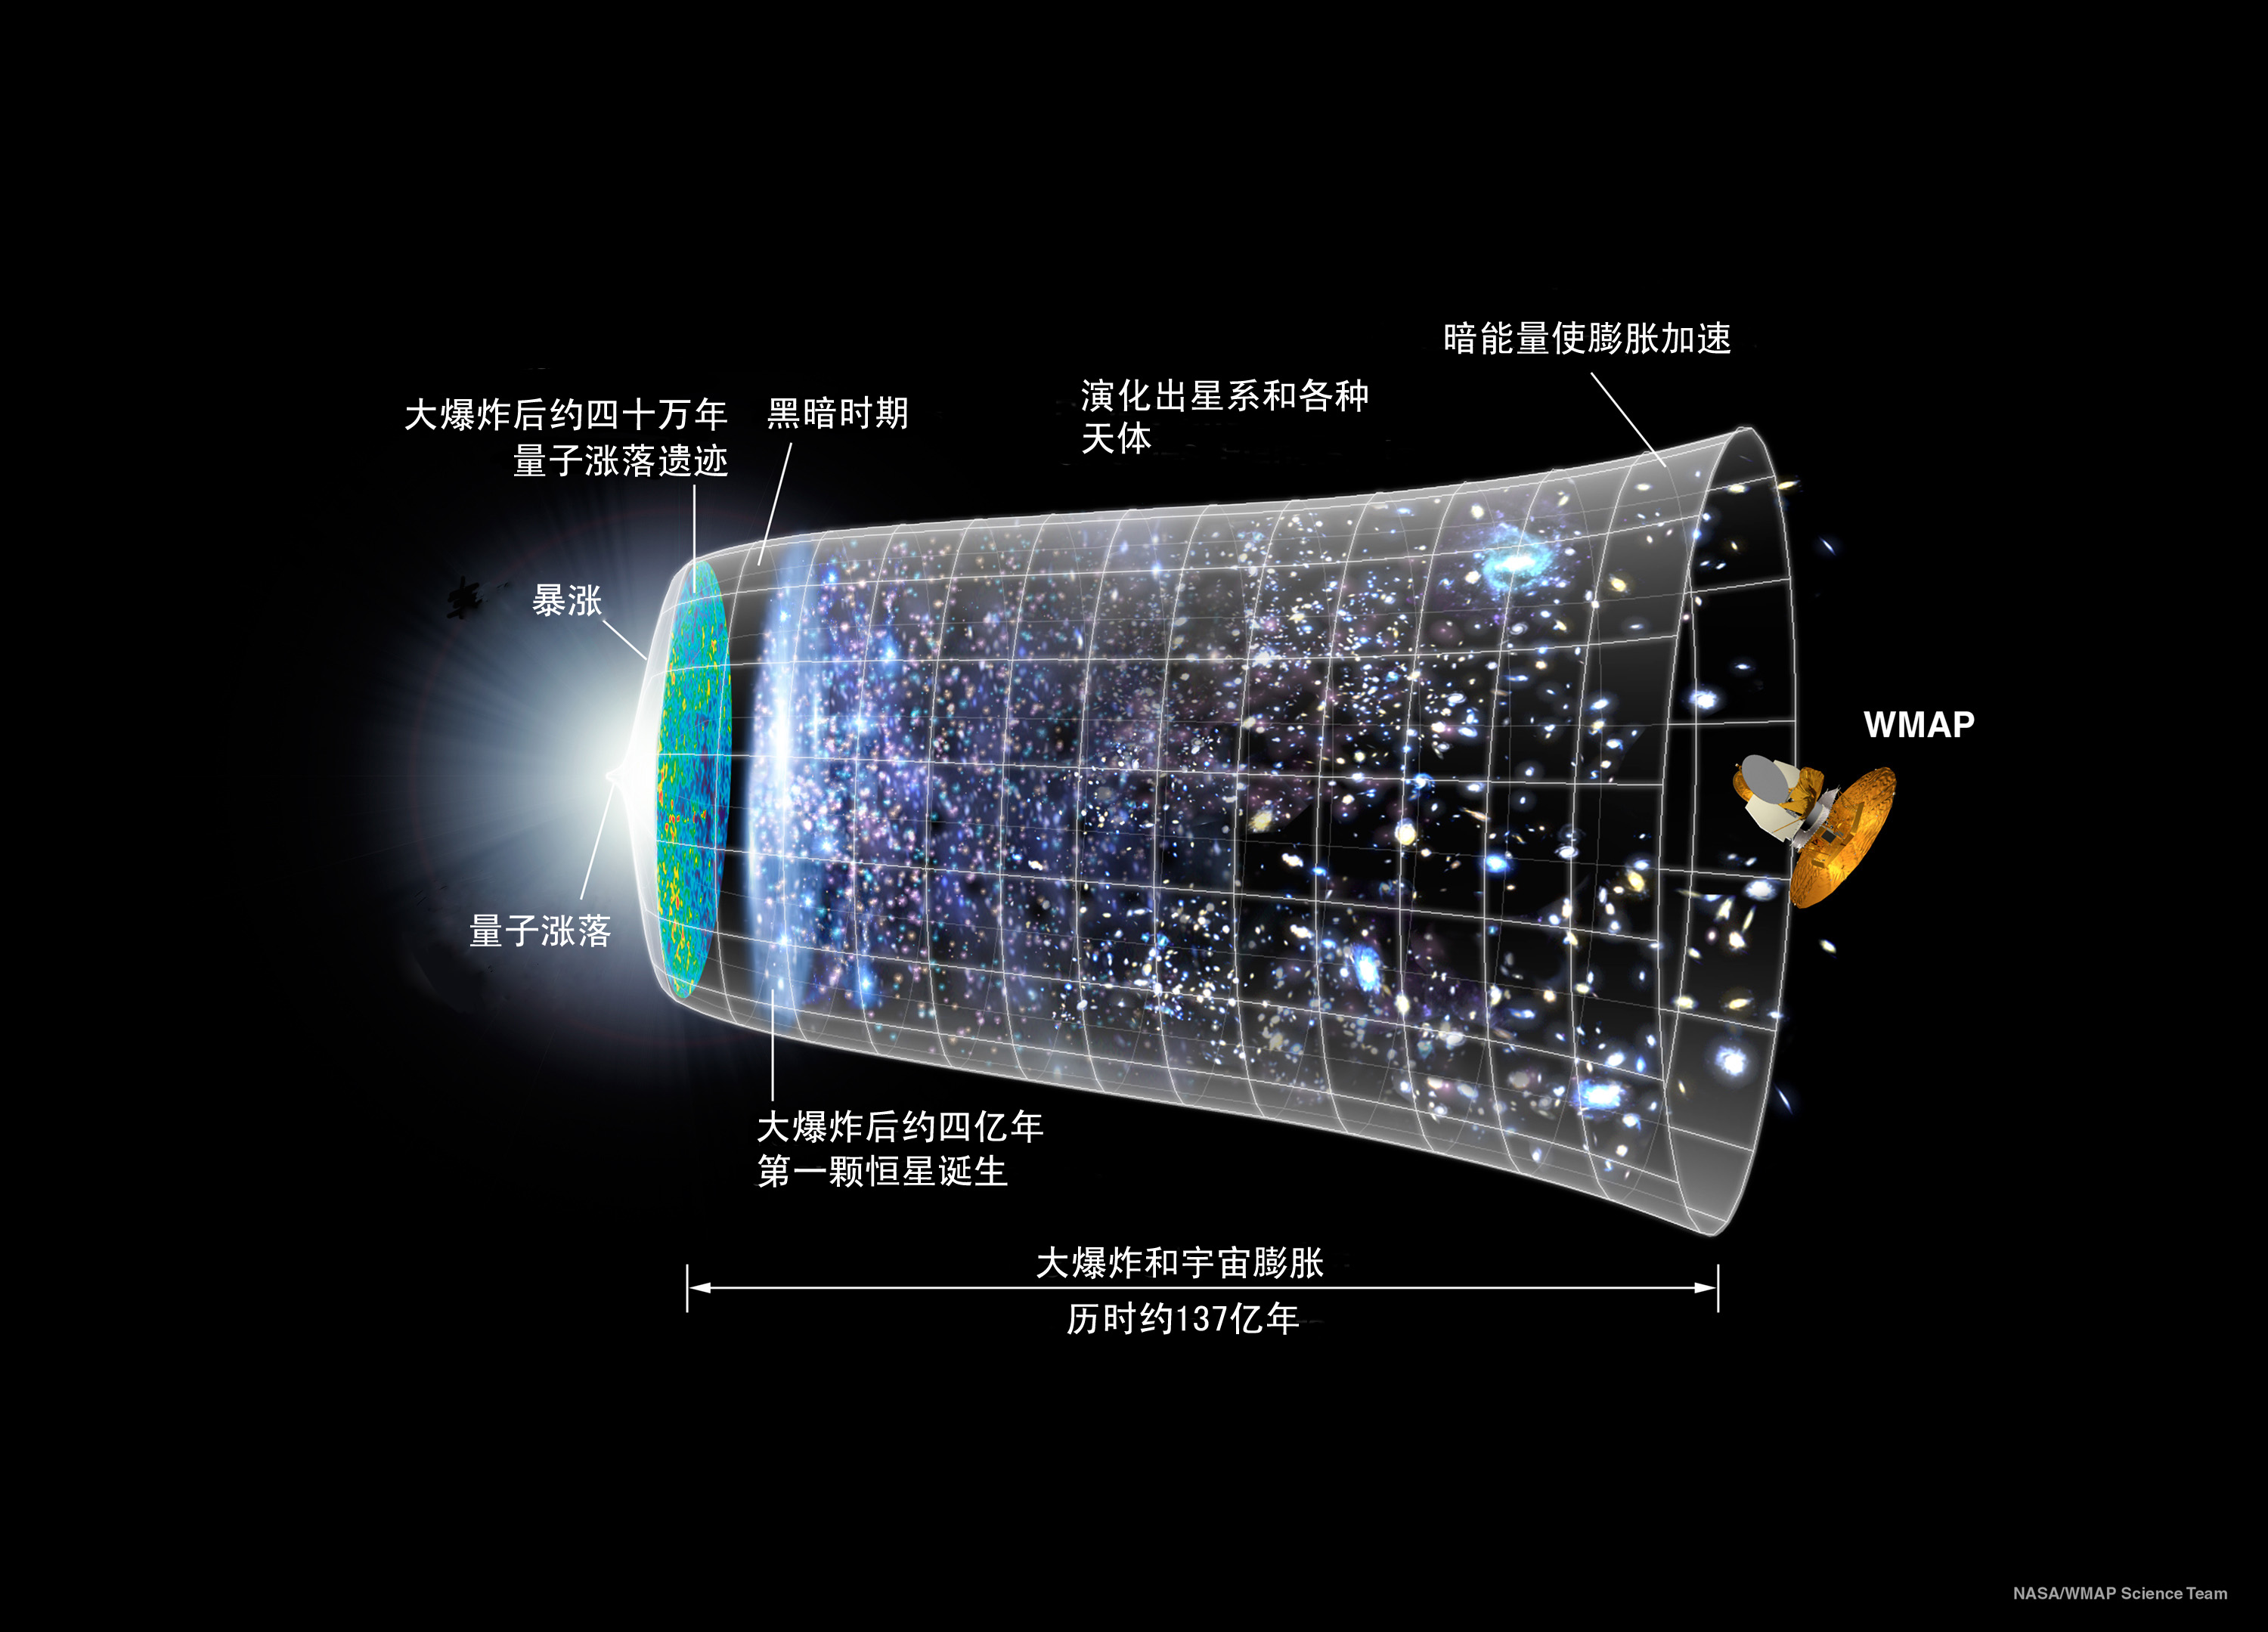
\includegraphics[width=6in]{Img/CMB_Timeline75_zh-cnversion.jpg}
  \caption{宇宙演化的构想图,图片来自2006年WMAP新闻发布会。}\label{fig:history-of-universe}
\end{figure*}

尽管从暴胀的诞生到现在已经有无数个暴胀模型被提出,但是目前为止暴胀的理论起源依旧没有一个统一的结论。
为了尝试给暴胀模型找出背后的理论依据,有人试图把超引力作为一种选择,以其为理论框架,在其中嵌入暴胀模型。超引力暴胀理论到如今已发展了三十多年,各种不同类型的
暴胀模型都已成功在超引力框架内被实现,包括拐点暴胀模型。

暴胀理论还提供了一种产生原初扰动的机制,产生的标量扰动和张量扰动以一种自然的方式解释了CMB中观测到的各项异性以及提供了宇宙大尺度结构能够形成的种子。其中标量扰动的存在已经被CMB各项异性的观测所证实\citep{akrami2018planck}。
大尺度上的张量扰动虽然还未被观测到,但是Planck
2018联合BICEP2/Keck阵列的数据对张标比$r$的上限给出了更紧的限制,在$95\%$的置信水平上$r<0.064$。

一阶扰动理论中,张量扰动满足的运动方程是自由的波动方程。意味着扰动的演化受到宇宙背景演化的直接影响。而在二阶扰动的情况下,自由波动方程获得了一个来自一阶标量扰动的源项\citep{matarrese1998relativistic,acquaviva2002second}。标量扰动在辐射为主时期进入哈勃视界后能够诱导产生二阶引力波。
如果假设标量扰动的功率谱函数是幂指數形式,那么与暴胀期间产生的一阶引力波相比,二阶引力波完全可以被忽略\citep{ananda2007cosmological,baumann2007gravitational},因为根据Planck
2018年的数据,标量谱指标$n_{s}$在$68\%$的置信水平上被限制在$n_{s}=0.9649\pm 0.0042$。
但假若标量功率谱在小尺度上有一个加强的话,二阶引力波的大小甚至可以增大到可以与一阶引力波相比拟,届时便必须考虑它的影响\citep{assadullahi2009gravitational,alabidi2013observable,alabidi2012observable,chen2019pulsar,cai2019gravitational,inomata2019gravitational,cai2019universal}。并且小尺度上功率谱的增强会使得扰动在辐射为主时期进入视界后通过引力塌缩的方式生成原初黑洞\citep{garcia1996density,clesse2015massive,yokoyama1995formation,dalianis2019primordial,gao2018primordial,di2018primordial,garcia2017primordial,garcia2016gravitational}。
因此一阶标量扰动诱导产生的引力波可以用来约束原初黑洞的丰度,反过来原初黑洞的丰度也能用于约束二阶引力波的大小。

此前已经有工作\citep{garcia1702phys}通过单拐点的单场暴胀模型成功使标量谱在小尺度上得到增强。其中用到的拐点暴胀模型是在超引力框架内利用对数K\"ahler势和三次方超势构造得来\citep{gao2015inflection}。近期,又有文章在超引力中基于单手征超场构造出了双拐点暴胀模型\citep{gao2018primordial},其中一个拐点在大尺度上给出满足CMB约束的功率谱,另一个拐点使得功率谱在小尺度上产生一个峰。这个峰的存在使得扰动在辐射为主时期进入视界后能够产生原初黑洞。

基于这个背景,产生了我的第二个工作。在\citep{gao2018primordial}中双拐点暴胀模型的基础上
用解析方法计算二阶诱导引力波的大小,并与LISA和太极的观测灵敏度进行比较,看是否有可能通过诱导引力波的信号是否有可能被探测到。

本文首先将简要介绍现代宇宙学理论,包括标准标准宇宙学、暴胀理论和扰动理论。接下来两章分别介绍整个研究生期间的两个主要工作。文章的具体结构如下。

文章的第二章介绍现代宇宙学标准模型,包括四个部分。第一部分介绍标准宇宙学模型,从宇宙热大爆炸理论到$\Lambda$CDM模型。第二部分介绍暴胀宇宙学,包括历史背景、一般模型以及一些基本概念。
第三部分介绍规范扰动理论,包括扰动的分解、演化以及规范之间的变换。第四部分介绍
扰动功率谱,包括标量扰动以及张量扰动的功率谱的推导。

文章的第三章介绍超引力框架下的单拐点暴胀模型,包括三个部分。第一部分简单介绍了基于超引力的暴胀理论的历史,包括超引力暴胀模型发展过程中遇到的一些问题以及解决方法。第二部分介绍了跑动动能暴胀模型,包含跑动动能暴胀模型提出的背景,以及这一类暴胀模型的基本特点。第三部分介绍了本人的第一个工作,在超引力框架下,
通过选取特定形式的超势$W$,并对参数进行微调得到了具有单个拐点的标量势能。并以
Planck 2015
数据中曲率扰动的大小作为约束条件,计算了多种参数取值下的$n_{s}-r$的预测值,
并将其与 Planck 2015 数据进行了比较,发现与观测较为符合。

文章的第四章介绍了双拐点暴胀模型与引力波,包括四个部分。第一部分介绍了一般的双拐点暴胀模型,及其特点。第二部分首先介绍了超引力下的单场暴胀模型,
然后通过选取满足约束条件的超势构造了一个单场暴胀模型,并且在暴胀结束会得到一个恢复超对称的闵可夫斯基真空。进一步在参数空间中调节超势中引入的几个参数值,将构造出
具有双拐点的暴胀模型。第三部分给出了所构造的双拐点暴胀模型对应的功率谱,由于拐点的
存在,包含慢滚参数的计算功率谱的近似公式将不再适用,因而采用数值方法求解MS方程。
% 第四部分简单介绍原初黑洞,根据原初洞的生成机制以及观测数据,调节功率谱中峰的位置以及幅度。
第四部分根据数值计算得到的标量功率谱计算诱导引力波的能量谱,并将其与LISA\citep{amaro2017laser}和太极\citep{guo2018taiji}的期望灵敏度曲线进行比较。对功率谱进行函数拟合后,对得到的结果进行了一定的推广讨论。
最后一章总结。

\chapter{暴胀}%
\label{chap:inflation}

早在几千年前,人们已经开始仰望星空,未知、好奇、敬畏驱使着他们开始进行力所能及的
观测。然而在很长的一段时间内,我们对宇宙的认识都处在非常局限的状态下。直到文艺
复兴时期,望远镜的发明使得人类获得了第一次技术上的突破,牛顿万有引力定律则是开
启了第一次理论突破,对宇宙的认识开始加剧。直到最近一个多世纪,爱因斯坦的广义相
对论和射电望远镜开启了对宇宙第二波的加速了解。基于广义相对论和宇宙学原理,建立
了现代宇宙学。

\section{标准宇宙学模型}
自1915年爱因斯坦提出广义相对论以来,广义相对论便开始替代牛顿引力理论作为研究宇宙学的理论基础。
时间-空间开始被当作一个整体进行研究,而\textit{爱因斯坦场方程}可以写为
\begin{equation}
    \label{eq:einstein_equation}
    G_{\mu\nu}\equiv R_{\mu\nu}-\frac{1}{2}Rg_{\mu\nu}=T_{\mu\nu},
\end{equation}
其中,$G_{\mu\nu}$为\textit{爱因斯坦张量},$R_{\mu\nu}$和$R$分别为
\textit{里奇张量}和\textit{里奇标量},$T_{\mu\nu}$为\textit{能量-动量张量},
并且约定\textit{约化普朗克质量}$M_p\equiv 1 /\sqrt{8\pi G}=1$。
方程左边代表时空作为一个流形整体的几何性质,右边表示时空中物质的分布情况。
爱因斯坦方程$(\ref{eq:einstein_equation})$说明时空中的物质分布和时空的几何性质之间是互为因果的关系。

为了描述宇宙的演化,首先要确定时空流形的度规以给出方程$(\ref{eq:einstein_equation})$左边的描述。基于当前观测,现代宇宙学普遍采用两条假设作为宇宙学原理:物质分布在宇宙学尺度上是
1)均匀的;2)、各向同性。以此为出发点可以导出用于描述可观测宇宙的
\textbf{弗里德曼-勒梅特-罗伯逊-沃克}(FLRW)度规
\begin{equation}\label{eq:frw_metric}
    ds^2=dt^2-a^2(t)\left[\frac{dr^2}{1-Kr^2}+r^2\left(d\theta^2+\sin^2\theta
    d\phi^2\right)\right],
\end{equation}
其中,$a(t)$为宇宙标度因子,$K>0$,$=0$,$<0$分别代表开放、平直、闭合宇宙。由FLRW度规得到\textit{里奇张量}为
\begin{align}
  R_{00} &= -3\frac{\ddot{a}}{a}, \\
  R_{ij} &= g_{ij}\left(\frac{\ddot{a}}{a}+2H^2+2\frac{K}{a^2}\right), \\
  R_{0i} &= 0,
\end{align}
其中,$H=\dot{a} /a$为哈勃参数,点号表示对宇宙时间$t$的导数。
\textit{里奇标量}为
\begin{equation}
    \label{eq:ricci_scalar}
    R \equiv g^{\alpha\beta}R_{\alpha\beta} =
    6\left(\frac{\ddot{a}}{a}+H^2+\frac{K}{a^2}\right).
\end{equation}
\textit{爱因斯坦张量}
\begin{align}
  \label{eq:einstein_tensor}
  G^{0}_0 &= -3\lrp{H^2+\frac{K}{a^2}}, \\
  G^{0}_i &= 0, \\
  G^i_j &= -\lrp{H^2+ 2 \frac{\ddot{a}}{a}+ \frac{K}{a^2}}.
\end{align}


再看方程右侧,根据宇宙在大尺度上是各向同性且均匀的假设,宇宙可以被近似为理想流体,具有下面的形式的能量-动量张量
\begin{equation}
    \label{eq:energy_moment_tensor}
    T^{\mu}_{\ \nu} =
    \begin{pmatrix}
        \rho & 0 & 0 & 0 \\
        0 & -p & 0 & 0 \\
        0 & 0 & -p & 0 \\
        0 & 0 & 0 & -p
    \end{pmatrix},
\end{equation}
其中$\rho$和$p$分别为能量密度和压强,且只为时间$t$的函数。
根据爱因斯坦方程组中的时间-时间分量和空间-空间分量分别得到如下方程
\begin{align}
    \label{eq:00_einstein} 
    \frac{\dot{a}^2}{a^2} + \frac{K}{a^2} &= \frac{\rho}{3} , \\
    \label{eq:ij_einstein}
    \frac{\ddot{a}}{a}+\frac{2\dot{a}^2}{a^2}+\frac{2K}{a^2}&=
    \frac{\rho-p}{2},
\end{align}
由上面两个方程可以得到两个独立的弗里德曼方程
\begin{align}
    \label{eq:1st_friedmann_equation}
    H^2 &= \frac{\rho}{3}-
    \frac{K}{a^2}, \\
    \label{eq:accelaration_equation}
    \dot{H} + H^2 &= -\frac{\rho+3p}{6}.
\end{align}
由弗里德曼方程可以导出对应能量守恒的连续性方程
\begin{equation}\label{eq:continuation}
    \dot{\rho}=-3H\left(\rho+p\right).
\end{equation}
从方程$(\ref{eq:continuation})$可知宇宙中不同物质的能量密度随时间的演化关系取决于它所服从的物态方程
\begin{equation}
    \label{eq:state_equation}
    p=w\rho,
\end{equation}
其中$w$是物态方程参数,代入连续性方程$(\ref{eq:continuation})$可得
\begin{equation}
    \label{eq:rho_conservation}
    \rho a^{3(1+w)} =\text{常数}.
\end{equation}

对物质和辐射,物态方程参数$w$分别为$0$和$1/3$,因而能量密度$\rho$分别正比于$a^{-3}$和$a^{-4}$。可以看出,辐射的能量密度相比于物质衰减地更快。

$(\ref{eq:energy_moment_tensor})$中能量-动量张量$T_{\mu\nu}$的来源为物质和辐射
。若在场方程中加入宇宙学常数项$\Lambda$,则可以将其移到右侧写作能量-动量张量的
一部分$T^{(vac)}_{\mu\nu}\equiv-\Lambda$,并定义真空能量密度
$\rho_{\text{vac}}\equiv\Lambda$。对真空能,物态方程参数$w=-1$,根据方程
$(\ref{eq:rho_conservation})$真空能不随时间衰减。从这里开始分别以$\rho_r,\
\rho_m,\ \rho_{\Lambda}$表示辐射、物质和真空能的能量密度。

由于宇宙中各组分的能量密度的衰减速率不一,使得占据宇宙能量密度主导地位的组分在
宇宙演化的不同时期并不相同。根据各组分的衰减速率,宇宙将先后由辐射、物质和真空
能占据主导地位,决定宇宙的演化方式。在各个时期,标度因子$a(t)$随时间的变化关系为
\begin{equation}
    a(t)\propto 
    \begin{cases}
      t^{1/2},\qquad &\text{辐射为主}\\
      t^{2/3},\qquad &\text{物质为主}\\
      e^{\sqrt{\Lambda/3}t},\qquad &\text{真空为主}
    \end{cases}
\end{equation}
严格意义上宇宙的总能量密度$\rho_{tot}$应为真空、物质和辐射三部分的和
\begin{equation}
    \rho_{tot} = \rho_{\Lambda}+\rho_m+\rho_r,
\end{equation}
为了确定宇宙在三维空间上的几何性质(正曲率闭合空间、负曲率开放空间还是零曲率平直空间),定义临界能量密度 
\begin{equation}
    \label{eq:critical_rho}
    \rho_{cr} = 3H^2,
\end{equation}
于是弗里德曼方程$(\ref{eq:1st_friedmann_equation})$变成
\begin{equation}
    \rho_{cr}\left(1 + \frac{K}{a^2H^2}\right) = \rho_{tot}.
\end{equation}
再引入无量纲参数 $\Omega_{tot}\equiv
\rho_{tot}/\rho_{cr}$,空间曲率 $K$可以表示成
\begin{equation}\label{eq:flatness}
    \Omega - 1 = \frac{K}{a^2H^2} ,
\end{equation}
对宇宙微波背景辐射的观测支持$K$接近于$0$,故我们认为当前所处的宇宙在空间上是平
直的,没有曲率。从这里开始若无特别说明,均假定$K=0$。
在平直宇宙中,各组分的密度参数之和为一
\begin{equation}
    \Omega_{\Lambda}+\Omega_m+\Omega_r=1.
\end{equation}
于是在任意时刻,由弗里德曼方程$(\ref{eq:1st_friedmann_equation})$给出标度因子$a(t)$满足的方程
\begin{equation}
    \frac{\dot{a}}{a} =
    H_0\sqrt{\Omega_{\Lambda,0}+\frac{\Omega_{m,0}}{a^3}+\frac{\Omega_{r,0}}{a^4}},
\end{equation}
其中,$\Omega_{\Lambda,0}$、$\Omega_{m,0}$、$\Omega_{r,0}$分别表示暗能量、
物质以及辐射的密度参数在当前时刻的值。

\section{双拐点暴胀模型}

拐点暴胀模型简介

双拐点暴胀模型引入

双拐点暴胀模型特点

拐点暴胀通常指这样的暴胀模型,存在场值$\phi=\phi_0$(拐点)使得势能在该处的二阶导数为零
\begin{equation}
    V^{\dprime}(\phi_0) = 0
\end{equation}

势能的一般形式为

\begin{equation}
    \label{eq:inf_potential}
    V (\phi)=V_0+a (\phi-\phi_0)+\frac{c}{6}{\left(\phi-\phi_0\right)}^3\\
\end{equation}
\begin{equation}
    V_0\equiv V (\phi_0),\ a\equiv V' (\phi_0),\ c\equiv V^{\tprime} (\phi_0) 
\end{equation}

高阶项 $(n \geq 4)$ 被截断。相应的慢滚参数为
\begin{equation}
    \label{eq:psrp}
    \epsilon = \frac{M_p}{2}\left(\frac{V'}{V}^2\right),\ \eta=M^2_p
    \left(\frac{V^{\dprime}}{V}\right),\ \xi^2=M^4_p\left(\frac{V'V^{\tprime}}{V^2}\right)
\end{equation}

接下来通过WMAP、Planck等实验观测到的标量扰动大小$\mathcal{P}_R$和标量谱指标$n_s$来确定系数a和c。
令暴胀结束时的场值为$\phi_e$,那时有$\epsilon\sim
1$。则对应$\phi\sim\phi_e$的e-folding数为
\begin{align}
    \label{eq:e-folding}
    \mathcal{N} &= \frac{V_0}{M^2_p}\sqrt{\frac{2}{ac}}\lbrack
    F_0(\phi_e)-F_0(\phi)\rbrack \\
    F_0(z) &= \cot^{-1}\left(\sqrt{\frac{c}{2a}}(z-\phi_0)\right)
\end{align}

如果将慢滚参数在极值处的平方根定义为 $X$, $\mathcal{N}$ 中涉及 $\phi$
的部分定义为 $Y$,那么可以将各慢滚参数及可观测量用统一用$X,Y$进行描述。

\begin{align}
    \epsilon &=
    \frac{2V_0^2}{c^2M_p^6\mathcal{N}^4} {\left(\frac{Y}{X} \right)}^4 \\
    \eta &=
    -\frac{2}{\mathcal{N}}\frac{Y}{S}\left(\sqrt{1-X}\cos Y-\sqrt{X}\sin
    Y\right)\\
    \xi^2 &= \frac{2}{\mathcal{N}^2}{\left(\frac{Y}{X}\right)}^2
\end{align}

在暴胀期间,$\epsilon \ll 1$,导致$X=S\sqrt{\epsilon}\leq\sqrt{\epsilon}\ll
1$,故而有$S\approx \sin Y$。相应的功率谱,标量谱指标及其跑动为
\begin{align}
    \mathcal{P}^{1/2}&\equiv\frac{1}{\sqrt{24\pi^2}}\frac{V_0^{1/2}}{\epsilon^{1/2}M_p^2}
    \approx\frac{V_0^{1/2}}{2\sqrt{6}\pi M_p^2 X}\sin^2Y\\
    n_s&\equiv1+2\eta-6\epsilon\approx1-\frac{4}{\mathcal{N}}Y\cot Y\\
\end{align}

\section{暴涨}
由于共动距离不随时间改变,在共动坐标系下讨论\textbf{(共动)粒子视界}会使视界问
题变得更简单。若标度因子$a(t)$是时间$t$的幂函数,则在当前时刻$t_0$和过去某一时刻$t_1$的因果联系区的共动尺度比为
\begin{align}
  \frac{\chi_{p 0}}{\chi_{p 1}}\sim \frac{t_0}{t_1}\frac{a_1}{a_0}
  \sim \frac{\dot{a}_1}{\dot{a}_0}.
\end{align}

平坦性问题中,给大爆炸宇宙学造成困难的地方来自于比值
\begin{align}
  \label{eq:flatness-of-space}
  \frac{\Omega_0-1}{\Omega_1-1}=
  \frac{{\left(Ha\right)}^2_{1}}{{\left(Ha\right)}^2_{0}}
  \sim {\left(\frac{\dot{a}_1}{\dot{a}_0}\right)}^2.
\end{align}
在这几个问题中,都出现了比值$\dot{a}_1 /
\dot{a}_0$。当强能量条件满足时$\rho+3p>0$,根据加速度方程
$(\ref{eq:accelaration_equation})$标度因子的二阶导数小于零,因此宇宙处于减速
膨胀的状态。故越早期,比值$\dot{a}_1 /\dot{a}_0$越大,问题越严重。如果要求
$\dot{a}_1 /\dot{a}_0\leq 1$,那么只能假设$\dot{a}$经历了先增大、后渐小的过程。
引入的这一段加速膨胀的过程是必要的,至于是否充分取决于实现这一条件的特定模型。
根据加速度方程,普通物质的存在提供了引力使得宇宙的膨胀速度减小。那么为了实现
加速膨胀,必须假设宇宙中存在别的物质,使得引力表现为一种“排斥力”。

我们先给出暴涨的定义:\textbf{暴涨}是当引力表现为一种排斥力使得宇宙处于加速膨胀的一个阶段。

暴涨能够解释大爆炸的起源。因为加速膨胀,原本处于因果联系区内的一个小区域会在短时间内膨胀地非常大。更进一步,
暴涨甚至能从一个均匀的小区域中产生整个可观测宇宙,即便这一区域外相当非均匀。原因在于,在一个加速膨胀的宇宙中,
总是存在有限大的事件视界
\begin{align}
    d_{e}(t) &= a(t)\int_t^{t_{\text{max}}} \frac{dt}{a}
    =a(t)\int_{a(t)}^{a_{\text{max}}} \frac{da}{\dot{a}a}\notag \\
    &= \sqrt{3}a(t)\int_{a(t)}^{a_{\text{max}}}
    \frac{da}{a\sqrt{a^{-(1+3w)}-3K}}.
\end{align}
因为${\left(1+3w\right)}<0$,即使$a_{\text{max}}\rightarrow
\infty$,$d_{e}(t)$也会收敛到有限值。如此一来,以$
p$为中心,$d_{e}(t)$为半径的区域$V_1(t)=\{q\ |\
|q-p|<d_{e}(t)\}$其未来的演化永远不会受到来自于半径为$2d_{e}(t)$的同心区域$V_2(t)$外的影响。能对内部产生作用的只有半径在$d_{e}(t)$到$2d_{e}(t)$的部分。假设在$t=t_{i}$时$V_2(t_{i})$内部的物质分布均匀且各向同性,那么到暴涨结束时,$V_1(t_{f})$内始终保持均匀和各向同性。$V_1(t)$区域的物理尺度在暴涨结束时为
\begin{align}
  d_{e}(t_{f})=d_e(t_{i}) \frac{a_{f}}{a_{i}}.
\end{align}
在加速膨胀宇宙中,粒子视界可以作如下近似
\begin{align}
  d_{p}(t) =a(t)\int_{t_{i}}^{t} \frac{dt}{a}=a(t)\int_{a_{i}}^{a}
  \frac{da}{\dot{a}a}\sim \frac{a(t)}{a_{i}}d_{e}(t_i). 
\end{align}
因为积分的主要贡献来自于$a\sim a_{i}$的部分。在暴涨结束时,$d_{p}(t)\sim
d_{e}(t)$,说明均匀区域的大小与粒子视界的尺度相当。不同于一个均匀的宇宙包含很多不同的因果关联区,我们可以从一个
很小的均匀的因果关联区出发,通过暴涨使得它的大小以爆炸似的方式变大,同时保持了均匀性。

下一个问题是\textbf{均匀性}的条件是否可以放开,即不要求暴涨开始时因果关联区内部物质分布的均匀性。那么我们
从一个高度非均匀的因果关联区出发,计算一下暴涨结束时的扰动大小。假设初始的相对
能量密度扰动在$\sim
H_{i}^{-1}$的尺度上为$\mathcal{O}(1)$的量级,
\begin{align}
  {\left(\frac{\delta \rho}{\rho}\right)}_{t_{i}}
  \sim \frac{1}{\rho} \frac{|\nabla\rho|}{a_{i}}H_{i}^{-1}
  =\frac{|\nabla\rho|}{\rho}\frac{1}{\dot{a}_{i}}
  \sim \mathcal{O}(1),
\end{align}
这里$\nabla$是在共动坐标系中对空间的导数。当$t\gg
t_{i}$时,哈勃半径$H^{-1}(t)$内的能量密度扰动近似为
\begin{align}
  \label{eq:relative-energy-density-perturbation}
  {\left(\frac{\delta\rho}{\rho}\right)}_{t}
  \sim \frac{1}{\rho} \frac{|\nabla\rho|}{a(t)}H^{-1}(t)
  \sim \mathcal{O}(1) \frac{\dot{a}_{i}}{\dot{a}(t)}.
\end{align}

这里假设了$|\nabla\rho|/\rho$不会在暴涨期间产生明显变化。这一假设的合理性可以来自于对标量扰动在大于$H^{-1}$的尺度上的行为的分析。
$(\ref{eq:relative-energy-density-perturbation})$说明当宇宙处于加速膨胀过程中时,在半径为$H^{-1}$的区域内,
相对能量密度扰动会变得越来越小。因而宇宙变得越来越平坦。

总结起来,如今我们观测到的均匀且各向同性的宇宙,可以有一个非均匀的起源,只要存在暴涨就可以将非均匀性给抹除。

同时,暴涨也能解决平坦性问题。从$(\ref{eq:relative-energy-density-perturbation})$可以发现,如果要求避免大的密度扰动重新进入视界($\sim
H_0^{-1}$)使得宇宙的均匀性假设被破坏,那么必须假设暴涨开始时候的膨胀率远小于今天的膨胀率,即$\dot{a}_{i}/\dot{a}_0\ll
1$。
再精确一点,可以根据CMB的观测要求在当今的视界尺度上,能量密度扰动的方差不应当超过$10^{-5}$。
只要满足条件$\dot{a}_{i}/\dot{a}_0\ll
10^{-5}$,方程$(\ref{eq:relative-energy-density-perturbation})$即可被满足,暴涨时的非均匀性足够被抹除。
$(\ref{eq:flatness-of-space})$可以改写为
\begin{align}
  \Omega_0=1+{\left(\Omega_{i}-1\right)}{\left(\frac{\dot{a}_{i}}{\dot{a}_0}\right)}^2.
\end{align}
可以看出只要满足条件$|\Omega_{i}-1|\sim\mathcal{O}(1)$,就能使得
\begin{align}
  \Omega_0=1.
\end{align}
在相当高的精度上成立。还可以从另一个角度来理解,在减速膨胀的宇宙中,只当$t\rightarrow
0$时会有$\Omega(t)\rightarrow
1$。而在加速膨胀的宇宙中,是当$t\rightarrow\infty$时才有$\Omega(t)\rightarrow
1$。因而只要在减速膨胀阶段之前存在一个加速膨胀阶段,困扰我们的精细调节问题便不复存在。



一般我们通过标量场来实现一个强能量条件$(\rho+3p >
0)$被破坏的模型,相应的场被称为暴涨场。带有暴涨势$V(\varphi)$的标量场$\varphi$的能动量张量为
\begin{align}
  \label{eq:scalar-energy-momentum-tensor}
  T^{\alpha}_{\ \beta} = \varphi^{,\alpha}\varphi_{,\beta}-
  \frac{1}{2}{\left(\varphi^{,\gamma}\varphi_{,\gamma}-V(\varphi)\right)}\delta^{\alpha}_{\
  \beta}.
\end{align}
根据$T^{\alpha}_{\ \beta;\alpha}=0$可得
\begin{align}
  \varphi^{;\alpha}_{\ ;\alpha}+V_{,\varphi}
  =0,
\end{align}
能动量张量$T^{\alpha}_{\
\beta}$可以改写为理想流体的能动量张量形式,
\begin{align}
  \label{eq:perfect-fluid-energy-momentum-tensor}
  T^{\alpha}_{\ \beta}=(\rho+p)u^{\alpha}u_{\beta}-p\delta^{\alpha}_{\
  \beta}.
\end{align}
若$\varphi^{,\gamma}\varphi_{,\gamma}>0$,且
\begin{align}
  \rho &= \frac{1}{2}\varphi^{,\gamma}\varphi_{,\gamma}+V(\varphi),\\
  p&= \frac{1}{2}\varphi^{,\gamma}_{,\gamma}-V(\varphi), \\
  u^{\alpha}&= \varphi^{,\alpha}/
  \sqrt{\varphi^{,\gamma}\varphi_{,\gamma}},
\end{align}
特别当$\varphi$场是均匀场,即$\partial\varphi /\partial x^{i}=0$时场的能量密度为
\begin{equation}\label{eq:energy_density}
  \rho = \frac{1}{2}\dot{\varphi}^2+V(\varphi),
\end{equation}
以及压强
\begin{equation}\label{eq:pressure}
  p=\frac{1}{2}\dot{\varphi}^2-V(\varphi).
\end{equation}
相应的连续性方程$(\ref{eq:continuation})$
以及弗里德曼方程$(\ref{eq:1st_friedmann_equation})$改写为
\begin{equation}
  \label{eq:continuation_in_inflation}
  \ddot{\varphi}+3H\dot\varphi+V_{,\varphi}=0,
\end{equation}
\begin{equation}
  \label{eq:1st_friedmann_equation_in_inflation}
  3H^2=\frac{1}{2}\dot\varphi^2+V(\varphi).
\end{equation}
% 约定约化普朗克质量$M_p\equiv\frac{1}{\sqrt{8\pi G}}=1$。
消去标量场$\varphi$的二阶导数,得到Hamilton-Jacobi方程
\begin{align}
  \lbrack H_{,\varphi} \rbrack^2 - H^2 &=
  -V(\varphi)\label{HJa}, \\
  \dot\varphi  &= -2H_{,\varphi} \label{HJb}.
\end{align}

由$(\ref{HJb})$可知$\dot H=-\dot \varphi^2 /2\leq 0$,故物理哈勃半径$1/H$
随时间增大。同时标度因子$a(t)$加速增大,故共动哈勃半径$1/(aH)$不断随时间减小。
方程$(\ref{HJa})$有一个很好的性质,即任意一个方程解的线性扰动都会以指数的速度趋于零,因此很容易进行数值求解。

因为$\rho+3p=2{(\dot{\varphi}^2-V(\varphi))}$,所以只有当$\dot{\varphi}^2<V(\varphi)$时,宇宙才能加速膨胀。
而在常见的慢滚暴涨模型中,假设动能项远小于势能项,$\dot{\varphi}\ll
V(\varphi)$,并且摩擦项$3H\dot{\varphi}$足够大,使得加速度项$\ddot{\varphi}$迅速减小直至可被忽略。
基于慢滚暴涨模型的上述两个假设,方程$(\ref{eq:continuation_in_inflation})$及$(\ref{eq:1st_friedmann_equation_in_inflation})$简化为
\begin{align}
  \label{eq:friedmann_equation_in_slow_roll_inflation}
  3H\dot{\varphi} &= -V_{,\varphi} , \\
  3H^2&=V(\varphi).
\end{align}
为了更好地刻画与描述慢滚暴涨过程,通常借助慢滚参数。慢滚参数有两种定义方式,基于暴涨势和哈勃参数的慢滚参数(SRP)。
分别以下标V和H表示,定义势能慢滚参数
\begin{align}
  \label{eq:PSRA_epsilon}
  \epsilon_V(\varphi) &= \frac{1}{2}
  {\left(\frac{V_{,\varphi}}{V(\varphi)}\right)}^2,
  \\
  \label{eq:PSRA_eta}
  \eta_V(\varphi) &= \frac{V_{,\varphi \varphi}}{V(\varphi)}.
\end{align}
及哈勃慢滚参数
\begin{align}
  \label{eq:HSRA_epsilon}
  \epsilon_H(\varphi) &= 2
  {\left(\frac{H_{,\varphi}}{H(\varphi)}\right)}^2=-\frac{\dot{H}}{H^2}, \\
  \label{eq:HSRA_eta}
  \eta_H(\varphi) &= 2 \frac{H_{,\varphi \varphi}}{H(\varphi)}=-3
  \frac{\ddot{\varphi}}{3H\dot{\varphi}}.
\end{align}
相比$\epsilon_V$和$\eta_V$,采用$\epsilon_H$和$\eta_H$描述暴涨的优势在于
\begin{itemize}
  \item $\epsilon_H\ll 1$是动能项相比于势能项可被忽略的充要条件。\\
  \item $\lvert \eta_H\rvert \ll
    1$是加速度项相比于摩擦项可被忽略,不需要额外假设存在吸引子解的充要条件。
    因此哈勃SRP中包含了所有必要的动力学信息。 \\
  \item 暴涨发生的充要条件为
    \begin{equation}
      \ddot{a} > 0 \Longleftrightarrow \epsilon_H < 1. 
    \end{equation}
\end{itemize}



% 能够退出暴涨是一个暴涨模型有效的必要条件之一。假设$H^2$比$\dot{H}$变化的更快,则暴涨持续的时间根据$(\ref{eq:accelaration_equation})$可得
% \begin{align}
%   \label{eq:time_for_inflation}
%   t_f \sim H_i/\lvert H_i\rvert,
% \end{align}
% 为了保证不出现平坦性疑难,暴涨结束时需满足条件
% \begin{align}
%    \frac{a_{f}}{a_{i}} > 10^{33}\frac{H_{i}}{H_{f}},
% \end{align}
% 假设$\lvert H_{i}\rvert \ll
% H^2_{i}$且哈勃参数不随时间变化,则由上式可得估计
% \begin{align}
%   \frac{\lvert\dot{H_i}\rvert}{H^2_i} < \frac{1}{75},
% \end{align}
% 假设$k=0$,利用上式可以得到初始状态方程满足的约束条件
% \begin{align}
%   \frac{\rho_i+p_i}{\rho_i} < 10^{-2}. 
% \end{align}
% 换言之,暴涨开始时对真空物态方程的偏离不超过$1\%$.

\section{CMB和标量扰动}

宇宙学原理假设其中之一是宇宙在大尺度结构上是均匀且各向同性。但真实情况是存在一个一阶扰动修正,扰动可以非均匀、各向异性。带有扰动的弗里德曼平坦宇宙的度规为
\begin{align}
  \label{eq:perturbation-metric}
  ds^2=\left[^{(0)}g_{\alpha\beta}+\delta g_{\alpha\beta}(x^{\gamma})
  \right]dx^{\alpha}dx^{\beta},
\end{align}
其中$|\delta g_{\alpha\beta}|\ll|^{(0)}g_{\alpha\beta}|$。采用共动时间时,
背景度规为
\begin{align}
  \label{eq:background-metric}
  ^{(0)}g_{\alpha\beta}=a^2(\eta)\text{diag}(1, -1, -1, -1).
\end{align}
度规扰动$\delta
g_{\alpha\beta}$可以分解为三种类型:\textbf{标量扰动}、\textbf{矢量扰动}和\textbf{张量扰动}。
三种扰动独立演化,互不影响。
扰动$\delta g_{\alpha\beta}$的来源之一,是
从物理角度,仅仅因为坐标变换导致的扰动不是真实的扰动。而在坐标变换下的不变量才是反映真实扰动的物理量,
这样的不变量称为\textbf{规范不变量}。以时空为变量的无穷小函数$\xi^{\alpha}(x)$,可以用来定义一个无穷小坐标变换。
\begin{align}
  \label{eq:coordinate-transformation}
  x^{\alpha} \rightarrow \tilde{x}^{\alpha}=x^{\alpha}+\xi^{\alpha}.
\end{align}
4-标量$q(x^{\rho})$的扰动$\delta
q=q(x^{\rho})-^{(0)}q(x^{\rho})$按如下方式变换
\begin{align}
  \label{eq:scalar-perturbation-transformation}
  \delta q \rightarrow \delta\tilde{q}=\delta q
  -^{(0)}q_{,\alpha}\xi^{\alpha}.
\end{align}
同理可知4-矢量扰动和4-张量扰动的变换规则为
\begin{align}
  \label{eq:vector-perturbation-transformation}
  \delta u_{\alpha} \rightarrow \delta\tilde{u}_{\alpha}&=
  \delta
  u_{\alpha}-^{(0)}u_{\alpha,\gamma}\xi^{\gamma}-^{(0)}u_{\gamma}\xi^{\gamma}_{,\alpha},
  \\
  \label{eq:tensor-perturbation-transformation}
  \delta g_{\alpha\beta}\rightarrow\delta \tilde{g}_{\alpha\beta} &=
  \delta g_{\alpha\beta}-^{(0)}g_{\alpha\beta,\gamma}\xi^{\gamma}
  -^{(0)}g_{\gamma\beta}\xi^{\gamma}_{,\alpha}-^{(0)}g_{\alpha\gamma}\xi^{\gamma}_{,\beta}.
\end{align}

考虑标量扰动时,度规的最一般形式为
\begin{align}
  \label{eq:scalar-metric-perturbation}
  g_{\alpha\beta}=a^2(\eta)
  \begin{pmatrix}
    1 + 2\phi & B_{,j} \\
    B_{,i} & -(1-2\psi)\delta_{ij}+E_{,ij}
  \end{pmatrix}
\end{align}

其中$\phi$,$\psi$,$B$,$E$为3-标量。
根据扰动的规范变换,可得这几个标量函数相应的变换规则。通过观察发现有这些标量函数的线性组合可得的最简单的
规范不变量有两个,分别为
\begin{align}
  \label{eq:gauge-invariant-scalar}
  \Phi\equiv \phi -\frac{1}{a}{[a{\left(B-E^{\prime}\right)}]}^{\prime}
  ,\qquad
  \Psi \equiv \psi + \frac{a^{\prime}}{a}{\left(B-E^{\prime}\right)}.
\end{align}
容易验证$\Phi$和$\Psi$在坐标变换下不变,包含了真实的扰动信息。

同理,



\chapter{超引力中的单拐点暴胀模型}%
\label{chap:inflection_model}

\section{拐点暴胀模型基本概念}
\section{双拐点暴胀模型}
拐点暴胀通常指这样的暴胀模型,存在场值$\phi=\phi_0$(拐点)使得势能在该处的二阶导数为零
\begin{equation}
    V^{\dprime}(\phi_0) = 0
\end{equation}

势能的一般形式为

\begin{equation}
    \label{eq:inf_potential}
    V (\phi)=V_0+a (\phi-\phi_0)+\frac{c}{6}{\left(\phi-\phi_0\right)}^3\\
\end{equation}
\begin{equation}
    V_0\equiv V (\phi_0),\ a\equiv V' (\phi_0),\ c\equiv V^{\tprime} (\phi_0) 
\end{equation}

高阶项 $(n \geq 4)$ 被截断。相应的慢滚参数为
\begin{equation}
    \label{eq:psrp}
    \epsilon = \frac{M_p}{2}\left(\frac{V'}{V}^2\right),\ \eta=M^2_p
    \left(\frac{V^{\dprime}}{V}\right),\ \xi^2=M^4_p\left(\frac{V'V^{\tprime}}{V^2}\right)
\end{equation}

接下来通过WMAP、Planck等实验观测到的标量扰动大小$\mathcal{P}_R$和标量谱指标$n_s$来确定系数a和c。
令暴胀结束时的场值为$\phi_e$,那时有$\epsilon\sim
1$。则对应$\phi\sim\phi_e$的e-folding数为
\begin{align}
    \label{eq:e-folding}
    \mathcal{N} &= \frac{V_0}{M^2_p}\sqrt{\frac{2}{ac}}\lbrack
    F_0(\phi_e)-F_0(\phi)\rbrack \\
    F_0(z) &= \cot^{-1}\left(\sqrt{\frac{c}{2a}}(z-\phi_0)\right)
\end{align}

如果将慢滚参数在极值处的平方根定义为 $X$, $\mathcal{N}$ 中涉及 $\phi$
的部分定义为 $Y$,那么可以将各慢滚参数及可观测量用统一用$X,Y$进行描述。

\begin{align}
    \epsilon &=
    \frac{2V_0^2}{c^2M_p^6\mathcal{N}^4} {\left(\frac{Y}{X} \right)}^4 \\
    \eta &=
    -\frac{2}{\mathcal{N}}\frac{Y}{S}\left(\sqrt{1-X}\cos Y-\sqrt{X}\sin
    Y\right)\\
    \xi^2 &= \frac{2}{\mathcal{N}^2}{\left(\frac{Y}{X}\right)}^2
\end{align}

在暴胀期间,$\epsilon \ll 1$,导致$X=S\sqrt{\epsilon}\leq\sqrt{\epsilon}\ll
1$,故而有$S\approx \sin Y$。相应的功率谱,标量谱指标及其跑动为
\begin{align}
    \mathcal{P}^{1/2}&\equiv\frac{1}{\sqrt{24\pi^2}}\frac{V_0^{1/2}}{\epsilon^{1/2}M_p^2}
    \approx\frac{V_0^{1/2}}{2\sqrt{6}\pi M_p^2 X}\sin^2Y\\
    n_s&\equiv1+2\eta-6\epsilon\approx1-\frac{4}{\mathcal{N}}Y\cot Y\\
\end{align}

\section{一些拐点暴胀模型的文章}
这里我们讨论如何在超引力中构建一个拐点暴胀模型。基于超引力构建的大多数旧暴胀模型\citep{freedman1989progress,deser1976consistent,wess1992supersymmetry}都遇到了$\eta$问题\citep{yamaguchi2011supergravity}:F-term势能正比于指数因子$e^{|\phi|^2}$,使得慢滚参数$\eta$不满足慢滚条件。有多种方法可以$\eta$问题\citep{stewart1995inflation,linde1994hybrid,linde1997hybrid,panagiotakopoulos1997hybrid}。其中一种办法是将平移对称性引入K\"ahler势中$K(\phi-\phi^\dagger)$,这样暴胀子不会出现在K\"ahler势中,消失的指数因子保证了势能的平坦性。这种情形下,能够得到幂指数势能$V(\phi)\propto
\phi^n$的混沌暴胀。

有作者\citep{takahashi2010linear,nakayama2010running,kasuya2014flat}将手征场$\phi$的类Nambu-Goldstone平移对称性推广到了一般形式$\phi^n\rightarrow
\phi^n+C$,使得K\"ahler势是$\left(\phi^n-\phi^\dagger\right)$的函数。
为了获得合理的势能形式,应当在K\"{a}hler势和超势中分别加入一个小的shift对称性破缺项$\kappa|\phi|^2$和$\lambda\phi^m
X$,此处有$\kappa,\lambda\ll
1$以及外场$X$。这样可以获得幂指数为分数的标量势能$V(\phi)\propto
\phi^{m/n}$,标量谱指标$n_s$以及张标比$r$近似为
$n_s=1-(1+\frac{m}{n})\frac{1}{N}$和$\frac{8m}{n}\frac{1}{N}$\citep{nakayama2010running}。
由于模型中动能项的系数是场依赖的:$(\kappa+n^2|\phi|^{2n-2})\partial_{\mu}\phi\partial^{\mu}\phi^{\dag}$,这就是所谓的跑动动能项暴胀。

在最小超对称标准模型的框架下,通过规范不变的平坦方向\textit{udd}或\textit{LLe}首次构造出了拐点暴胀模型\citep{allahverdi2006gauge},并得到了发展\citep{allahverdi2007term,enqvist2010inflection,hotchkiss2012observable,chatterjee2015bound}。
在\citep{gao2015inflection}中,作者用单手征超场构造出了一个拐点暴胀模型,与Planck
2015年的结果相一致。在暴胀结束后,该模型进入一个非超对称德-西特真空,能够用于解释宇宙近期的加速膨胀。

\subsection{带跑动动能项的多项式超势}
K\"ahler势在手征超场$\phi$的广义平移对称性变换下保持不变:
\begin{equation}
    \phi^n \rightarrow \phi^n + C,
\end{equation}

因此,它必然是$i\chi \equiv (\phi^n - \phi^{n\dagger})$的函数:
\begin{equation}
    K = \sum_{l=1}\frac{c_l}{l}{\left(\phi^n-\phi^{n\dagger}\right)}^l
    =
    i c_1(\phi^n-\phi^{n\dagger})-\frac{1}{2}{\left(\phi^n-\phi^{n\dagger}\right)}^2+\cdots.
\end{equation}

系数$c_l$是与$1$同量级的常数。在暴胀期间,$\chi$一直稳定在极小值处,所以$l\ge
3$的项对动能的贡献可以忽略\citep{takahashi2010linear}。对$l\le2$的项,$\chi$稳定在$\chi_{\text{min}}\simeq
c_1$。

为了使暴胀模型可行,需要在K\"ahler势中添加一个微小的平移对称性破缺项:
\begin{equation}
    \Delta{K} = \kappa \left|\phi\right|^2,
\end{equation}
系数满足条件$0< \kappa \ll 1$。

与\citep{nakayama2010running}不同,我们假设超势满足一个更一般的形式\citep{nakayama2013polynomial,kawasaki2000natural,kawasaki2001natural,kallosh2010new,kallosh2011general}
\begin{equation}
    W = X\left(\sum_{m=0}\lambda_m\phi^m\right)+W_0.
\end{equation}
这里$\lambda_m\ll
1$,$X$是一个额外的手征超场,并且稳定在$X=0$。$\left|W_0\right|\simeq
m_{3/2}$且$m_{3/2}$为引力微子的质量。按照通常的假设,在暴胀过程中$m_{3/2}$远远小于哈勃参数,所以在讨论暴胀动力学的时候可以被丢弃。

所以最终的K\"ahler势为
\begin{equation}
    K = \kappa |\phi|^2 + c_1(\phi^n-\phi^{n\dagger}) -
    \frac{1}{2}{(\phi^n-\phi^{n\dagger})}^2 + |X|^2\cdots.
\end{equation}

超势$W$和K\"ahler势共同决定了标量场$\phi$的有效拉式量
\begin{equation}
\begin{split}\label{eq:lagrangian}
L &= -K^{\phi\phi^\dagger} \partial_\mu\phi\partial^\mu\phi^\dagger
- V \\
  & = (\kappa + n^2|\phi|^{(2n-2)})
  \partial_\mu \phi \partial^\mu \phi^\dagger - V,
\end{split}
\end{equation}
暴胀场$\phi$的标量势能为
\begin{equation}
\begin{split}
V &= e^K \left[
    D_\phi W{(K^{-1})}^{\phi\phi^\dagger}{(D_\phi W)}^{\star} - 3|W|^2 
    \right]\\
  &=
  e^{\kappa|\phi|^2+c_1(\phi^n-\phi^{n\dagger})-\frac{1}{2}{(\phi^n-\phi^{n\dagger})}^2}{(\sum_m
  \lambda_m|\phi|^m)}^2,
\end{split}
\end{equation}
其中
\begin{equation}
    D_\phi W = \partial_\phi W + (\partial_\phi K) W,
\end{equation}
以及
\begin{equation}
    K^{\phi\phi^\dagger} = \frac{\partial^2 K}{\partial\phi
    \partial\phi^\dagger}
\end{equation}

当${(\kappa/n^2)}^{1/(2n-2)}\ll |\phi| \ll
\kappa^{-1/2}$时,$\kappa$项可以忽略,所以若定义$\hat{\phi} \equiv
\phi^n$,则意味着$\hat{\phi}$在类Nambu-Goldstone平移变换下不变,拉式量
(\ref{eq:lagrangian})近似为
\begin{equation}
\begin{split}
    L &= \partial_\mu \hat{\phi}\partial^\mu \hat{\phi}^\dagger -
    e^{-\frac{|c_1|^2}{2}}{(\sum_m \lambda_m|\hat{\phi}|^{m/n})}^2 \\
    &= \partial_\mu \hat{\phi} \partial^\mu \hat{\phi}^\dagger - 
    {(\sum_m \hat{\lambda_m}|\hat{\phi}|^{m/n})}^2,
\end{split}
\end{equation}
其中$i\chi \equiv (\phi^n - \phi^{n\dagger})=i c_1$,$\hat{\lambda}_m\equiv
e^{-\frac{|c_1|^2}{4}}\lambda_m$。

由于平移对称性,$\hat{\phi}$的实部不会出现在K\"ahler势中,所以势能在实方向上相当地平坦使得其成为暴胀子候选者。
虚部获得了比哈勃能标更重地质量,并且在暴胀过程中稳定在极小值处。因此,设$\hat{\phi}\equiv
(\varphi+i \chi)/\sqrt{2}=\varphi/\sqrt{2}+i
c_1/2$并得到$\varphi$地标量势能
\begin{equation}\label{eq:varphi_scalar_potential}
    V = {\left[\sum_{m=0}\hat{\lambda}_m
    {\left(\frac{\varphi}{\sqrt{2}}\right)}^{\frac{m}{n}}\right]}^2.
\end{equation}

\subsection{建立拐点暴胀模型}
为了创建一个拐点暴胀模型,我们采用如下形式的超势
\begin{equation}\label{eq:superpotential}
    W = X(\lambda_p\phi^p + \lambda_q e^{i\theta}\phi^q),
\end{equation}
其中幂指数$q > p \le
1$且为整数,系数$\lambda_p$、$\lambda_q$为正实数且不失一般性,$\theta$为第二项的相位。

将 (\ref{eq:superpotential})代入势能函数
(\ref{eq:varphi_scalar_potential})得到
\begin{equation}
\begin{split}
    V &= {\left[ \hat{\lambda}_p {\left(\frac{\varphi}{\sqrt{2}}\right)}^{\frac{p}{n}}
    + \hat{\lambda}_q e^{i\theta}{\left(\frac{\varphi}{\sqrt{2}}\right)}^{\frac{q}{n}}\right]}^2 \\
    &= \hat{\lambda}_p^2 {\left(\frac{\varphi}{\sqrt{2}}\right)}^{\frac{2p}{n}}
    \left[1 + 2\xi\cos\theta {\left(\frac{\varphi}{\sqrt{2}}\right)}^{\frac{q-p}{n}}
    + \xi^2 {\left(\frac{\varphi}{\sqrt{2}}\right)}^{\frac{2(q-p)}{n}}\right],
\end{split}
\end{equation}
其中$\hat{\lambda}_{p,q}\equiv
e^{-\frac{|c_1|^2}{4}}\lambda_{p,q}$和$\xi=|\hat{\lambda}_q/\hat{\lambda}_p|=|\lambda_q/\lambda_p|$。
% 势能曲线参见图\ref{fig:varphi_scalar_potential}。

% \begin{figure}
%     \centering
%     \includegraphics{}
%     \caption{暴胀势能$V(\phi)$,其中$\cos\theta=-1$(虚线),$\cos\theta=-2\sqrt{pq}/(p+q)$(实线),$\cos\theta
%     > -2\sqrt{pq}/(p+q)$(点线)}\label{fig:varphi_scalar_potential}
% \end{figure}

\section{构造拐点暴胀模型}
如3.1节中提到的解决$\eta$问题\citep{stewart1995inflation,linde1994hybrid,linde1997hybrid,panagiotakopoulos1997hybrid}除了通过调节参数以外,一般有两类方法。
其中一种是将平移对称性引入K\"ahler势中$K(\phi-\phi^\dagger)$,这样暴胀场不会出现在K\"ahler势中,消失的指数因子保证了势能的平坦性。这种情形下,能够得到幂指数势能$V(\phi)\propto
\phi^n$的混沌暴胀。

有作者\citep{takahashi2010linear,nakayama2010running,kasuya2014flat}将手征场$\phi$的类Nambu-Goldstone平移对称性推广到了一般形式$\phi^n\rightarrow
\phi^n+C$,使得K\"ahler势是$\left(\phi^n-\phi^\dagger\right)$的函数。
为了获得合理的势能形式,应当在K\"{a}hler势和超势中分别加入一个小的shift对称性破缺项$\kappa|\phi|^2$和$\lambda\phi^m
X$,此处有$\kappa,\lambda\ll
1$以及外场$X$。这样可以获得幂指数为分数的标量势能$V(\phi)\propto
\phi^{m/n}$,标量谱指标$n_s$以及张标比$r$近似为
$n_s=1-(1+\frac{m}{n})\frac{1}{N}$和$\frac{8m}{n}\frac{1}{N}$\citep{nakayama2010running}。
由于模型中动能项的系数是场依赖的:$(\kappa+n^2|\phi|^{2n-2})\partial_{\mu}\phi\partial^{\mu}\phi^{\dag}$,这就是所谓的跑动动能项暴胀。


在\citep{gao2015inflection}中,作者用单手征超场构造出了一个拐点暴胀模型,与Planck
2015年的结果相一致。在暴胀结束后,该模型进入一个非超对称德-西特真空,能够用于解释宇宙近期的加速膨胀。
在最小超对称标准模型的框架下,通过规范不变的平坦方向\textit{udd}或\textit{LLe}首次构造出了拐点暴胀模型\citep{allahverdi2006gauge},并得到了发展\citep{allahverdi2007term,enqvist2010inflection,hotchkiss2012observable,chatterjee2015bound}。


\subsection{带跑动动能项的多项式超势}
对于慢滚暴胀模型,习惯假设暴胀场是弱耦合场,其拉氏量中的动能项在暴胀期间及暴胀
结束后不会发生大的改变。又为了暴胀能够产生,通常利用对称性产生平坦的势能。如果
不利用对称性,通常需要精细调节参数来获得平坦的势能,且需要挑选能够使暴胀发生的
初始位置。后来,有人提出了一类新的暴胀模型,丢弃了动能项的变化被忽略的假设。在
整个暴胀期间,动能项的变化不能被忽略,在某些情况下,这种变化甚至能明显地影响到
暴胀场的动力学。这养的模型被称为\textbf{跑动动能暴胀}模型。


K\"ahler势在手征超场$\phi$的广义平移对称性变换下保持不变:
\begin{equation}
    \phi^n \rightarrow \phi^n + C,
\end{equation}

因此,它必然是$i\chi \equiv (\phi^n - \phi^{n\dagger})$的函数:
\begin{equation}
    K = \sum_{l=1}\frac{c_l}{l}{\left(\phi^n-\phi^{n\dagger}\right)}^l
    =
    i c_1(\phi^n-\phi^{n\dagger})-\frac{1}{2}{\left(\phi^n-\phi^{n\dagger}\right)}^2+\cdots.
\end{equation}

系数$c_l$是与$1$同量级的常数。在暴胀期间,$\chi$一直稳定在极小值处,所以$l\ge
3$的项对动能的贡献可以忽略\citep{takahashi2010linear}。对$l\le2$的项,$\chi$稳定在$\chi_{\text{min}}\simeq
c_1$。

为了使暴胀模型可行,需要在K\"ahler势中添加一个微小的平移对称性破缺项:
\begin{equation}
    \Delta{K} = \kappa \left|\phi\right|^2,
\end{equation}
系数满足条件$0< \kappa \ll 1$。

与\citep{nakayama2010running}不同,我们假设超势满足一个更一般的形式\citep{nakayama2013polynomial,kawasaki2000natural,kawasaki2001natural,kallosh2010new,kallosh2011general}
\begin{equation}
    W = X\left(\sum_{m=0}\lambda_m\phi^m\right)+W_0.
\end{equation}
这里$\lambda_m\ll
1$,$X$是一个额外的手征超场,并且稳定在$X=0$。$\left|W_0\right|\simeq
m_{3/2}$且$m_{3/2}$为引力微子的质量。按照通常的假设,在暴胀过程中$m_{3/2}$远远小于哈勃参数,所以在讨论暴胀动力学的时候可以被丢弃。

所以最终的K\"ahler势为
\begin{equation}
    K = \kappa |\phi|^2 + c_1(\phi^n-\phi^{n\dagger}) -
    \frac{1}{2}{(\phi^n-\phi^{n\dagger})}^2 + |X|^2\cdots.
\end{equation}

超势$W$和K\"ahler势共同决定了标量场$\phi$的有效拉式量
\begin{equation}
\begin{split}\label{eq:lagrangian-with-running-kinetic-term}
L &= -K^{\phi\phi^\dagger} \partial_\mu\phi\partial^\mu\phi^\dagger
- V \\
  & = (\kappa + n^2|\phi|^{(2n-2)})
  \partial_\mu \phi \partial^\mu \phi^\dagger - V,
\end{split}
\end{equation}
暴胀场$\phi$的标量势能为
\begin{equation}
\begin{split}
V &= e^K \left[
    D_\phi W{(K^{-1})}^{\phi\phi^\dagger}{(D_\phi W)}^{\star} - 3|W|^2 
    \right]\\
  &=
  e^{\kappa|\phi|^2+c_1(\phi^n-\phi^{n\dagger})-\frac{1}{2}{(\phi^n-\phi^{n\dagger})}^2}{(\sum_m
  \lambda_m|\phi|^m)}^2,
\end{split}
\end{equation}
其中
\begin{equation}
    D_\phi W = \partial_\phi W + (\partial_\phi K) W,
\end{equation}
以及
\begin{equation}
    K^{\phi\phi^\dagger} = \frac{\partial^2 K}{\partial\phi
    \partial\phi^\dagger}
\end{equation}

当${(\kappa/n^2)}^{1/(2n-2)}\ll |\phi| \ll
\kappa^{-1/2}$时,$\kappa$项可以忽略,所以若定义$\hat{\phi} \equiv
\phi^n$,则意味着$\hat{\phi}$在类Nambu-Goldstone平移变换下不变,拉式量
(\ref{eq:lagrangian-with-running-kinetic-term})近似为
\begin{equation}
\begin{split}
    L &= \partial_\mu \hat{\phi}\partial^\mu \hat{\phi}^\dagger -
    e^{-\frac{|c_1|^2}{2}}{(\sum_m \lambda_m|\hat{\phi}|^{m/n})}^2 \\
    &= \partial_\mu \hat{\phi} \partial^\mu \hat{\phi}^\dagger - 
    {(\sum_m \hat{\lambda_m}|\hat{\phi}|^{m/n})}^2,
\end{split}
\end{equation}
其中$i\chi \equiv (\phi^n - \phi^{n\dagger})=i c_1$,$\hat{\lambda}_m\equiv
e^{-\frac{|c_1|^2}{4}}\lambda_m$。

由于平移对称性,$\hat{\phi}$的实部不会出现在K\"ahler势中,所以势能在实方向上相当地平坦使得其成为暴胀场候选者。
虚部获得了比哈勃能标更重地质量,并且在暴胀过程中稳定在极小值处。因此,设$\hat{\phi}\equiv
(\varphi+i \chi)/\sqrt{2}=\varphi/\sqrt{2}+i
c_1/ \sqrt{2}$并得到$\varphi$地标量势能
\begin{equation}\label{eq:varphi_scalar_potential}
    V = {\left[\sum_{m=0}\hat{\lambda}_m
    {\left(\frac{\varphi}{\sqrt{2}}\right)}^{\frac{m}{n}}\right]}^2.
\end{equation}

\subsection{暴胀场的拐点势能}
为了创建一个拐点暴胀模型,我们采用如下形式的超势
\begin{equation}\label{eq:superpotential}
    W = X(\lambda_p\phi^p + \lambda_q e^{i\theta}\phi^q),
\end{equation}
其中幂指数$q > p \le
1$且为整数,系数$\lambda_p$、$\lambda_q$为正实数且不失一般性,$\theta$为第二项的相位。

将 (\ref{eq:superpotential})代入势能函数
(\ref{eq:varphi_scalar_potential})得到
\begin{equation}
  \label{eq:scalar_potential}
\begin{split}
    V &= {\left[ \hat{\lambda}_p {\left(\frac{\varphi}{\sqrt{2}}\right)}^{\frac{p}{n}}
    + \hat{\lambda}_q e^{i\theta}{\left(\frac{\varphi}{\sqrt{2}}\right)}^{\frac{q}{n}}\right]}^2 \\
    &= \hat{\lambda}_p^2 {\left(\frac{\varphi}{\sqrt{2}}\right)}^{\frac{2p}{n}}
    \left[1 + 2\xi\cos\theta {\left(\frac{\varphi}{\sqrt{2}}\right)}^{\frac{q-p}{n}}
    + \xi^2 {\left(\frac{\varphi}{\sqrt{2}}\right)}^{\frac{2(q-p)}{n}}\right],
\end{split}
\end{equation}
其中$\hat{\lambda}_{p,q}\equiv
e^{-\frac{|c_1|^2}{4}}\lambda_{p,q}$和$\xi=|\hat{\lambda}_q/\hat{\lambda}_p|=|\lambda_q/\lambda_p|$。图$(\ref{fig:potential-for-single-inflection-point-inflation})$根据参数$\theta$的变化展示了三种可能的势能曲线。

\begin{figure*}
  \centering
  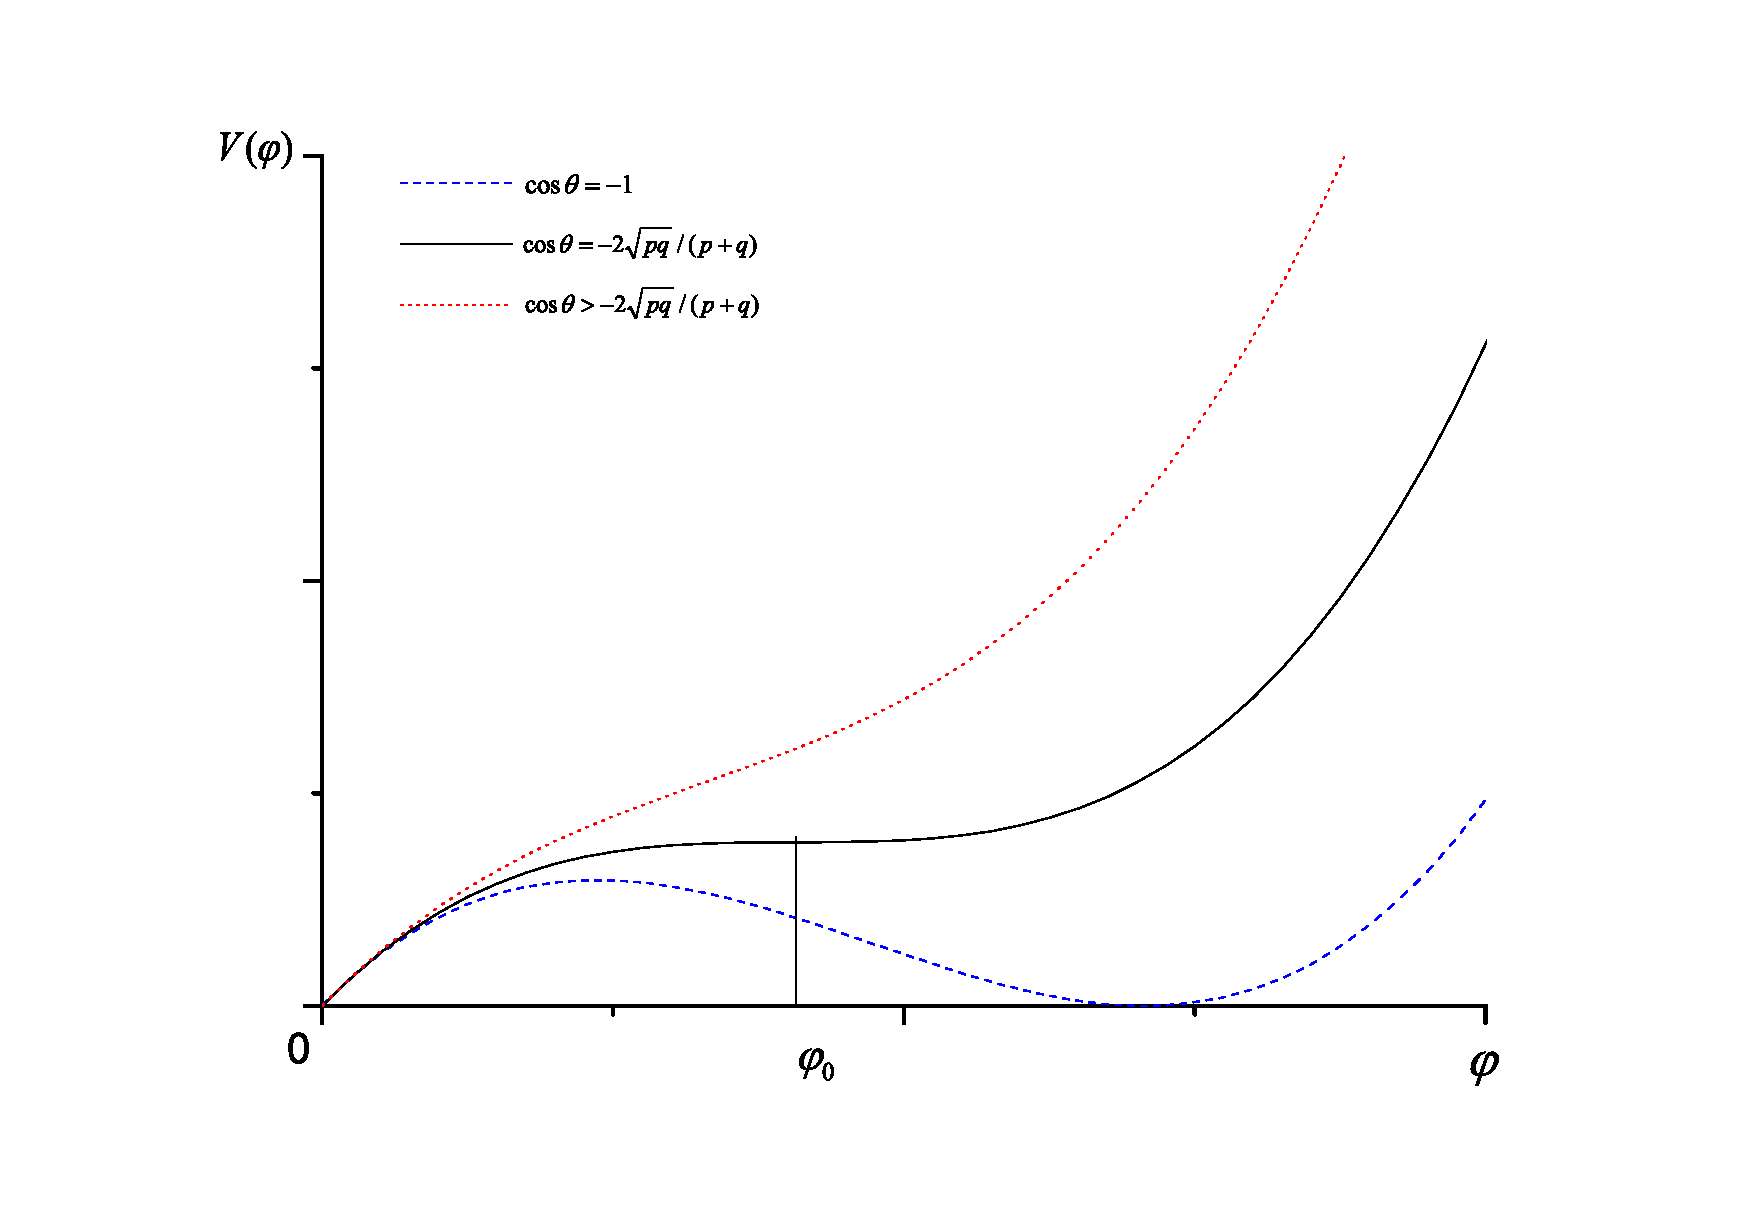
\includegraphics[width=5in]{Img/Graph1.eps}
  \caption{暴胀势能$V(\varphi)$,虚线、实线、点线分别对应$\cos\theta=-1$、$\cos=-2\sqrt{pq}/(p+q)$、$\cos>-2\sqrt{pq}/(p+q)$}\label{fig:potential-for-single-inflection-point-inflation}
\end{figure*}

我们发现当$\cos\theta =
-1$时,势能存在$\varphi=\sqrt{2}{\left(\frac{p}{\xi
q}\right)}^{\frac{n}{q-p}}$和$\varphi=0$处分别存在一个极小值,如图$(\ref{fig:potential-for-single-inflection-point-inflation})$中蓝色虚线所示。当$\cos\theta$逐渐变大,$\varphi=\sqrt{2}{\left(\frac{p}{\xi
q}\right)}^{\frac{n}{/q-p}}$处的极小值逐渐上移被抬起。如果抬起的不够高,那么暴胀场仍有可能被困在假真空之中。

有趣的情况是当$\theta$满足条件
\begin{equation}
  \label{eq:inflection-point-condition}
  \cos\theta = - \frac{2\sqrt{pq}}{p+q}. 
\end{equation}
局部最大值和右侧极小值在$\varphi_0=\sqrt{2}{\left(\frac{1}{\xi}\sqrt{\frac{p}{q}}\right)}^{\frac{n}{q-p}}$处重合,假真空消失。这个点被称为反射点,此处暴胀势能为
\begin{equation}
  V(\varphi_0) = \hat{\lambda}^2_{p} \left( \frac{p}{q}+\frac{4p}{p+q}+1\right)
  {\left(\frac{p}{\xi^2 q}\right)}^{\frac{p}{q-p}},
\end{equation}
并且势能$V$的一阶、二阶导数在$\varphi_0$处都等于零。值得注意的是反射点的势能表达式中不含$n$,表明给定不同的参数$n$在反射点的势能大小都相同。在反射点的势能大小都相同。
因为$\varphi_0$附近势能非常平坦,因此模型预言的标量谱指标以及张标比都能落在Planck
2015年数据限制的$1\sigma$置信水平的区域中。

当$\cos\theta > -
\frac{2\sqrt{pq}}{p+q}$,则势能不再有平坦的区间,将重现出势能为幂函数的暴胀模型。

另外一件值得注意的事情是当选定参数为某些值的时候,势能在原点附近是一个奇函数,这将导致暴胀场在暴胀结束后产生期待之外的行为。
不过当标量场满足条件
\begin{equation}
  \varphi < \sqrt{2} {\left(\frac{\kappa}{n^2}\right)}^{\frac{n}{2n-2}}.
\end{equation}
时,式$(\ref{eq:lagrangian-with-running-kinetic-term})$中动能项里的$\kappa$将不能忽略。正如前面小节中提到的那样,此时正则归一的动力学变量不再是$\varphi$,而是标量场$\phi$。于是对应的势能也不再是图$(\ref{fig:potential-for-single-inflection-point-inflation})$中所示,而是${\left(\sum_m
\lambda_m \left\lvert \phi \right\rvert^{m}\right)}^2$。
当$\phi$增加时,SUSY破缺质量项$m_{\phi}\left\lvert \phi\right\rvert
^2$将会主导势能变化\citep{nakayama2010running},因此标量场将会在原点附近不断振荡然后重新加热宇宙。

现在开始把注意力集中在拐点暴胀势能上。因为参数$\theta$满足条件$(\ref{eq:inflection-point-condition})$,因此当参数$n$、$p$和$q$给定时,只剩下两个自由参数$\hat{\lambda}_{p}$和$\xi$。
暴胀场的势能$(\ref{eq:scalar_potential})$将变成
\begin{equation}
  \label{eq:inflection-poin-potential}
  V(\varphi) = \hat{\lambda}^2_{p}
  {\left(\frac{\varphi}{\sqrt{2}}\right)}^{\frac{2p}{n}} 
  \left[ 1-4\xi \frac{\sqrt{pq}}{p+q}
  {\left(\frac{\varphi}{\sqrt{2}}\right)}^{\frac{q-p}{n}} + \xi^2 
{\left(\frac{\varphi}{\sqrt{2}}\right)}^{\frac{2(q-p)}{n}}\right].
\end{equation}

\subsection{慢滚近似}
式$(\ref{eq:PSRA_epsilon})$和$(\ref{eq:PSRA_eta})$为势能慢滚参数$\epsilon$和$\eta$的定义。在近似到一阶的情况下,标量功率谱指标$n_{s}$和张标比$r$用慢滚参数表示的表达式为
\begin{align}
  \label{eq:ns-in-slow-roll-parameter}
  & n_{s} \simeq 1 - 6\epsilon + 2\eta, \\
  \label{eq:eta-in-slow-roll-parameter}
  & r \simeq 16\epsilon.
\end{align}
暴胀期间的e-folding数可以用下面的积分式计算
\begin{equation}
  \label{eq:e-folding-number-with-potential-integral}
  N = \int_{\varphi_{f}}^{\varphi_{i}} \frac{V}{V^\prime} d\varphi, 
\end{equation}
$\varphi_{i}$和$\varphi_{f}$分别为暴胀开始和结束的时刻,并且$\varphi_{f}$的值由
$\text{Max} \{\epsilon(\varphi_{f}), \eta(\varphi_{f})\}=1$决定。

参数$\hat{\lambda}_{p}$的限制条件为曲率扰动的振幅
\begin{equation}
  \label{eq:amplitude-of-curvature-perturbation-by-Planck}
  \mathcal{P}_{\mathcal{R}} = \frac{V}{24\pi^2\epsilon}.
\end{equation}
根据 Planck 2015 的数据,$\mathcal{P}_{\mathcal{R}}(k_0)=2.19\times
10^{-9}$。因此给定$n,p,q$的值之后,就能得到$\hat{\lambda}_{p}$和$\xi$的关系。
针对不同的$n$、$p$、$q$的取值,我们计算了$\hat{\lambda}_{p}$和$\xi$的关系并绘制了图$(\ref{fig:Ln-1-2})$、$(\ref{fig:L2-p-4})$和$(\ref{fig:L2-1-q})$。
图$(\ref{fig:LN-50})$针对给定的$n$、$p$、$q$,但是不同的e-folding数$N=60$和$N=50$。

\begin{figure}
  \centering
  \includegraphics[width=5in]{Img/Ln,1,2.eps}
  \caption{e-folding数$N=60$,参数$(p,q)$为$(1,
  2)$,$n=2,3,4$时,为了与Planck数据给出的曲率扰动相一致,参数$\hat{\lambda}$和$\xi$必须满足的关系。}\label{fig:Ln-1-2}
\end{figure}

\begin{figure*}\small
  \centering
  \includegraphics[width=5in]{Img/L2,p,4.eps}
  \caption{e-folding数$N=60$,参数$(n,q)$为$(2,
  4)$,$p=1,2,3$时,为了与Planck数据给出的曲率扰动相一致,参数$\hat{\lambda}$和$\xi$必须满足的关系。}\label{fig:L2-p-4}
\end{figure*}

\begin{figure*}\small
  \centering
  \includegraphics[width=5in]{Img/L2,1,q.eps}
  \caption{e-folding数$N=60$,参数$(n,p)$为$(2,
  1)$,$q=2,3,4$时,为了与Planck数据给出的曲率扰动相一致,参数$\hat{\lambda}$和$\xi$必须满足的关系。}\label{fig:L2-1-q}
\end{figure*}

\begin{figure*}\small
  \centering
  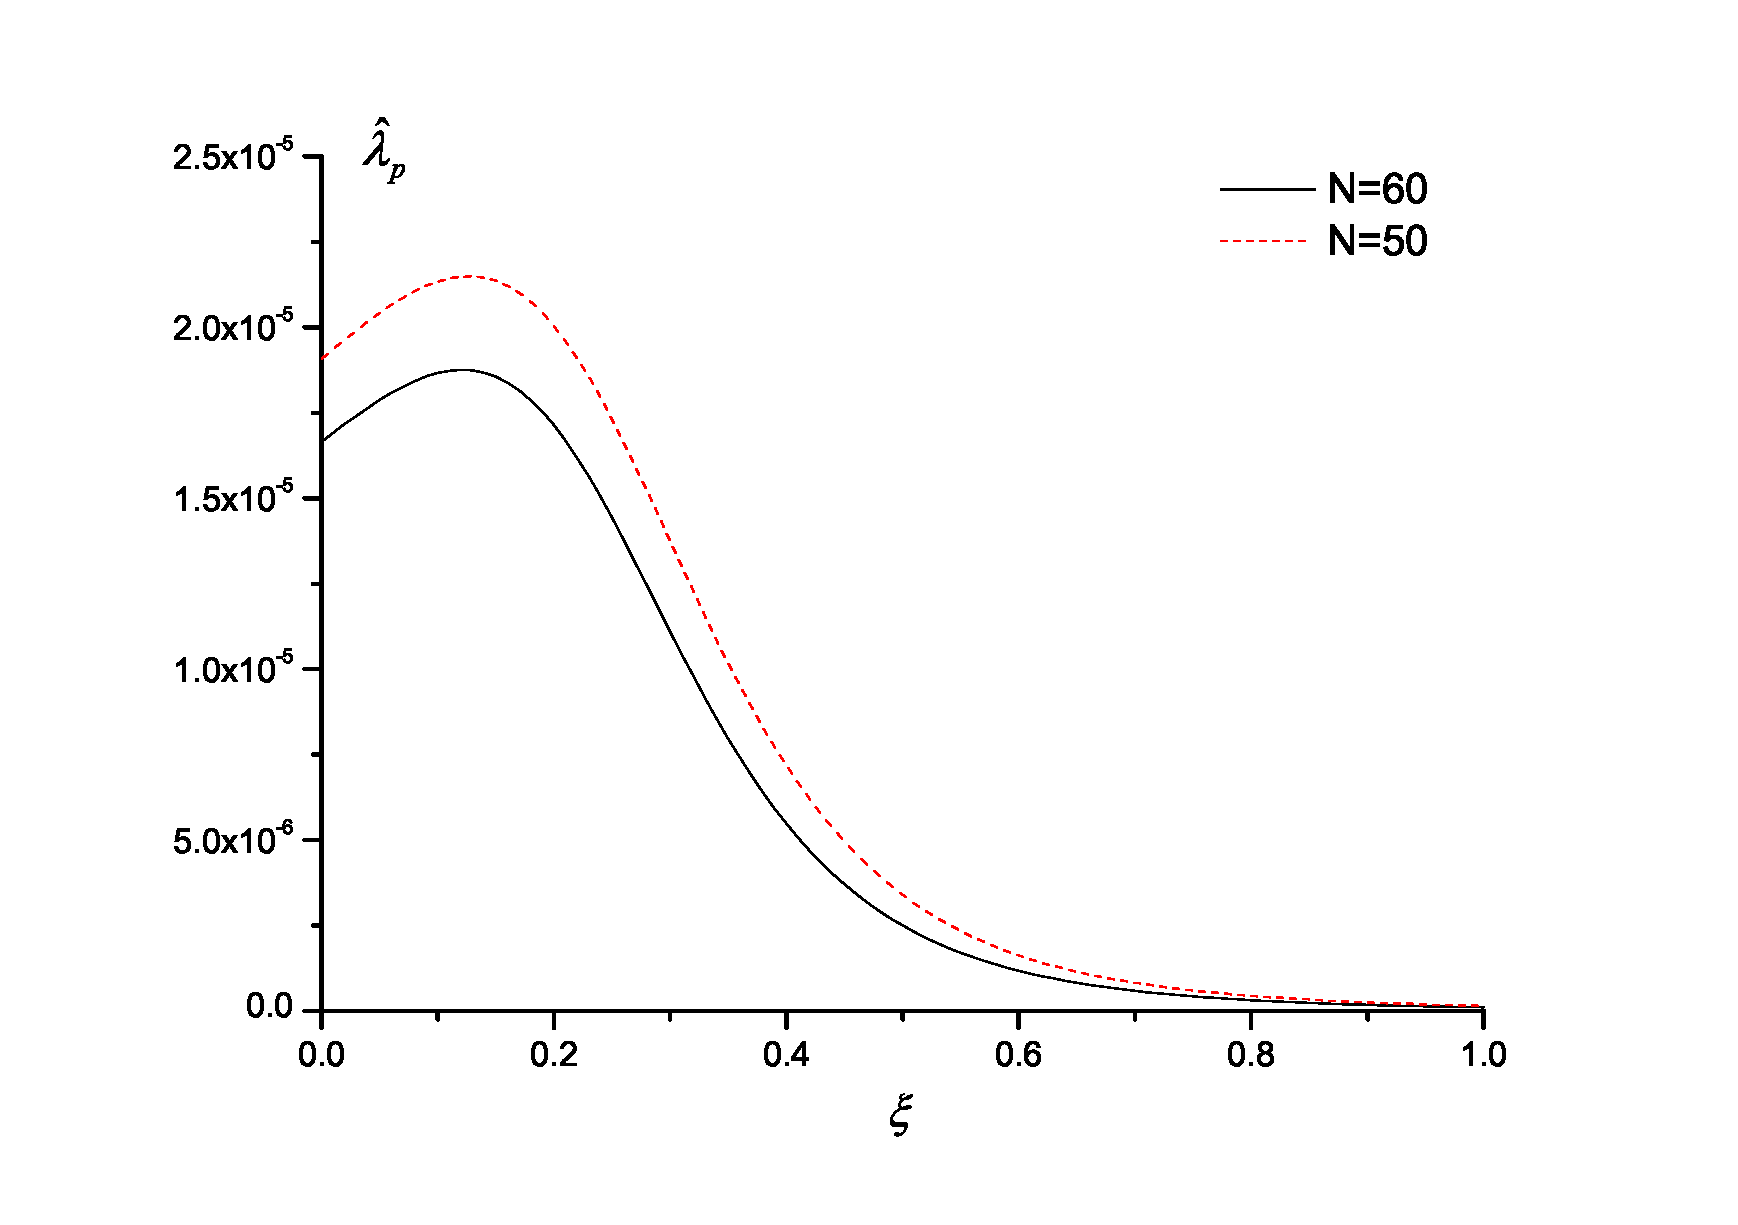
\includegraphics[width=5in]{Img/LN=50.eps}
  \caption{参数$(n,p,q)$为$(2,1,2)$,e-folding数分别为$N=60$和$N=50$时,为了与Plack数据给出的曲率扰动相一致,参数$\hat{\lambda}$和$\xi$必须满足的关系。}\label{fig:LN-50}
\end{figure*}

\begin{figure*}\small
  \centering
  \includegraphics[width=5in]{Img/Gn,1,2.eps}
  \caption{曲线是当e-folding数为$N=60$时,模型给出的$n_{s}-r$关系。等高线分别为$68\%$和$95\%$置信水平上,$n_{s}$和$r$坐落的区域,由Planck
  2015年TT+lowP数据给出,基准尺度为$k_{\star}=0.002\text{Mpc}^{-1}$。其中参数$(p,
q)$为$(1,2)$,幂指数$n$从上到下分别为$1,2,3,4$。曲线上黑点处对应参数$\xi=0$。}\label{fig:Gn-1-2}
\end{figure*}


\begin{figure*}\small
  \centering
  \includegraphics[width=5in]{Img/G2,p,4.eps}
  \caption{曲线是当e-folding数为$N=60$时,模型给出的$n_{s}-r$关系。其中参数$(n,
q)$为$(2,4)$,幂指数$p$从上到下分别为$3,2,1$。曲线上黑点处对应参数$\xi=0$。}\label{fig:G2-p-4}
\end{figure*}

\begin{figure*}\small
  \centering
  \includegraphics[width=5in]{Img/G2,1,q.eps}
  \caption{曲线是当e-folding数为$N=60$时,模型给出的$n_{s}-r$关系。其中参数$(n,
p)$为$(2,4)$,幂指数$q$从上到下分别为$4,3,2$。曲线上黑点处对应参数$\xi=0$。}\label{fig:G2-1-q}
\end{figure*}

\begin{figure*}\small
  \centering
  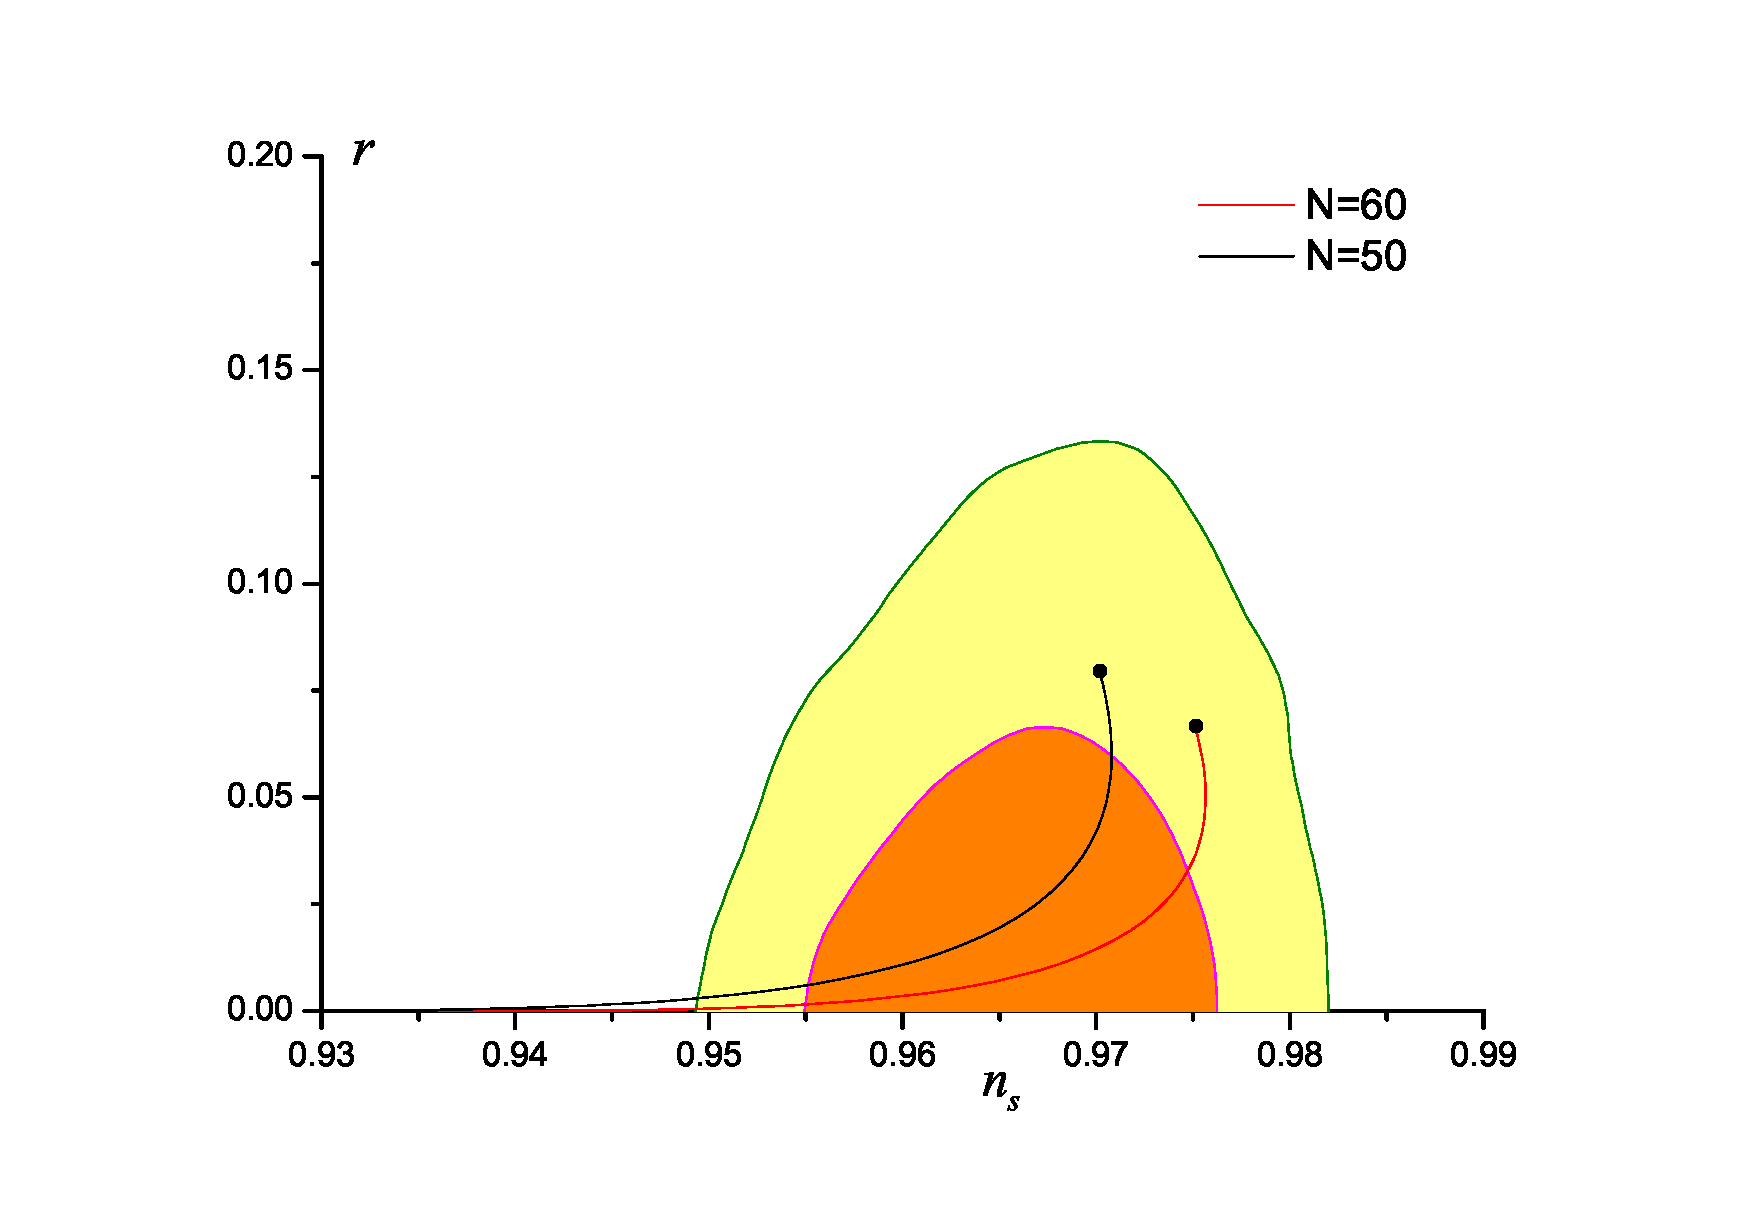
\includegraphics[width=5in]{Img/GN=50.eps}
  \caption{曲线为模型给出的$n_{s}-r$关系。其中参数$(n,
,p,q)$为$(2,1,2)$,黑色曲线和红色曲线分别对应e-folding数为$N=60$和$N=50$的数值结果。}\label{fig:GN-50}
\end{figure*}

图$(\ref{fig:Gn-1-2})$、$(\ref{fig:G2-p-4})$、$(\ref{fig:G2-1-q})$和$(\ref{fig:GN-50})$
展示了模型依据不同的$n$、$p$和$q$的值预言的$n_{s}-r$区域。等高线区域来自于
Planc 2015 年 TT+lowP
数据,基准尺度为$k_{\star}=0.002\text{Mpc}^{-1}$,$n_{s}-r$落在黄色和红色区域的可能性分别为$68\%$和$95\%$。

在图$(\ref{fig:Gn-1-2})$中,我们看到当$p=1$以及$q=2$时,随着$n$从$1$增加到$4$,曲线的位置越来越低,与
Planck
的数据越来越一致。图$(\ref{fig:G2-p-4})$中,选取参数$n=2$以及$q=4$,曲线从上到下
分别对应幂指数$p=3,2,1$。在图$(\ref{fig:G2-1-q})$中,选取参数$n=2$以及$p=1$,曲线从上到下分别对应幂指数$q=4,3,2$。可以看到三条曲线有一个汇聚点,该点正是$xi=0$的地方,也是最初势能为$V\propto
\varphi^{m
/n}$的暴胀模型给出的预言位置。图$(\ref{fig:GN-50})$中的两条曲线分别为$N=60$(黑线)和$N=50$(红线)的情况,从图中能够看出结果和
Planck 2015 的数据并不冲突。

最后,在暴胀结束后,标量场$\varphi$将会变得很小,直到$\varphi <
\sqrt{2}{\left(\kappa /n^2\right)}^{n
/(2n-2)}$后,动能项$(\ref{eq:kinetic-coefficient-of-Phi})$中的$\kappa$变得更加重要,于是标量场$\phi$取代$\varphi$成为动力学变量。这一阶段势能的形式变为${\left(\sum_m
\lambda_m \left\lvert
\phi\right\rvert^{m}\right)}^2$。随着场$\phi$继续减小,超对称破缺的质量项
$m_{\phi}\left\lvert\phi\right\rvert^2$开始主导势能的变化。
最终暴胀场将在原点附近来回振荡,通过与希格斯粒子耦合逐渐衰变为标准粒子来重新加热宇宙。这一重加热的过程和\citep{nakayama2010running}中描述的过程非常相似。


\chapter{双拐点暴胀模型预言的引力波}

前面的章节中我们讨论了在超引力中构造拐点暴胀模型。接下来我们将继续在超引力中构造暴胀模型——双拐点暴胀模型,并将其与原初黑洞相结合。

\section{超引力}

仍然考虑带有平移对称性的K\"ahler势\citep{ketov2016susy}
\begin{align}
    K=ic(\Phi-\bar\Phi)-\frac{1}{2}{(\Phi-\bar\Phi)}^2-\frac{\zeta}{4}{(\Phi-\bar\Phi)}^4,
\end{align}
其中$c$和$\zeta$为实参数。暴胀场取为手征超场$\Phi=(\phi+i\chi)/\sqrt{2}$的实部分量$\phi$。只要四次方项$\frac{\zeta}{4}{(\Phi-\bar\Phi)}^4$中的$\zeta$取得足够大,则暴胀场$\phi$在暴胀期间,场$\chi$的期望为$\langle\chi\rangle\approx0$。

参考了racetrack模型\citep{krasnikov1987supersymmetry,escoda2003saltatory,blanco2005racetrack}和其他模型\citep{ketov2016susy},我们选取如下形式的超势
\begin{align}
    W=a_0(1+a_1e^{-b_1\Phi}+a_2e^{-b_2\Phi}+a_3e^{-b_3\Phi}).
\end{align}

如果我们在宇宙学常数为零的真空中恢复来真空的超对称性(关于真空中的超对称破缺问题的讨论请参考文献\citep{gao2015inflection}),则F-term和势能V在$\Phi=0$处应当都为零,即$D_{\Phi}W=0$,$V=0$,这要求超势W满足约束条件
\begin{align}\label{eq:sp_constrain}
    W=\partial_{\Phi}W=0.
\end{align}
求解约束条件 (\ref{eq:sp_constrain}) 可以消去参数$a_1$和$a_2$
\begin{align}
    a_1\rightarrow \frac{b_2+a_3b_2-a_3b_3}{b_1-b_2},\qquad 
    a_2\rightarrow \frac{-b_1-a_3b_1+a_3b_3}{b_1-b_2}.
\end{align}
将K\"ahler势和超势代入到公式
\begin{align}
    V=e^{K/M^2_P}\lbrack
    D_{\Phi_i}W{(K^{-1})}^{ij^{\star}}D_{\Phi^{\star}_j}W^{\star}-3M^{-2}_P|W|^2\rbrack,
\end{align}
中,可以得到标量势能$V(\phi)$。其中,
\begin{align}
    D_{\Phi}W=\partial_{\Phi}W+M^{-2}_P{(\partial_{\Phi}K)}W,
\end{align}
以及K\"ahler度规的逆,
\begin{align}
    K^{ij\star} = \frac{\partial^2K}{\partial\Phi_i\partial\Phi^{\star}_j}.
\end{align}

当在参数空间中选取某组参数如
\begin{align}\label{eq:parameters}
    a_0 = 4.35\times 10^{-6},
    a_3 = 7\times 10^{-8},
    b_1 = 3.05,
    b_2 = 6.3868164,
    b_3 = -4.4,
    c = 2.8.
\end{align}
时,标量势能$V(\phi)$有两个近反射点,如图\ref{fig:potential}中所示。场取较大值处的拐点给出与当前CMB数据相一致的标量谱指标和张标比,较小值处的拐点可以使标量扰动的功率谱产生一个尖峰从而生成原初黑洞。
\begin{figure}[!htbp]
    \centering
    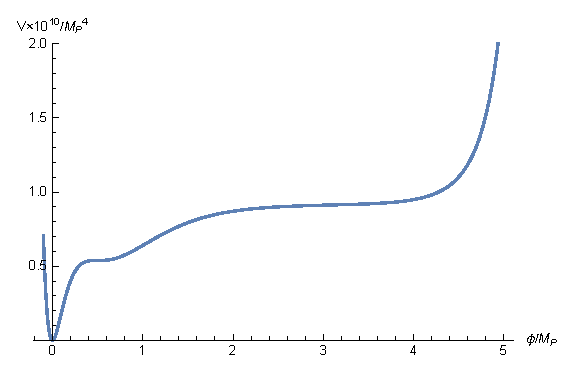
\includegraphics{Img/potential.eps}
    \caption{双拐点标量势能$V(\phi)$}\label{fig:potential}
\end{figure}

在FRW背景以及单场慢滚框架下,基于势能的慢滚参数$\epsilon_V$和$\eta_V$为
\begin{align}
    \epsilon_V &= \frac{M^2_P}{2}{\left(\frac{V\prime}{V}\right)}^2, \\
    \eta_V &= M^2_P {\left(\frac{V^{\prime\prime}}{V}\right)}.
\end{align}

由于在拐点附近势能变得极端平坦,因此慢滚近似不再适用\citep{dimopoulos2017ultra,germani2017primordial},代之以极端慢滚暴胀。此时为了更精确地求解暴胀过程,势能慢滚参数需要替换为哈勃慢滚参数\citep{schwarz2001higher,leach2002cosmological,schwarz2004primordial},
\begin{align}
    \epsilon_H &= -\frac{\dot{H}}{H^2}, \\
    \eta_H &= -\frac{\ddot{H}}{2H\dot{H}}=\epsilon_H-\frac{1}{2}\frac{d \ln\epsilon_H}{dN_e}, \\
    \xi_H &=
    \frac{\dddot{H}}{2H^2\dot{H}}-2\eta^2_H=\epsilon_H\eta_H-\frac{d\eta_H}{dN_e},
\end{align}

点$\dot{}$表示对宇宙时间$t$的导数,$N_e(t)$表示从视界穿过$k_{\star}$到暴胀结束期间的e-folding数,通常在取值在范围$50\sim60$之间。

标量谱指标及其跑动和张标比的领头阶可以用$\epsilon_H,\eta_H,\xi_H$来表示
\begin{align}
    n_s &= 1- 4\epsilon_H+2\eta_H, \\
    \alpha &= \frac{dn_s}{d\ln k}=10\epsilon_H\eta_H-8\epsilon_H^2-2\xi_H, \\
    r &= 16\epsilon_H.
\end{align}

在参数集 (\ref{eq:parameters}),相应的数值结果为
\begin{align}
    n_s = 0.9635,\qquad \alpha=-0.00369,\qquad r=0.00276,
\end{align}

当$k_{\star}=0.05Mpc^{-1}$时,在$68\%$的置信水平上与Planck
2018给出的对CMB的限制结果相一致\citep{akrami2018planck}
\begin{align}
    n_s = 0.9640\pm 0.0043,\qquad 
    \alpha = -0.0071\pm 0.0068,\qquad
    r < 0.079.
\end{align}

由于在拐点附近用近似表达式$\mathcal{P_R}\approx\frac{1}{8\pi^2M^2_P}\frac{H^2}{\epsilon_H}$计算得到的标量扰动会低于真实值\citep{gao2018primordial}。因此必须在模空间中数值求解MS方程,
\begin{align}\label{eq:ms}
    \frac{d^2u_k}{d\eta^2}+\left(k^2-\frac{1}{z}\frac{d^2z}{d\eta^2}\right)u_k=0,
\end{align}
其中$\eta$为共形时间,$z\equiv\frac{a}{\mathcal{H}}\frac{d\phi}{d\eta}$。初值条件取为Bunch-Davies真空\citep{bunch1978quantum}
\begin{align}
    u_k\rightarrow\frac{e^{-ik\eta}}{\sqrt{2k}},\quad\text{as}\quad
    \frac{k}{aH}\rightarrow\infty.
\end{align}

出于数值求解的方便,我们将共形时间$\eta$替换为$N_e$,把MS方程重写为\citep{ballesteros2018primordial}
\begin{align}
    \frac{d^2u_k}{dN^2_e}+\left(1-\epsilon_H\right)\frac{du_k}{dN_2}+
    \lbrack\frac{k^2}{\mathcal{H}^2}+\left(1+\epsilon_H-\eta_H\right)\left(\eta_H-2\right)-\frac{d\left(\epsilon_H-\eta_H\right)}{dN_e}=0,
\end{align}
原初功率谱由下式给出
\begin{align}
    \mathcal{P_R}=\frac{k^3}{2\pi^2}\lvert\frac{u_k}{z}\rvert^2_{k\ll
    \mathcal{H}}
\end{align}

图\ref{fig:pert}为MS方程\ref{eq:ms}基于参数集\ref{eq:parameters}的数值结果。从图中可以发现功率谱在小尺度有一个高峰,在CMB的尺度上大约增长了7个数量级。这样大的一个密度扰动使得原初黑洞能够通过引力塌缩形成。

\begin{figure}[!htbp]
    \centering
    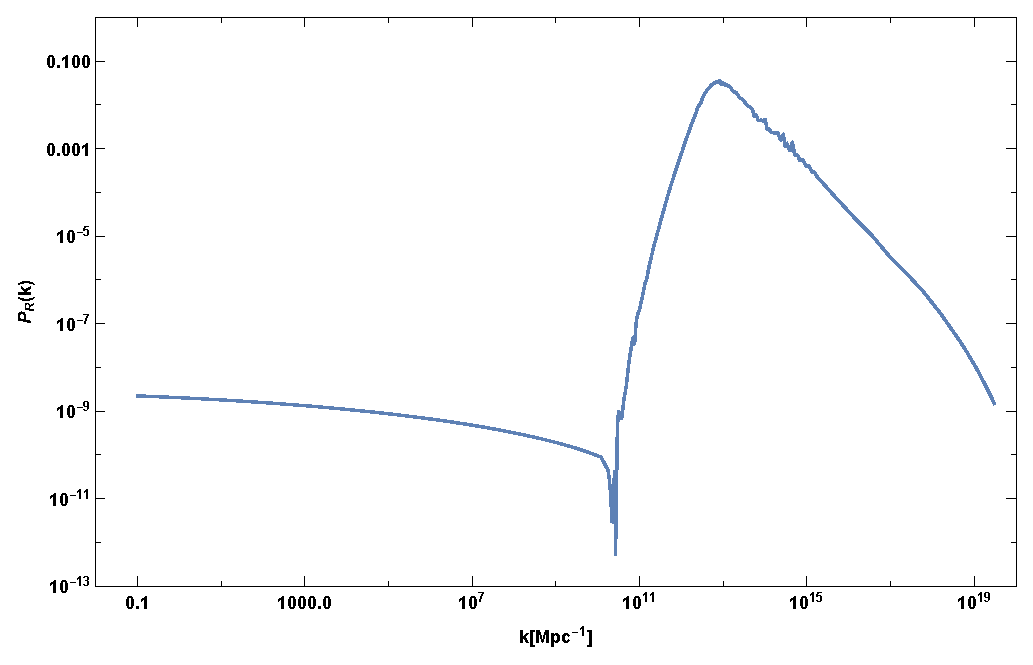
\includegraphics[width=4in]{Img/pert.eps}
    \caption{双拐点暴胀模型预测的标量扰动的原初功率谱$\mathcal{P_R}$}\label{fig:pert}
\end{figure}

\section{在超引力中构造双拐点暴涨模型}
在第三章中曾提到在超引力中构造暴涨模型通常采用双场理论。通常我们期望暴涨过程中
演化方程只涉及暴涨场,因而要求其它的标量场稳定在使势函数取极值处。
在某些模型中,需要特别注意辅助场$S$在$s=0$处的稳定性。
有两种方法可以做到,一是在K\"ahler势中添加项$S\bar{S}$,二是选择不含标量自由度
的手征场$S$作为辅助场。后一种方法中涉及描述宇宙演化的只有一个无约束的手征超场$\Phi$场。
基于此,产生了一类无需引入额外非约束手征超场就能描述当前宇宙演化的暴涨模型
\citep{kallosh2015inflation,dall2014sgoldstino,linde2015does} 。


后来,Ketov和Terada提出了一类基于单手征超场$\Phi$的新暴涨理论
\citep{ketov2014generic,ketov2014inflation}。在 \citep{ketov2014generic}
中,提出了一种新的对数形式的K\"ahler势
\begin{equation}
  \label{eq:logarithmic-kahler-potential}
  K =
-3\ln \left[1+\frac{\Phi+\bar{\Phi}+\zeta{\left(\Phi+\bar{\Phi}\right)}^{4}}{\sqrt{3}}\right].
\end{equation}
$\zeta$是常系数。其中超场$\Phi$通常被分解为实部$\phi$和虚部$\chi$
\begin{equation}
  \Phi = \frac{1}{\sqrt{2}}(\phi+i\chi). 
\end{equation}
由于该K\"ahler势在平移变换$\Phi\rightarrow
\Phi+iC$下是不变的,超场$\Phi$的虚部$\chi$不会出现在K\"ahler势中,因此可以作为
暴涨场的候选者。在这个K\"ahler势中,四次方项的作用是在暴涨过程中将场$\phi$
稳定在零附近。并且K\"ahler势中并没有加入平方项和三次方项,尽管这些项不破坏对称
性,但是相应的系数可以通过调节超场$\Phi$和其它超场之间的耦合而压低。

不论超势取何种形式,当K\"ahler势取$(\ref{eq:logarithmic-kahler-potential})$式时,场$\Phi$的动能项系数为
\begin{equation}
  \label{eq:kinetic-coefficient-of-Phi}
  G(\phi,\chi) =
  \frac{3(1+32\zeta^2\phi^{6}-8\zeta\phi^2(3\sqrt{3}+\sqrt{2}\phi))}{{\left(\sqrt{3}+\sqrt{2}\phi+4\zeta\phi^{4}\right)}^2}.
\end{equation}

\begin{figure}[!http]
  \centering
  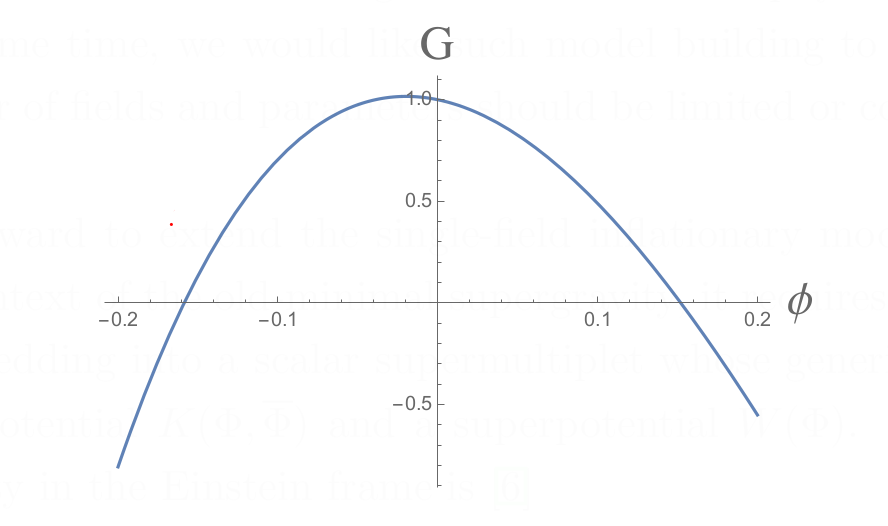
\includegraphics[width=5in]{Img/kinetic_coefficient_for_Phi.png}
  \caption{$\zeta=1$时,手征场$\Phi$的动能项系数与$\phi$的函数关系}\label{fig:kinetic-coefficient_for_Phi}
\end{figure}

从图$(\ref{fig:kinetic-coefficient_for_Phi})$可知,为了使$G>0$,$\phi$被限制在一
个有限的区间内。$\zeta$越大,$\phi$的取值区间越窄。因而在暴涨期间,标量场$\phi$的影响可以忽略,暴涨势近似为暴涨场$\chi$的函数,K\"ahler势中四次方项的调节作用
在这里清晰地体现出来了。当超势为
\begin{equation}
  W = \frac{1}{\sqrt{2}} f(-\sqrt{2}i\Phi),
\end{equation}
其中,$f$为实函数,沿暴涨场方向的暴涨势为
\begin{equation}
  V\simeq {\left[f_{,\chi}(\chi)\right]}^2.
\end{equation}
暴涨结束后,场朝着全局最小值滚去,最终得到一个超对称闵可夫斯基真空。这种情况对一
大类的超势都成立,同时也期望能在此基础上通过对K\"ahler势作一个微小的修正,能够抬升真空能得到德$\cdot$西特真空。然而no-go定理\citep{kallosh2014analytic}告诉我们对K\"ahler势和超势作一个无穷小修改,无法将具有超对称的闵可夫斯基真空连续地变化到德$\cdot$西特真空。举一个例子,当超势取如下形式时
\begin{equation}
  W=m(c\Phi+1),  
\end{equation}
\begin{figure}
  \centering
  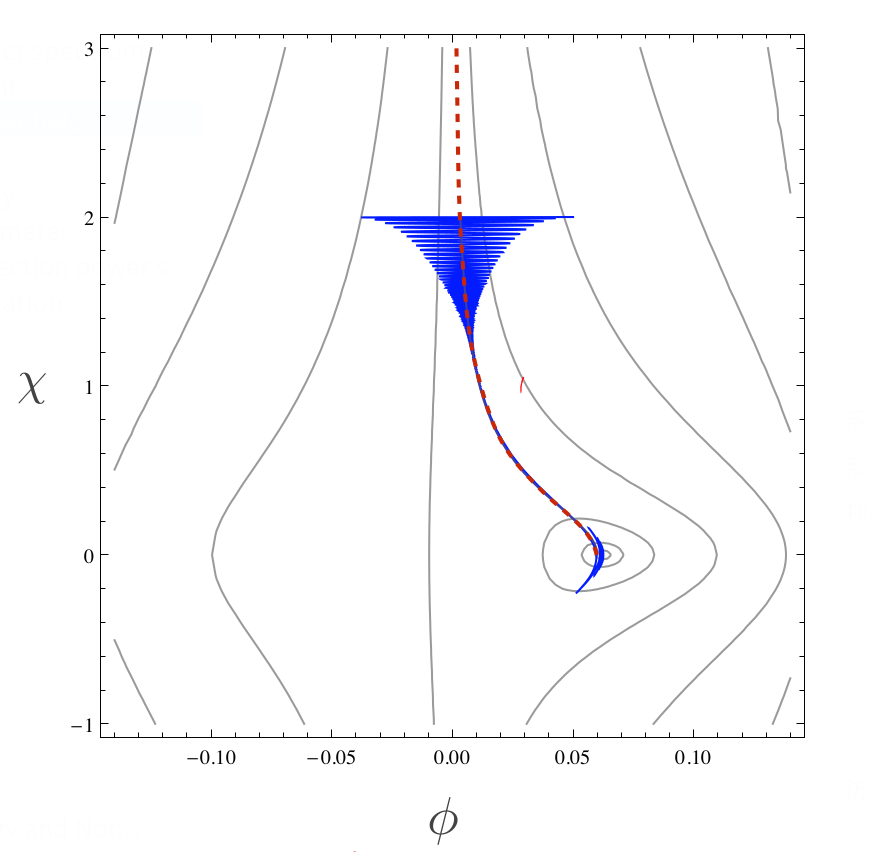
\includegraphics[width=5in]{Img/potential-for-linear-superpotential.png}
  \caption{蓝实线为数值计算得到的暴涨场的演化过程,红虚线为有效暴涨势的绝热近似。黑实线为暴涨势$V(\phi(\chi),
  \chi)$的对数等高线。当暴涨场靠近吸引子解前以及暴涨结束后都有一个震荡阶段。}\label{fig:potential-for-linear-superpotential}
\end{figure}
$c$和$d$为实参数,在$\phi=0$方向上暴涨势为
\begin{equation}
  V(\phi=0,\ \chi)=m^2c(c-2\sqrt{3}).
\end{equation}
显然参数$c$的大小将决定暴涨势大于零还是小于零。更具体的分析会发现,暴涨发生的过程并不完全在$\phi=0$方向。从图$(\ref{fig:potential-for-linear-superpotential})$中可以
看到,暴涨结束后得到的是一个超对称破缺的闵可夫斯基真空。通过对参数$c$进行微小的调节就能得到预期的德$\cdot$西特宇宙,$V_0\sim
10^{-120}$。但是代价为引起了强超对称破缺,得到的引力微子质量$m_{3/2}$比通常
理论预期的TeV量级高出多个量级。当考虑到粒子物理标准模型的时候,暴涨结束后是否
恢复超对称性是一件很重要的事情。例如
\citep{endo2006moduli,nakamura2006gravitino,kawasaki2006gravitino,kawasaki2006gravitino-overproduction,asaka2006gravitinos}
指出当真空超对称性破缺时,早期宇宙中从暴涨场衰变得到的引力微子数目会增多,
而这将引起灾难。另外\citep{degrassi2012higgs}中指出如果超对称破缺的能标过高,
电弱真空会遇到稳定性问题。

为了规避上述困难,同时在不破坏no-go定理的前提下,有两种方法既能抬升真空势能
得到德$\cdot$西特真空又能避免大的超对称破缺。一是引入额外的手征多态
(Polonyi场),并且对其施加强约束尽可能降低其对宇宙演化的影响
\citep{dudas2013strong}。另一个方法是引入零幂手征超场
\citep{ferrara2014cosmology,kallosh2015inflation,dall2014sgoldstino,kallosh2015inflation-de-sitter,linde2015does},
并且能从弦论中找到理论解释\citep{kallosh2014emergence}。

沿着这个思路,\citep{ketov2016susy}讨论了暴涨结束后恢复超对称性的条件,以及通过添加一个满足零幂条件$S^2=0$的Polonyi超场作为超对称破缺场$S$来控制超对称破缺的能标。


仍然考虑带有平移对称性的K\"ahler势\citep{ketov2016susy}
\begin{align}
    K=ic(\Phi-\bar\Phi)-\frac{1}{2}{(\Phi-\bar\Phi)}^2-\frac{\zeta}{4}{(\Phi-\bar\Phi)}^4,
\end{align}
其中$c$和$\zeta$为实参数。暴涨场取为手征超场$\Phi=(\phi+i\chi)/\sqrt{2}$的实部分量$\phi$。只要四次方项$\frac{\zeta}{4}{(\Phi-\bar\Phi)}^4$中的$\zeta$取得足够大,则暴涨场$\phi$在暴涨期间,场$\chi$的期望为$\langle\chi\rangle\approx0$。

参考了racetrack模型\citep{krasnikov1987supersymmetry,escoda2003saltatory,blanco2005racetrack}和其他模型\citep{ketov2016susy},我们选取如下形式的超势
\begin{align}
    W=a_0(1+a_1e^{-b_1\Phi}+a_2e^{-b_2\Phi}+a_3e^{-b_3\Phi}).
\end{align}

如果我们在宇宙学常数为零的真空中恢复了真空的超对称性
(关于真空中的超对称破缺问题的讨论请参考文献
\citep{gao2015inflection}),则F-term和暴涨势V在$\Phi=0$处应当都为零,
即$D_{\Phi}W=0$,$V=0$,这要求超势W满足约束条件
\begin{align}\label{eq:sp_constrain}
    W=\partial_{\Phi}W=0.
\end{align}
求解约束条件 (\ref{eq:sp_constrain}) 可以消去参数$a_1$和$a_2$
\begin{align}
    a_1\rightarrow \frac{b_2+a_3b_2-a_3b_3}{b_1-b_2},\qquad 
    a_2\rightarrow \frac{-b_1-a_3b_1+a_3b_3}{b_1-b_2}.
\end{align}
将K\"ahler势和超势代入到公式
\begin{align}
    V=e^{K}\lbrack
    D_{\Phi_i}W{(K^{-1})}^{ij^{*}}D_{\Phi^{*}_j}W^{*} - 3|W|^2\rbrack,
\end{align}
中,可以得到标量势$V(\phi)$。其中,
\begin{align}
    D_{\Phi}W=\partial_{\Phi}W + {(\partial_{\Phi}K)}W.
\end{align}
以及K\"ahler度规的逆,
\begin{align}
    K^{ij*} = \frac{\partial^2K}{\partial\Phi_i\partial\Phi^{*}_j}.
\end{align}

当在参数空间中选取某组参数如
\begin{align}\label{eq:parameters}
    a_0 = 4.35\times 10^{-6},
    a_3 = 7\times 10^{-8},
    b_1 = 3.05,
    b_2 = 6.3868164,
    b_3 = -4.4,
    c = 2.8.
\end{align}
时,标量势$V(\phi)$有两个近反射点,如图\ref{fig:potential}中所示。
场取较大值处的拐点给出与当前CMB数据相一致的标量功率谱的谱指标和张标比,
较小值处的拐点可以使标量扰动的功率谱产生一个尖峰从而生成原初黑洞。
\begin{figure}[!htbp]
    \centering
    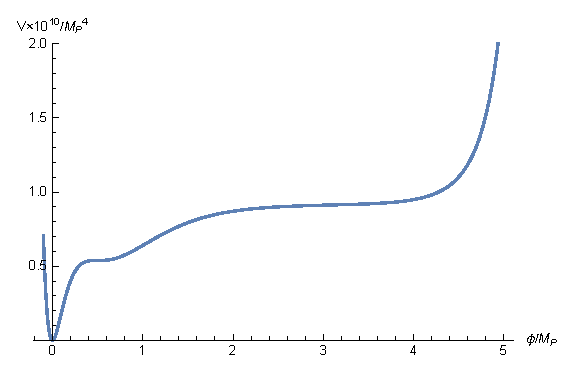
\includegraphics[width=5in]{Img/potential.eps}
    \caption{双拐点标量势$V(\phi)$}\label{fig:potential}
\end{figure}

在FLRW背景以及单场慢滚框架下,基于势能的慢滚参数$\epsilon_V$和$\eta_V$为
\begin{align}
  \epsilon_V &= \frac{1}{2}{\left(\frac{V_{,\phi}}{V(\phi)}\right)}^2, \\
  \eta_V &= \frac{V_{,\phi \phi}}{V(\phi)}.
\end{align}

由于在拐点附近暴涨势变得极端平坦,因此慢滚近似不再适用\citep{dimopoulos2017ultra,germani2017primordial},代之以极端慢滚暴涨。此时为了更精确地求解暴涨过程,势能慢滚参数需要替换为哈勃慢滚参数\citep{schwarz2001higher,leach2002cosmological,schwarz2004primordial},
\begin{align}
    \epsilon_H &= -\frac{\dot{H}}{H^2}, \\
    \eta_H &= -\frac{\ddot{H}}{2H\dot{H}}=\epsilon_H-\frac{1}{2}\frac{d \ln\epsilon_H}{dN_e}, \\
    \xi_H &=
    \frac{\dddot{H}}{2H^2\dot{H}}-2\eta^2_H=\epsilon_H\eta_H-\frac{d\eta_H}{dN_e},
\end{align}
其中,$N_e(t)$表示从视界穿过$k_{\star}$到暴涨结束期间的e-folding数,通常在取值在范围$50\sim60$之间。

标量扰动谱指标及其跑动和张标比的领头阶可以用$\epsilon_H,\eta_H,\xi_H$来表示
\begin{align}
    n_s &= 1- 4\epsilon_H+2\eta_H, \\
    \alpha &= \frac{dn_s}{d\ln k}=10\epsilon_H\eta_H-8\epsilon_H^2-2\xi_H, \\
    r &= 16\epsilon_H.
\end{align}

在参数集 (\ref{eq:parameters})下,相应的数值结果为
\begin{align}
  n_s &= 0.9635,\\
  \alpha&=-0.00369,\\
  r&=0.00276,
\end{align}

当$k_{\star}=0.05Mpc^{-1}$时,在$68\%$的置信水平上与Planck
2018给出的对CMB的限制结果相一致\citep{akrami2018planck}
\begin{align}
  n_s &= 0.9640\pm 0.0043,\\
  \alpha &= -0.0071\pm 0.0068,\\
  r &< 0.079.
\end{align}

标量扰动的功率谱在慢滚暴涨模型通常用近似公式
\begin{equation}
  \label{eq:scalar-perturbation-power-spectrum}
  \mathcal{P}_{\mathcal{R}} = \frac{V}{24\pi^2 \epsilon_V}.
\end{equation}
计算得到。由于在拐点处,暴涨势导数为零,因此使用势能慢滚参数的功率谱近似公式在
拐点处产生无穷大,导致公式失效。因而
\citep{germani2017primordial,motohashi2017primordial}中采用了不同的近似公式,
由于哈勃慢滚参数在整个暴涨期间始终大于零,因此基于哈勃慢滚参数的近似功率谱公式
\begin{equation}
  \label{eq:scalar-perturbation-power-spectrum-hubble}
  \mathcal{P}_{\mathcal{R}} \simeq
  \frac{1}{8\pi^2}\frac{H^2}{\epsilon_H}.
\end{equation}
将会给出更准确的结果。不过仍然指出这种近似可能会导致对PBH的质量函数产生错误的
估计,因而 \citep{ballesteros2018primordial}中根据Mukhanov-Sasaki (MS)公式
\citep{sasaki1986large,mukhanov1988quantum}数值求解精确的功率谱。 
Mukhanov-Sasaki (MS)方程为
\begin{align}\label{eq:ms}
    \frac{d^2u_k}{d\eta^2}+\left(k^2-\frac{1}{z}\frac{d^2z}{d\eta^2}\right)u_k=0,
\end{align}
其中$\eta$为共形时间,$z\equiv\frac{a}{\mathcal{H}}\frac{d\phi}{d\eta}$。初值条件取为Bunch-Davies真空\citep{bunch1978quantum}
\begin{align}
    u_k\rightarrow\frac{e^{-ik\eta}}{\sqrt{2k}},\quad\text{as}\quad
    \frac{k}{aH}\rightarrow\infty.
\end{align}

出于数值求解的方便,我们将共形时间$\eta$替换为$N_e$,把MS方程重写为\citep{ballesteros2018primordial}
\begin{align}
    \frac{d^2u_k}{dN^2_e}+\left(1-\epsilon_H\right)\frac{du_k}{dN_2}+
    \lbrack\frac{k^2}{\mathcal{H}^2}+\left(1+\epsilon_H-\eta_H\right)\left(\eta_H-2\right)-\frac{d\left(\epsilon_H-\eta_H\right)}{dN_e}=0,
\end{align}
原初功率谱由下式给出
\begin{align}
    \mathcal{P_R}=\frac{k^3}{2\pi^2}\left\lvert\frac{u_k}{z}\right\rvert^2_{k\ll
    \mathcal{H}}.
\end{align}

图\ref{fig:pert}为MS方程\ref{eq:ms}基于参数集\ref{eq:parameters}的数值结果。从图中可以发现功率谱在小尺度有一个高峰,在CMB的尺度上大约增长了7个数量级。这样大的一个密度扰动使得原初黑洞能够通过引力塌缩形成。

\begin{figure}[!htbp]
    \centering
    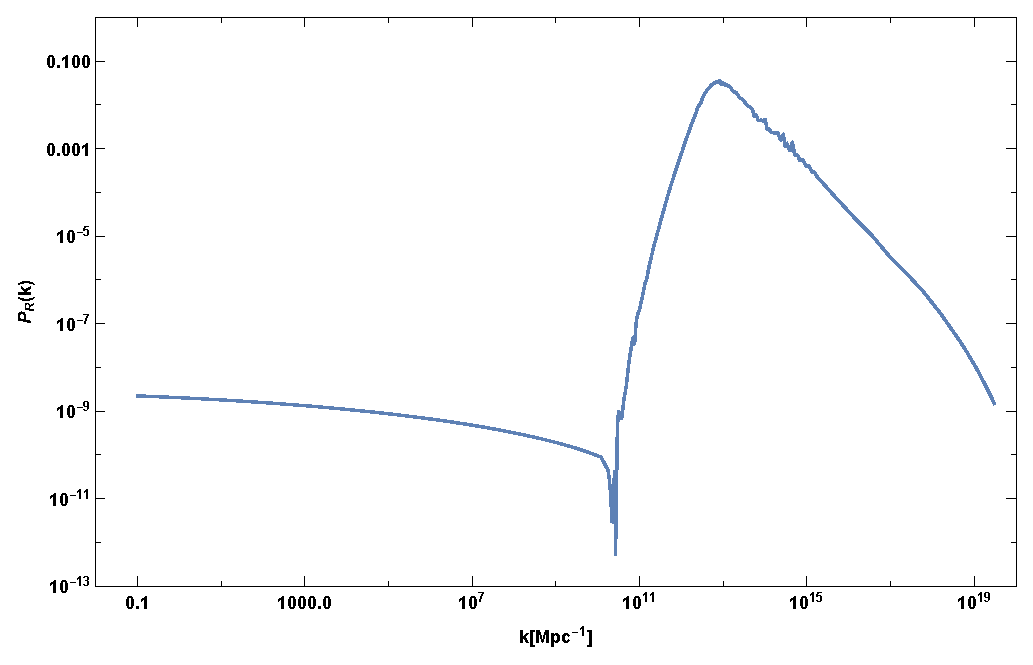
\includegraphics[width=5in]{Img/pert.eps}
    \caption{双拐点暴涨模型预测的标量扰动的原初功率谱$\mathcal{P_R}$}\label{fig:pert}
\end{figure}

\section{原初黑洞}
当某个原初密度扰动足够大的尺度在暴涨结束后重新进入视界时,由引力塌缩可能形成原初黑洞。
一般黑洞的质量$M$正比于当时的一个哈勃体积内的总质量$M_H$,比例系数为$\gamma$。
\begin{equation}
    M = \gamma M_H = \gamma \frac{4}{3}\pi\rho H^{-3}
\end{equation}
系数$\gamma$取决于引力塌缩的过程,与采取的模型有关,一般取
$0.2$在辐射为主时期\citep{carr1975primordial}。利用熵守恒$d(g_s(T)T^3a^3)/dt=0$和$\rho\propto
g(T)T^4$,可以得到辐射为主时期:
\begin{equation}
    \label{eq:mass_pbh}
    M=\gamma M_{H(eq)}{\left(\frac{g(T_f)}{g(T_{eq})}\right)}^{1/2}
    {\left(\frac{g_s(T_f)}{g_s(T_{eq})}\right)}^{-2/3}
    {\left(\frac{k}{k_{eq}}\right)}^{-2}
\end{equation}

$M_{H(eq)}$表示辐射-物质相等时的视界内的总质量。因为物质为主时期
$H^2\propto \rho \propto a^{-3}$和 $k=aH$,故有
\begin{align*}
    \label{eq:horizon_mass_eq}
    M_{H(eq)} &= \frac{4}{3}\pi\rho_{eq}H_{eq}^{-3} \\
    &= \frac{4}{3}\pi\rho_m
    a_{eq}^{-3}{\left(\frac{k_{eq}}{a_{eq}}\right)}^{-3}\\
    &= \frac{4}{3}\pi \Omega_m \rho_{0,crit}k^{-3}_{eq} \\
    &\approx 3\times 10^{50}\ g
\end{align*}

在辐射为主时期假设 $g(T)=g_s(T)$
是一个好的近似,以及最新Planck
2018数据\citep{aghanim2018planck}给出的$k_{eq}=0.073\Omega_m
h^2\ \text{Mpc}^{-1}$。于是{(\ref{eq:mass_pbh})}可写成
\begin{equation}
    M(k) =
    10^{18}g\left(\frac{\gamma}{0.2}\right){\left(\frac{g(T_f)}{106.75}\right)}^{-1/6}
    {\left(\frac{k}{7\times10^{13}\ \text{Mpc}^{-1}}\right)}^{-2}
\end{equation}
$M(k)$表示共动波数$k$重新进入视界时形成的黑洞的质量。

在Press-schechter引力塌缩模型中\citep{press1974formation},质量M的原初黑洞的生成率由一个高斯随机概率分布决定。当相对密度扰动$\delta$大于某个阈值$\delta_c$时,视界内的物质将在引力的作用下塌缩形成一个黑洞,那么质量为M的原初黑洞所占丰度$\beta(M)$将由高斯分布的分布函数给出:
\begin{align}
    \label{eq:mass_fraction_pbh}
    \beta(M) = \frac{1}{\sqrt{2\pi \sigma^2(M)}}\int_{\delta_c}^{\infty}
    d\delta\ \text{exp}\left(\frac{-\delta^2}{2\sigma^2(M)}\right).
\end{align}

唯一不确定的还剩下方差$\sigma^2(M)$。对它的计算一般采用如下方式,将空间粗粒化成一个个尺度为$R=1/k$的区域,并用高斯窗口函数$W(x)=\text{exp}(-x^2/2)$将相对密度扰动光滑化,最后对所有区域求$\delta$的方差作为$\sigma^2(M)$:
\begin{align}
    \sigma^2(M(k)) &= \int \frac{dq}{q}W{(qR)}^2 \\
    &= \frac{16}{81}\int \frac{dq}{q} {(qR)}^4 \mathcal{P_R}(q)W{(qR)}^2,
\end{align}

对应$k$模的原初黑洞对暗物质的贡献为
\begin{align*}
    f_{PBH}(M) &\equiv \frac{\Omega_{PBH}(M)}{\Omega_c} =
    \frac{\rho_{PBH}(M)}{\rho_m}\mid_{eq}\frac{\Omega_m h^2}{\Omega_c h^2}
    \\
    &= \frac{\beta(M)}{8\times
    10^{-16}}{\left(\frac{\gamma}{0.2}\right)}^{3/2}{\left(\frac{g(T_M)}{106.75}\right)}^{-1/4}{\left(\frac{M}{10^{18}\ g}\right)}^{-1/2}
\end{align*}

其中暗物质的丰度取为$\Omega_c h^2 \simeq 0.12$\citep{aghanim2018planck}。当前所有原初黑洞的丰度由积分式给出;
\begin{align}
    \label{eq:abundence_pbh}
    \Omega_{PBH} = \int \frac{dM}{M}\Omega_{PBH}(M),
\end{align}

公式{(\ref{eq:mass_fraction_pbh})}说明原初黑洞的质量分数对临界塌缩密度$\delta_c$非常敏感。在辐射为主时期,近期多数在这方面的研究文章\citep{musco2005computations,musco2009primordial,musco2013primordial,harada2013threshold}建议$\delta_c$取值大约为$0.45$。此时若希望原初黑洞能在$\mathcal{O}(1)$量级成为暗物质组成成分,那么曲率扰动的原初功率谱需要增大到大约为$\mathcal{P_R}\simeq
10^{-2}$。而在CMB尺度上,扰动大约为$\mathcal{P_R}\simeq
10^{-9}$。因此我们需要一个机制,使得对应某个尺度范围(相应的某个原初黑洞的质量区间)的曲率扰动在离开视界时产生一个峰。

把原初黑洞的质量和e-folding数联系起来,能使我们对其形成于哪个时期有一个相对清晰的概念。为了做到这一点,需要假设在暴涨时期,哈勃“常数”近似为常数。所以$k$模离开视界时相对于某个基准$k_\star$已经膨胀了大约
\begin{align}
    \label{eq:delta_efolding}
    \Delta N^{\star}_e = \log \frac{a_k}{a_\star} = \log\frac{a_k
    H_I}{k_\star} = \log \frac{a_f H_f}{k_\star},
\end{align}
仍然假设对应熵和能量密度的有效自由度数相等,于是可以得到公式\citep{motohashi2017primordial}:
\begin{align}
    \Delta N^{\star}_e =
    -\frac{1}{2}\log\frac{M}{M_\odot}+\frac{1}{2}\log\gamma
    +\frac{1}{12}\log\frac{g(T)}{106.75}+\frac{1}{2}\log\frac{4.4\times10^{24}\Omega_r
    H^2_0}{k^2_{\star}}, 
\end{align}
其中辐射密度为$\Omega_r h^2=4.18\times10^{-5}$,哈勃常数为$H_0\simeq
0.0007\text{Mpc}^{-1}$。若选择基准为$k_\star =
  0.05\text{Mpc}^{-1}$,参考Planck组的数据,上式可以变为
\begin{align}
    \Delta N^{\star}_e = 18.37-\frac{1}{2}\log\frac{M}{M_\odot}.
\end{align}



\section{引力波}


\chapter{总结与展望}%
\label{chap:summary}
本文


%---------------------------------------------------------------------------%
% main content
%-
%-> Appendix
%-
\cleardoublepage%
\appendix% initialize the environment
\chapter{中国科学院大学学位论文撰写要求}

学位论文是研究生科研工作成果的集中体现,是评判学位申请者学术水平、授予其学位的主要依据,是科研领域重要的文献资料。根据《科学技术报告、学位论文和学术论文的编写格式》(GB/T 7713-1987)、《学位论文编写规则》(GB/T 7713.1-2006)和《文后参考文献著录规则》(GB7714—87)等国家有关标准,结合中国科学院大学(以下简称“国科大”)的实际情况,特制订本规定。

\section{论文无附录者无需附录部分}

\section{测试公式编号} \label{sec:testmath}

\begin{equation} \label{eq:appedns}
    \adddotsbeforeeqnnum%
    \begin{cases}
        \frac{\partial \rho}{\partial t} + \nabla\cdot(\rho\Vector{V}) = 0\\
        \frac{\partial (\rho\Vector{V})}{\partial t} + \nabla\cdot(\rho\Vector{V}\Vector{V}) = \nabla\cdot\Tensor{\sigma}\\
        \frac{\partial (\rho E)}{\partial t} + \nabla\cdot(\rho E\Vector{V}) = \nabla\cdot(k\nabla T) + \nabla\cdot(\Tensor{\sigma}\cdot\Vector{V})
    \end{cases}
\end{equation}
\begin{equation}
    \adddotsbeforeeqnnum%
    \frac{\partial }{\partial t}\int\limits_{\Omega} u \, \mathrm{d}\Omega + \int\limits_{S} \unitVector{n}\cdot(u\Vector{V}) \, \mathrm{d}S = \dot{\phi}
\end{equation}
% appendix content
%-
%-> Backmatter: bibliography, glossary, index
%-
\backmatter% initialize the environment
\intotoc*{\cleardoublepage}{\bibname}% add link to toc
\bibliography{Biblio/ref}% bibliography
\chapter{作者简历及攻读学位期间发表的学术论文与研究成果}

\textbf{本科生无需此部分}。

\section*{作者简历}

\subsection*{casthesis作者}

吴凌云,福建省屏南县人,中国科学院数学与系统科学研究院博士研究生。

\subsection*{ucasthesis作者}

莫晃锐,湖南省湘潭县人,中国科学院力学研究所硕士研究生。

\section*{已发表(或正式接受)的学术论文:}

[1] ucasthesis: A LaTeX Thesis Template for the University of Chinese Academy of Sciences, 2014.

\section*{申请或已获得的专利:}

(无专利时此项不必列出)

\section*{参加的研究项目及获奖情况:}

可以随意添加新的条目或是结构。

\chapter[致谢]{致\quad 谢}\chaptermark{致\quad 谢}% syntax: \chapter[目录]{标题}\chaptermark{页眉}
\thispagestyle{noheaderstyle}% 如果需要移除当前页的页眉
%\pagestyle{noheaderstyle}% 如果需要移除整章的页眉

感激casthesis作者吴凌云学长,gbt7714-bibtex-style
开发者zepinglee,和ctex众多开发者们。若没有他们的辛勤付出和非凡工作,\LaTeX{}菜鸟的我是无法完成此国科大学位论文\LaTeX{}模板ucasthesis的。在\LaTeX{}中的一点一滴的成长源于开源社区的众多优秀资料和教程,在此对所有\LaTeX{}社区的贡献者表示感谢!

ucasthesis国科大学位论文\LaTeX{}模板的最终成型离不开以霍明虹老师和丁云云老师为代表的国科大学位办公室老师们制定的官方指导文件和众多ucasthesis用户的热心测试和耐心反馈,在此对他们的认真付出表示感谢。特别对国科大的赵永明同学的众多有效反馈意见和建议表示感谢,对国科大本科部的陆晴老师和本科部学位办的丁云云老师的细致审核和建议表示感谢。谢谢大家的共同努力和支持,让ucasthesis为国科大学子使用\LaTeX{}撰写学位论文提供便利和高效这一目标成为可能。

\cleardoublepage[plain]% 让文档总是结束于偶数页,可根据需要设定页眉页脚样式,如 [noheaderstyle]

% other information
\end{document}
%---------------------------------------------------------------------------%

